% =========================================================================
% Copyright (c) 2008-2014 Audio Communication Group, TU Berlin
% 
% This file is part of WhisPER, a package of interacting MATLAB scripts for 
% designing and controlling experiments in the field of auditory perceptive 
% measurement and evaluation.
% 
% WhisPER is free software: you can redistribute it and/or modify it under 
% the terms of the GNU General Public License as published by the Free 
% Software Foundation, either version 3 of the License, or (at your option) 
% any later version. 
% 
% WhisPER is distributed in the hope that it will be useful, but WITHOUT ANY 
% WARRANTY; without even the implied warranty of MERCHANTABILITY or FITNESS 
% FOR A PARTICULAR PURPOSE.
% See the GNU General Public License for more details.
%
% You should have received a copy of the GNU General Public License along 
% with this program. If not, see <http://www.gnu.org/licenses/>. 
%
% Version of WhisPER: 1.9.0
% 
% http://www.ak.tu-berlin.de/whisper/ 
% =========================================================================%
% 
% This file:
%
% Author 	:   	Simon Ciba, student at FG Audiokommunikation, TU Berlin
% Email  	:   	sciba2 AT hotmail DOT com
% Date   	:   	17-Nov-2008
% Updated	:   	2-Dec-2014 update to WhisPER 1.9.0 
%					-FBrinkmann: added \section{ITU-R Rec. BS.1116-1 (ABC/HR) \& ITU-R Rec. BS.1534-1 (MUSHRA)}
% 
%					17-Apr-2014 update to WhisPER 1.8.1
%					- changed in saqi_items_english.m: 
%					- from "reverberation level" to "level of reverberation"
%					- from "reverberation time" to "duration of reverberation"
%					
%					03-Feb-2014 update to WhisPER 1.8.0, changed version numbering to X.Y.Z 
%                   - (X = major changes, Y= new tests, Z = bugfixes), added SAQI (EN/GER), 
%                   - updated infos on ABX (data export, randomization), typos, 
%					- added articles: 	lindau:2014a %SAQI-EN
%										lindau:2014b %SAQI-GER
%										lindau:2015 %SAQI-Manual
%								
%					10-Jan-2011 XML/GRD file formats; Johannes Blickensdorff (hannes at blickensdorff dot com)
%					- updated: export section \section{Basic concept}\label{concept} in whisper-userdoc.tex
%  				    - Article{fromm:2004} in literature.bib
% 					- introduced: \paragraph{Other File Formats: GridXML and GRD}		 
%					
%					05-Jun-2009 14:00 license changed
% 					10-May-2009 13:45 update of few general information (new url of project website, etc.)
% 					19-Nov-2008 13:25 comments on the rgt's configuration
%            		
% =========================================================================
%
%                           whisper-userdoc.tex
% 
% =========================================================================
%
%
%-------------------------------------------
% preamble
%-------------------------------------------

\documentclass[a4paper,11pt, twoside, liststotoc, bibtotoc, halfparskip-, pointlessnumbers, normalheadings, openany]{scrreprt} % using Koma-Script

% character encoding
\usepackage[latin1]{inputenc}
\usepackage[english]{babel}
% single quotation marks
\newcommand{\lqq}{``}
\newcommand{\rqq}{''}
\renewcommand{\lq}{`}
\renewcommand{\rq}{'}
\usepackage{marvosym}
\usepackage{acronym}
% citation 
%\usepackage[sort,authoryear]{natbib}
\usepackage[sort]{natbib}
% captions
\usepackage[format=hang,
						font={footnotesize, sf},
						labelfont={bf},
						margin=1cm,
						aboveskip=5pt,
						position=bottom]{caption}
% page layout			
\usepackage{vmargin}
\setmarginsrb{3.0cm}{1.5cm}{2.5cm}{1.5cm}{7mm}{1.2cm}{4mm}{1.5cm}
% font
\usepackage[scaled]{helvet}
% embedding graphics
\usepackage[pdftex]{graphicx}
% landscape format
\usepackage{lscape}
% captions beyond sliding figures
\usepackage{capt-of} 
% include pdfs
\usepackage{pdfpages}
% composite figures
\usepackage{subfig}
% persistent pagination
\usepackage{remreset}
% special symbols -> (R)
\usepackage{amssymb} 
\makeatletter
\@removefromreset{footnote}{chapter}
\makeatother
% including external file content (needed for the ltxtables)
\usepackage{filecontents}
% specific definitions for this document
\newcommand{\whisper}{{\sc WhisPER}}
\newcommand{\whisperversion}{1.9.0} 
\newcommand{\dateofdocumentversion}{Feb. 5th, 2015} 
% designing head and foot lines
\usepackage{fancyhdr}
% multirow table 
\usepackage{multirow}
\usepackage{longtable}

% redefinition of page style 'plain'
\fancypagestyle{plain}{
\fancyhead{}%lschen der Vorbelegung
\fancyhead[LO]{\nouppercase{\textit\rightmark}}
\fancyhead[RE]{\nouppercase{\textit\leftmark}}
\fancyhead[RO, LE]{\sffamily\bfseries\thepage}
\fancyfoot[C]{\footnotesize\whisper\ v\whisperversion\ -- User Documentation}
}
% definition of the document's standard page style
\fancypagestyle{standard}{
\fancyhead{}%lschen der Vorbelegung
\fancyhead[LO]{\nouppercase{\textit\rightmark}}
\fancyhead[RE]{\nouppercase{\textit\leftmark}}
\fancyhead[RO, LE]{\sffamily\bfseries\thepage}
\fancyfoot[C]{\footnotesize\whisper\ v\whisperversion\ -- User Documentation}
}
% activation of the standard page style
\pagestyle{standard}
% redefinition of chapter and section marks
\renewcommand{\chaptermark}[1]{%
\protect\markboth{\thechapter.~ #1}{}%
}
\renewcommand{\sectionmark}[1]{%
\protect\markright{\thesection~ #1}%
}
% bottom of the page ragged (needed because of Koma-Script's 'twoside' option)
\raggedbottom
% re-formatting of the minisection superscription
\setkomafont{minisec}{\bigskip\rmfamily}

% redefinition of the description environment (kill the vertical space)
\makeatletter 
\renewenvironment{description}
               {\list{}{\labelwidth\z@ \itemindent-\leftmargin
                        \let\makelabel\descriptionlabel} \setlength{\itemsep}{0ex} \setlength{\parskip}{0mm} \setlength{\topsep}{0mm} \setlength{\partopsep}{0mm}}
               {\endlist}
\makeatother           
% depth of section numbering
\setcounter{secnumdepth}{3}
\setcounter{tocdepth}{3}
% fixed column width in tables
\usepackage{tabularx}
% setting formulas
\usepackage{empheq}
% hyperlinks, urls and document properties
\usepackage[pdftitle = {WhisPER - user documentation}, pdfauthor = {Simon Ciba}]{hyperref}\urlstyle{rm} 



%-------------------------------------------
% properly document
%-------------------------------------------


\begin{document}


% titlepage
\begin{titlepage}\centering
\vspace*{5cm}
\Huge \bfseries{\whisper\ \LARGE v\whisperversion}\\
\vspace*{1cm}
\LARGE User Documentation\\
\vfill
\large Authors: Simon Ciba, Fabian Brinkmann, and Alexander Lindau.\\
\end{titlepage}
\clearpage
% information on author, the program and the document version; liability exclusion
\vspace*{\fill}

This document was originally created by Simon Ciba while being a student at the Audio Communication Group, TU Berlin, and completed in its first issue in November 17th, 2008. It is part of the software package \whisper\ which has been developed by Andr� Wlodarski and Simon Ciba within the scope of their master's theses conducted at TU Berlin. 

Currently, this document is maintained by Fabian Brinkmann and Alexander Lindau (Audio Communication Group, TU Berlin).

Additions to both this document and the software package \whisper\ have been contributed by both Fabian Brinkmann, and Alexander Lindau, as well as by master students Matthias Herder, Andreas Rotter, Johannes Blickensdorff, and Martina Vrhovnik.

\textit{Note:} The authors does not assume any liability for the correctness of this document's content and further takes no responsibility for any harm or damage resulting from its application.\vspace{1cm}

Date of document version: \dateofdocumentversion.


%table of contents
\tableofcontents

%list of abbreviations
\cleardoublepage\chapter*{List of Abbreviations}
\addcontentsline{toc}{section}{List of abbreviations}
\thispagestyle{plain}
\markboth{List of abbreviations}{List of abbreviations}

\vspace{1cm}
\begin{acronym}[TDMA]
	\acro{AP}{adaptive psychophysical procedure}
	%\acro{ASIO}{audio stream input/output}
	\acro{DW}{dialog window (used in a generalized meaning, cp. annot.~\ref{dw} on p.~\pageref{dw})}
	%\acro{GPL}{GNU General Public License}
	\acro{GUI}{graphical user interface}
	\acro{ID}{identification}
	\acro{LAN}{local area network}
	\acro{ML}{maximum likelihood}
	\acro{OSC}{open sound control}
	\acro{PEST}{parameter estimation by sequential testing}
  \acro{QUEST}{quick estimation by sequential testing}
	\acro{RGT}{repertory grid technique}
	\acro{SD}{semantic differential}
	\acro{ZEST}{zippy estimation by sequential testing}
	\acro{SAQI}{Spatial Audio Quality Inventory}
\end{acronym}
\vspace*{\fill}
\pagebreak



%-----------------------------------------
% CHAPTER 1
%-----------------------------------------
\cleardoublepage
\chapter{Introduction}
\section{What is \whisper ?}
\whisper\ is a package of scripts running under MATLAB\circledR\ for performing listening tests in the field of auditory perceptual research, thereby, \whisper\ is designed for maximum usability. Hence, most of the handling can be done by usage of a coherent graphical user interface (GUI) system. The aim of \whisper\ is to provide experimenters in the auditory field with a selection of the most popular listening test procedures while allowing for a convenient automation with respect to user interactions and stimulus playback. For an overview of the currently implemented listening test procedures see sec.~\ref{sec:testprocedures}.

\section{History, Versions and Availability}\label{history}
\whisper\ was developed by Andr� Wlodarski and Simon Ciba within the scope of their master's theses (\cite{ciba:2008}, \cite{wlodarski:2008}) at the Audio Communication Group of the TU Berlin, in 2008. Today, \whisper\ is continuously developed by the staff of the Audio Communication group. So far, updates included feature upgrades and the extension by multiple new test methods. Information about the history of software updates and the latest version can be read from the file \textit{release\_notes.txt} (see sec.~\ref{toplevel}). 
\\
\\
Since its version 1.8.0 \whisper\ is freely distributed using the electronic data repository DepositOnce of the Technische Universit�t Berlin. DepositOnce allows persistent identification of the current \whisper\ version using the DOI (Digital Object Identifier) \url{http://dx.doi.org/10.14279/depositonce-31}. A more informative project website can be reached from \url{http://www.ak.tu-berlin.de/whisper}.

\section{Folders and Files}\label{folders}
The current version of \whisper\ maybe freely dowloaded from DepositOnce (see ~\ref{history}) as a self-contained zip-file. After unpacking you will find four folders and some informative text files on top level. In the following, the folder and file structure will be shortly explained.

\subsection{The top-level folder \lq whisper\_X.Y.Z \rq}\label{toplevel}
The name of the top level folder contains the current \whisper\ version number. Small changes in \whisper\ (such as, e.g., bugfixes) are reflected by a changes of the rightmost version number ("Z"). Larger updates, such as, e.g., the implementation of new listening test procedures are reflected in a incrementation of the midmost version number ("Y"). The leftmost number ("X") has not changed since \whisper 's first release and is reserved for indicating in-depth changes of the whole software.

The top level folder of the \whisper\ distribution hosts the file \textit{release\_notes.txt} which contains information on the history of updates and the current software version. The file \textit{license\_notes.txt} contains the license information, while \textit{Copying.txt} contains a copy of the GNU General Public License. The file \textit{authors.txt} contains the names of all those, who contributed to \whisper\ so far. 

\subsection{The folder \lq 1 literature\rq}\label{lit}
This sub folder contains some publications giving background information on the implemented procedures or on the development of \whisper itself.

\subsection{The folder \lq 2 mfiles\rq}\label{mfiles}
This sub folder contains the main \whisper\ installation in the form of a number of MATLAB\circledR\ scripts, figures, and data files. In order to execute \whisper\ you will have to add this folder to MATLAB\circledR's path and run 'whisper' from the MATLAB\circledR\ prompt (see ~\ref{running}).

\subsection{The folder \lq 3 doc\rq}\label{doc}
This sub folder includes the user documentation, i.e. the document you are currently reading, and a technical documentation, intended to be helpful when aiming at extending \whisper's functionalities. If you plan to extend \whisper -- which is of course greatly appreciated -- it might be a good idea to get in contact with the Audio Communication Group before.

\section{License Terms}
For license information consult the file \textit{license\_notes.txt} (see sec.~\ref{doc}) which is to be found in the top level folder of the \whisper\ installation.

\section{Warranty and Safety Information}
\emph{The use of the program --~or any of its components (including this document)~-- for whatever purpose, is under the complete and
sole responsibility of the user. The authors of \whisper\ do not extend any kind of warranty.}  
\\
Special attention is drawn to the fact that \whisper\ does \emph{not} comprise an automatic mechanism to prevent the delivery of too high sound pressure levels.  It is the explicit responsibility of the user to make sure that the stimuli in use, in combination with any further playback equipment (sound card, amplifier, headphone or loudspeaker, etc.), will yield a sound pressure level, that will not cause any damage to anyones health, especially the hearing system.





%-----------------------------------------
% CHAPTER 2
%-----------------------------------------

\chapter{A Short Characterization of the Program's Features}


\section{Basic Concepts}\label{concept}
In empirical auditory research experimenters often want to administer a number of different listening tests to a number of ever identical subjects while the individual tests differ only slightly in specification (\textit{factorial within-subjects test design}). Hence, in order to simplify the administration of such tests the user interface system of \whisper\ is designed to allow a central control of multiple test procedures from one point of the system. For this purpose the program provides the administration of all data -- including the empirical test results -- from within a virtual environment called \textit{test series}, which is structurally represented by one conjoint data folder (see sec.~\ref{testseries}). 

Moreover, \whisper\ allows performing several successive -- and even interleaved -- sub-tests within one test run while applying different test procedures. This feature tries to meet some specific requirements of experimental research. For example, it is often desired to carry out a familiarization experiment immediately before starting the actual listening test. Likewise, in adaptive threshold estimation procedures, researcher often want to interleave adaptation runs for different test conditions in order conceal the actual stimulus variation this way aiming at a suppression of anticipation effects in test subjects.

Empirical data export to applications for statistical analysis such as, e.g., SPSS or MS-Excel is feasible via automatically generated formatted results text files (*.csv format). Moreover, data from repertory grid experiments (see sect. \ref{sec:testprocedures}) may be imported into specialized software packages such as Idiogrid (\url{http://www.idiogrid.com/}) and Gridsuite (\url{http://www.gridsuite.de/}) through support of their respective native results data formats GridXML and GRD (see sec.~\ref{subfolder_export}).

\section{Implemented Test Procedures}\label{sec:testprocedures}
In the present state, \whisper\ provides about seven different listening test procedures. In the following, these procedures and their basic features will be briefly reviewed together with some essential literature. More detailed information on the first three procedures (AP, RGT, and SD) can be found in the master theses of Simon Ciba (\cite{ciba:2008}), and Stefanie Otto (\cite{otto:2008}), see also ~\ref{lit}.

\begin{description}
\item[Adaptive Psychophysical Threshold Procedures:] A group of test procedures that aim at achieving efficient estimates of a single point on a psychometric function that is called a psychophysical threshold. This is achieved by adapting the intensity of the stimulus according to the history of preceding responses of the subject. There are different \textit{adaption mechanisms} and \textit{method for estimating the final threshold} from the observed response pattern. \whisper\ currently supports \textit{simple} and \textit{transformed staircase} procedures with the adaption rules 1-down/1-up, 2-down/1-up and 3-down/1-up, halving of step sizes after a predefined number of reversals and a calculation of the threshold estimate by averaging stimulus intensities over a defined number of last reversals. 
\\
\\
Furthermore, more sophisticated adaptation methods can be chosen from, such as e.g. \textit{parameter estimation by sequential testing (PEST)}, and a modified version of PEST referred to as \textit{More Virulent PEST}. Moreover, maximum likelihood and Bayesian adaption methods, such as, e.g. the \textit{Best PEST} have been implemented. Finally, \textit{QUEST} and \textit{ZEST} procedures have been implemented, too.
\\
\\
\textit{References:}
\begin{itemize}
\item Overview: \cite{treutwein:1995}, \cite[][pp.~159]{gescheider}, \cite{leek:2001} 
\item Staircase: \cite{cornsweet:1962}, \cite{wetherill:1963}, \cite{levitt:1971}, 
\item PEST: \cite{taylor:1967}
\item More Virulent PEST: \cite{findlay:1978}
\item ML/Bayesian procedure: \cite{pentland:1980}, \cite{lieberman:1982}, \cite{treutwein:1995}, \cite{treutwein:1997}
\item QUEST:\cite{watson:1983}
\item ZEST: \cite{king:1994}
\end{itemize}
\medskip
At present, \whisper\ allows employing these adaption procedures in detection and discrimination tasks while using \textit{n-alternative forced choice (nAFC)} response paradigms for n=2, 3 or 4 alternatives. Furthermore, arbitrary adaptation tracks using the same response paradigm may be randomly interleaved.
\medskip
\item[Repertory Grid Technique (RGT):] RGT is a combination of auditory attribute elicitation and scaling used for the sensory evaluation of complex stimuli. During the first part of the procedure, stimuli (called \textit{elements}) are combined to groups of three (called \textit{triads}) and presented to the subject which is supposed to report on similarities and contrasts in a qualitative manner. The result of each triad comparison is a pair of verbal expressions that are likely to represent the end-point descriptors of a bipolar attribute referred to as a \textit{construct}. In the second part of the procedure all elements are rated on bipolar scales which were formed by using the elicited constructs. 
\\
The formation of triads can be carried out manually by the experimenter or automatically by the program by creating a complete variation. Furthermore, the order of presentation of triads and elements can be defined either by the user or be generated randomly. Elicited constructs may be edited by the experimenter in between the two parts of the procedure.
\\
\\
\textit{References:} \cite[54]{bech:2006}, \cite{berg:1999}, \cite[187]{bortz_doering}, \cite{fransella:1977}, \cite{kelly:1955}  
\medskip
\item[Semantic Differential (SD):] The Semantic Differential is a procedure for rating (direct scaling) the perceived amount of a certain auditory quality while being exposed to a specific sound stimulus. Arbitrary sets of bipolar rating scales maybe defined for forming a Semantic Differential. In \whisper, the experimenter may define the presentation order of objects or he might choose a randomly generated sequence.
\\
\\
\textit{References:} \cite{osgood:1967},\cite[][pp.~185]{bortz_doering}, 
\medskip
\item[ABX-Test:] The ABX-test (also: duo-trio test) is a method for assessing the detectability of subtle differences between two stimuli. In audio technology research ABX-testing gained some publicity when being used for the controlled assessment of differences between (valve and transistor type) amplifiers or similar devices/technologies which are typically expected to exhibit only very small perceptual differences. 
\\
During an ABX-test, two stimuli A and B are to be directly compared to a third stimulus X which is deliberately chosen to be either A or B. The subject's task is to identify whether X equals stimulus A or B. The required number of trials (repetitions) reflecting a certain type-1 error level, effect size and test power may be calculated based on the binomial distribution. In \whisper the procedure is implemented as a double blind test in order to prevent investigator effects.
\\
\\ 
\textit{References:} \cite{clark:1991}, \cite{leventhal:1986}, \cite{burstein:1988}
\medskip
\item[Spatial Audio Quality Inventory:] The Spatial Audio Quality Inventory is a collection of qualitative descriptors which may be used for a differentiated, comparative auditory assessment of real, imagined and simulated acoustic environments in order to reveal specific shortcomings of a simulation under test and allow for a directed technical improvement. The SAQI comprises 48 verbal descriptors of perceptual qualities assumed to be of practical relevance in the scope of virtual acoustic environments. The SAQI is implemented as a widely customizable questionnaire-type listening test mostly operationalizating its items with continuous or categorical rating scales or multiple choice check boxes. Additionally, since \whisper\ vs. 1.9.0 the SAQI is available as a multiple-stimulus test, too. Hence, multiple stimuli may be assessed while referring to one SAQI item utilizing panels with multiple ratings scales. SAQI is further available in a German and an English version, a French version is currently under development. 
\\
\\
\textit{References:} \cite{lindau:2014a}, \cite{lindau:2014b}, \cite{lindau:2015}
\medskip %Alex
\item[ITU-R Rec. BS.1116-1 (ABC/HR) \& ITU-R Rec. BS.1534-1 (MUSHRA):] ABC/HR and MUSHRA are methods for rating multiple conditions against one or more references for instance in terms of difference (ABC/HR) or degradation (MUSHRA). ABC/HR includes for each tested condition an individual detection task according to the ABX or duo-trio paradigm (see above) and should be used when differences between test and reference conditions are expected to be small. In contrast, MUSHRA is typically recommended for the assessing intermediate sensory differences.
\\
\\
\textit{References:} \cite{ITURBS1116:1997}, \cite{ITURBS1534:2003}, \cite{bech:2006}
\end{description}

\section{System and Software Requirements}
\begin{description}
\item[Operating system] \whisper\ was developed to be executed on a 32-bit version of Windows Vista. It has also been tested on a 32-bit version of Windows XP. Usage of the software under different operating systems like Linux or OS\,X has generally been enabled although not extensively been tested.
\medskip
\item[Running environment (MATLAB\circledR\ version)] Implementation of the software package was done on MATLAB\circledR\ version 7.4.0.287 (Release 2007a), additions have been made using MATLAB\circledR\ version 7.9.0.529 (Release 2009b). Version 1.9.0 of \whisper\ was tested to run on MATLAB\circledR\ 2013a. It might be possible that earlier versions of MATLAB\circledR\ allow using \whisper, too. However, it is known that it at least a MATLAB\circledR\ from v7.0 upwards is required (not tested, though). 
\\\\
\textbf{\emph{Important note:}}
Since vs.1.8.0 the OSC (Open Sound Control) remote control  capabilities of \whisper\ are realized by using Mark Marijnssen's script \textit{\textbf{oscsend.m}} which is freely available from MATLAB\circledR\ Central and which depends on MATLAB\circledR 's Instrument Control Toolbox. 
\\\\
\textbf{This implies that - for full OSC-capabilities - \whisper\ will now require the Instrument Control Toolbox (included in  MATLAB\circledR 's student version) to be pre-installed.}

\medskip
\item[Display resolution] The GUI system requires a display resolution of at least 1280x800 pixels.
\medskip
\item[Playback environment] Presentation of the acoustical stimuli can be realized by playing .wav files from a \textit{Direct Sound}-compatible sound card \footnote{This applies to the Windows operating system. On other operating systems make sure MATLAB\circledR 's \textit{audioplayer}-object does work with your sound card.}. Another option is to send OSC messages via network protocol to some external audio player application (for instance \textit{puredata}). This way, any type OSC-compatible playback periphery can be controlled. Per stimulus event, one may send up to 6 independent OSC commands simultaneously, allowing controlling a number of different playback devices (acoustical, optical, opto-acoustical, etc.)at once \footnote{Technically speaking, MATLAB\circledR\ executes the six OSC-commands in sequence. However, normally this proceeds very quickly unless the execution is not purposely delayed by difining a number of suitable delay times.}. 
\end{description}


%-----------------------------------------
% CHAPTER 3
%-----------------------------------------

\chapter{Running the Program}\label{running}
To start \whisper, there have to be the following three steps taken in given order:
\begin{enumerate}
	\item Start MATLAB\circledR\ .
	\item Define the path of the program folder \lq 2 mfiles\rq\ as the current (working) directory in MATLAB\circledR. This can either be done by using the 		\textit{Current Directory Browser} or using the function cd (change directory) by typing \textit{cd('PathofProgramFolder')} into the command window and afterwards pressing \textit{return}.
	\item Start \whisper\ by typing \textit{whisper} into the MATLAB\circledR\ command window and afterwards pressing \textit{return}.
\end{enumerate}

After the conduction of these steps the GUI system's main window will appear which is labeled as \textit{WhisPER}. It will be described in the next section.





%-----------------------------------------
% CHAPTER 4
%-----------------------------------------

\chapter{The Main Window}
The starting point of any action is the GUI system's main window which is labeled as \whisper\ and appears right after starting the program as described in chapter~\ref{running}.  All functionality is available directly or indirectly from this part of the user interface system. Some functions can be addressed by using the \textit{menu bar}, some by using control elements placed on the main window's \textit{desktop} and some in both ways. The following two subsections supply an overview and a short description of the functionality contained in the main window.

\begin{figure}[h]\centering
	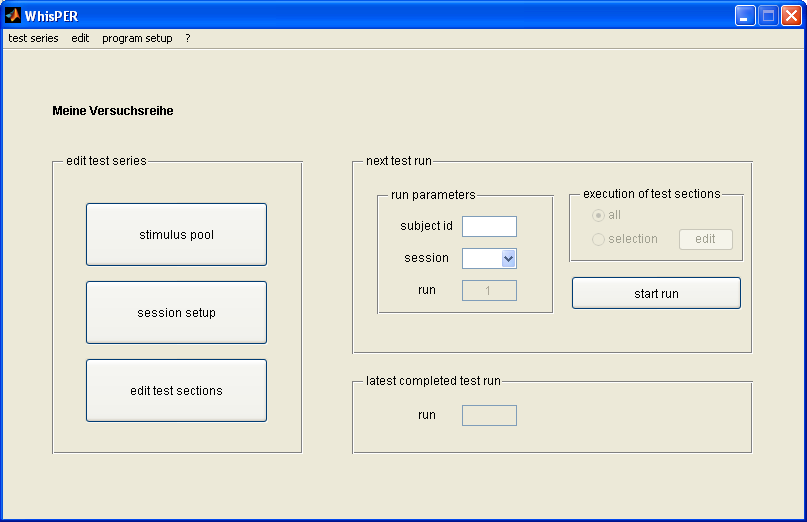
\includegraphics[resolution=150]{mainwindow.png}
  	\caption{The \textit{main window}.}
    \label{fig:mainwindow}
\end{figure}


\section{Menu Bar}\label{menubar}
This subsection describes the items in the main window's drop-down menu bar.

\minisec{Main window (menu bar)}\medskip
\begin{description}
	\item[test series]\hfill
	\begin{description}
		\item[new] Opens a dialog window~(DW)\footnote{This expression is used here in a generalized meaning, i.e. for any window of the GUI system that allows for the information flowing in both directions --~from the user to the program and vice versa.\label{dw}} for creating a new \textit{test series}. You have to specify name and location of a folder which will be created and later contain all the data of \textit{test runs} referring to a common research issue (cp. sec.~\ref{concept}). The inherent structure of this folder in terms of sub folders and files included will be described in sec.~\ref{testseries}.
		\item[open] Opens a DW for opening an existing \textit{test series} by browsing for the belonging test series folder.
		\item[close] Closes the current test series. \textit{Note:} Every time one makes changes on settings, those will be automatically saved after clicking on the \textit{OK} button on the respective window. That means that one does not have to save a test series' data before closing it.
		\item[export empirical data] Manually creates the empirical data export file(s) (called \textit{export sheets}) in the sub folder \textit{export} (see sec.~\ref{subfolder_export}).
		\item[exit program] Closes the program.
	\end{description}
	\item[edit]\hfill
	\begin{description}
		\item[stimulus pool] Opens a DW for the definition of stimuli (see sec.~\ref{stimuli}).
		\item[session setup] Opens a DW for making global specifications necessary for the use of multiple \textit{sessions}. At the present state this is the number of sessions that is required for the current \textit{test series}. By default this value is set to 1.
		\item[test sections] Opens a DW for selecting the desired test procedures, editing test sections (see sec.~\ref{edit_testsections}) and setting up procedure parameters on a further DW (see sec.~\ref{procedure_parameters}).
		\item[empirical data] Opens a DW for deleting the empirical data of the latest completed test run.
                \item[procedure's defaults] Opens a DW for configuring the default values of procedures as they are initialised and added to a \textit{test series}  (see sec.~\ref{defaults_presets}).
	\end{description}
	\item[program setup]\hfill
	\begin{description}
		\item[audio] \textless disabled, cp. sec.~\ref{audio_setup}\textgreater %Opens a DW for adjusting basic settings of the playback environment (see sec.~\ref{basic_audio}).
		\item[network] Opens a DW for adjusting basic settings of the network environment (see sec.~\ref{basic_network}).
		\item[plotting] Opens a DW for adjusting settings referring to the data plots' file format.
	\end{description}
	\item[?]\hfill
	\begin{description}
		\item[help] Opens a pdf-document (if acrobat reader is available) containing the user documentation at hand.
		\item[about] Displays information about the version of \whisper\ currently used.
	\end{description}
\end{description}


\section{Desktop}\label{desktop}
In this subsection the control elements placed on the main window's desktop are listed and described.

\minisec{Main window (desktop)}\medskip
\begin{description}
\item[-no test series loaded-/name\_of\_current\_test\_series] (\textit{dynamic superscription}) Indication of the test series currently loaded.
\item[edit test series] (\textit{panel})\hfill
	\begin{description}
		\item[stimulus pool] (\textit{button}) see sec.~\ref{menubar}, menu item \textit{edit\textbackslash stimulus pool}
		\item[session setup] (\textit{button}) see sec.~\ref{menubar}, menu item \textit{edit\textbackslash session setup}
		\item[edit procedures] (\textit{button}) see sec.~\ref{menubar}, menu item \textit{edit\textbackslash test sections}
	\end{description}
\item[next test run] (\textit{panel})\hfill
	\begin{description}
		\item[run parameters] (\textit{sub-panel})\hfill
		\begin{description}
			\item[subject id] (\textit{input field}) Space for entering the ID of the subject that is going to take part in the next test run. The input is treated as a string variable.
			\item[session] (\textit{input field}) Space for entering the integer key that represents the session key number which should be assigned to the next run.
	  	\item[run] (\textit{output field}) Displays the count number (i.e. the value of the respective counter) of the next run.
  	\end{description}
  	\item[execution of test sections] (\textit{sub-panel})\hfill
  	\begin{description}
  		\item[all] (\textit{radio button}) If selected, all test sections (see sec.~\ref{edit_testsections}) will be performed during the next test run.
 			\item[selection] (\textit{radio button}) If selected, only a specified subset (see button \textit{edit}) of test sections will be performed during the next test run.
 			\item[edit] (\textit{button}) Opens a DW for determining a subset of test sections to be performed during the next test run. This button is active only if the second of the preceding options has been selected.
 		\end{description}
 		\item[start run] (\textit{button}) Starts the next test run and opens the GUI system for subject guidance.
	\end{description}
	\item[latest completed test run] (\textit{panel})\hfill
	\begin{description}
		\item[run] (\textit{output field}) Displays the count number of the latest completed test run.
		%\item[view results] (\textit{button}) Opens a window for viewing the empirical data of the latest completed test run.
	\end{description}
\end{description}





%-----------------------------------------
% CHAPTER 5
%-----------------------------------------

\chapter{Setting up a test series}\label{settingup_testseries}
This chapter describes how to set up a new test series from the very beginning. Additionally, test series may be defined only in parts by carrying out only a few of these steps. Changes will be saved instantaneously after confirmation by pressing the respective \textit{OK} button. In most cases dialog windows contain a \textit{cancel} button allowing to discard changes made in the current window. 

\textbf{Note} that changes on the test series setup are only possible as long as the counter indicating the coming test run shows the value 1. Otherwise, if you are still willing to make changes on the setup, you have to reset the counters by deleting the total empirical data set which is stored in the file \textit{TSD.mat} contained in the current \textit{test series} folder (see sec.~\ref{testseries}). This may either be done by deleting (or removing) the whole file at once or by using the item \textit{edit\textbackslash empirical data} from the menu bar which allows for deleting data of test runs one after the other. Note that in the first case you will have to restart the program so that the action will take effect on the program's current status. Additionally it is recommended to clear the contents of the sub folders \textit{plot}, \textit{export} and \textit{logfiles} manually. Otherwise this could lead to confusion as old and new files will be mixed and old files might be gradually overwritten. However, do not forget to make a copy of the folders' contents if you want to preserve the data.


\section{First Step: Creation of a New Test Series}\label{create_testseries}
The creation of a new test series is done by selecting the corresponding item from the menu bar (see sec.~\ref{menubar}). Then a DW will appear for specification of name and location of the new test series folder which will be automatically created including some sub folders and files. The folder's inherent structure will be described in sec.~\ref{testseries}. 


\section{Second Step: Definition of Stimuli}\label{stimuli}

%\begin{figure}[h]\centering
%	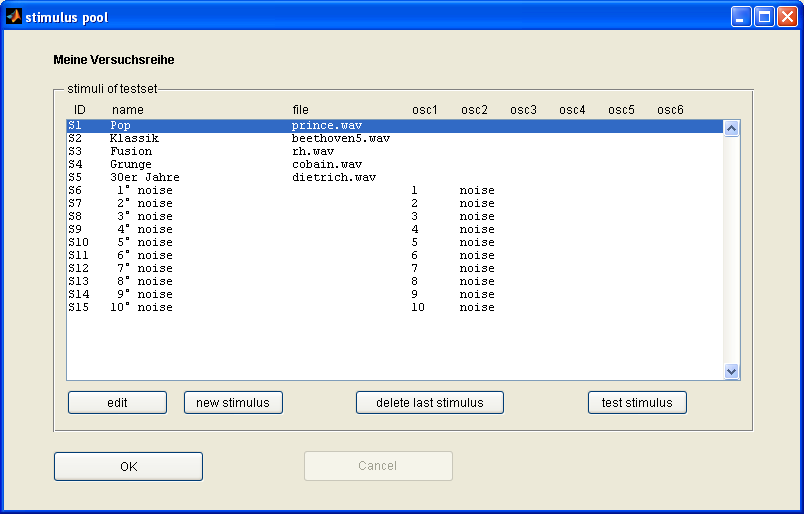
\includegraphics[resolution=150]{stimulus_pool.png}
%  	\caption{DW	 \textit{stimulus pool}}
%  	\label{fig:stimulus_pool}
%\end{figure}
\begin{figure}[h]\centering
	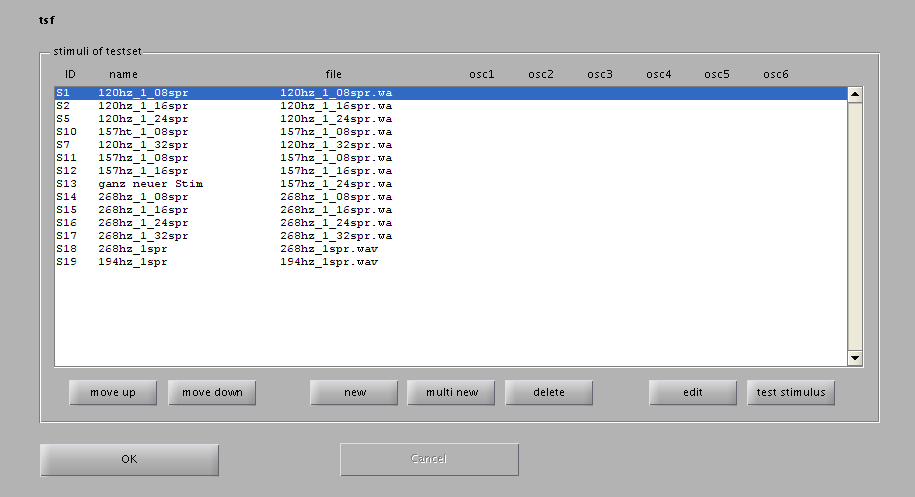
\includegraphics[resolution=150]{stimulus_pool_neu.png}
  	\caption{DW	 \textit{stimulus pool}}
  	\label{fig:stimulus_pool}
\end{figure}

Before stimuli can be chosen for application in certain test procedures, they have to be defined on a global level. For this purpose use the button \textit{stimulus pool} (see sec.~\ref{desktop}) or the item \textit{edit\textbackslash stimulus pool} from the menu bar (see sec.~\ref{menubar}) to access a DW labelled as \textit{stimulus pool} (see fig.~\ref{fig:stimulus_pool}), which contains a list providing an overview on the stimuli which have been defined already and their belonging playback properties. The supplied information for each stimulus consists of an automatically generated \textit{ID}, a user-defined label (\textit{name}), if applicable the name of a \textit{.wav} file or a set of \textit{OSC commands} or both. 

New stimuli can be added by using the button \textit{new}  or \textit{multi new}. While the former will only generate an empty stimulus in the list which later will have to be edited in order to be useful, the latter will open a file selection dialog window allowing multiple selection of .wav files. For each .wav file selected a separate stimulus associated with that .wav file will be added to the list \footnote{For techniques of economically configuring multiple OSC stimuli instead please cf.\,sec.~\ref{defaults_presets}.}. Names will be auto-generated from the file names, but of course can be edited later\footnote{Auto-generation of names from file names will be suspended however, if the default stimulus name has been changed, cf.\,sec.~\ref{defaults_presets}.}.

Unwanted stimuli can be deleted by using the  \textit{delete} button \footnote{While it is possible to delete global stimuli which have been assigned inside procedures (see sec.~\ref{testprocedures}), you are highly encouraged to follow good practice and separate global stimulus setup from procedure stimulus assignment and first perform the one, afterwards the other.}.  

Stimuli can be sorted using the  \textit{move up} and  \textit{move down} button, and the order the stimuli are in here will be the order the stimuli will be presented to you in all the other DWs when there are stimuli to be selected from the global stimulus pool.

 If one wants to test if a selected stimulus' properties (see below) have been set well, one can use the button \textit{test stimulus} for a presentation of it on a trial basis.

The editing of a stimulus' properties is performed by selecting the concerning position of the list and then using the \textit{edit} button, which will open a suitable DW labeled as \textit{edit stimulus} whose control elements will be described below. On this window definitions can be made regarding the stimulus' label (\textit{name}), duration and content. The latter can be chosen either as a .wav file or a set of up to 6 OSC commands or even both at a time. That means that both kinds of playback environment, auditory and visual, can be addressed. If you choose a .wav file from any location of your data drive, it will be copied to the folder \textit{audiofiles}, which is a sub folder of the \textit{test series} folder (see sec.~\ref{testseries}). The idea behind this behavior is to be able to easily transfer a test series' configuration data set between computers with a minimum amount of adjustments necessary. One restriction resulting from this is that the name of a chosen .wav file must be unique and not allocated to several files. When uploading a .wav file the stimulus' duration will be automatically determined as the file's length. The stimulus' name will also be auto-generated \footnote{This does \textit{not} apply if the name has previously been altered from the default! Cf.\,also sec.~\ref{defaults_presets}}. If playback of stimuli is triggered/involves additional via OSC commands, the stimulus' duration should be edited or must be manually entered respectively (the latter is the case if no .wav file is chosen). This is necessary because the software will receive no feedback information about the termination of playbacks controlled by OSC. As a consequence the entered duration period has to be long enough to include all presentations of the different contents, i.e. possibly a combination of a .wav file and several OSC commands to be executed at a time.


\begin{figure}[h]\centering
	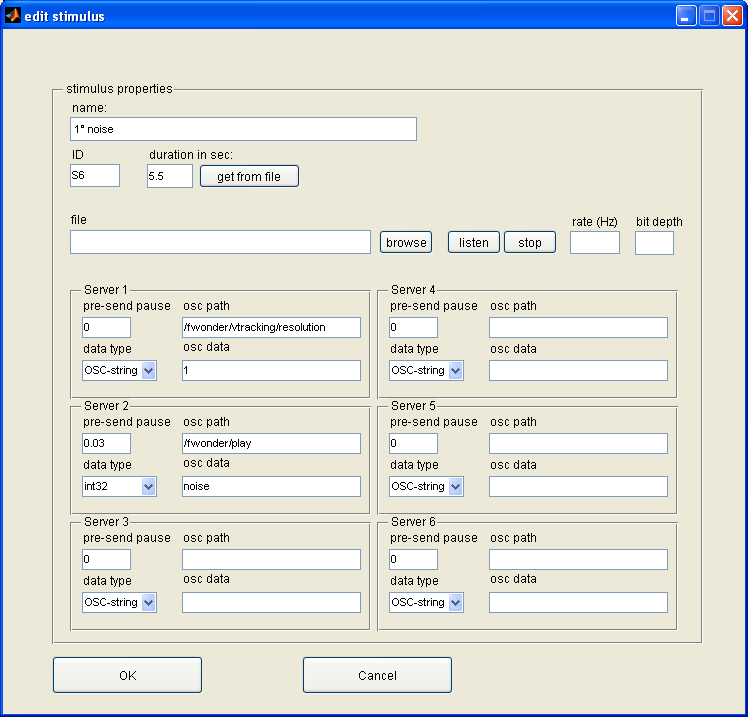
\includegraphics[resolution=150]{edit_stimulus.png}
  	\caption{DW	 \textit{edit stimulus}}
  	\label{fig:edit_stimulus}
\end{figure}

\newpage
\minisec{DW \itshape\lqq edit stimulus\rqq}\medskip
\begin{description}
	\item[stimulus properties] (\textit{panel})\hfill
	\begin{description}
		\item[name] (\textit{input field}) Space for entering the name or a short description of the stimulus respectively. The input will be treated as a string. This should release the user from distinguishing the selected stimulus from the remaining ones during the process of setting up test procedures. If this field has not yet been altered from the initial default and you select a .wav file by way of the appropriate dialog, this field will be auto-filled with a name generated from the .wav file minus its extension. Which name is displayed here upon stimulus creation as a default name can also be manipulated, cf.\,sec.~\ref{defaults_presets}.
		\item[ID] (\textit{output field}) Displays the stimulus' ID.
		\item[duration in sec] (\textit{input/output field}) In this field either the duration of the stimulus in [sec] can be manually entered or will displayed when received by using the \textit{get from file} button.
		\item[get from file] (\textit{button}) Obtains the stimulus duration from a .wav file if there has been one already specified in the \textit{file} field.
		\item[file] (\textit{input/output field}) In this field the original path of a .wav file which shall be played back directly from the sound card as part of the stimulus' audio content, either will be manually entered or displayed if received by using the file dialog which can be accessed by using the \textit{browse} button. 
		\item[browse] (\textit{button}) Opens a file dialog for selecting the path of a .wav file which shall be played back directly from the sound card as part of the stimulus' audio content. When leaving the current DW (\textit{stimulus properties}) and confirming changes by pressing the \textit{OK} button, the selected file will be copied to the folder \textit{audiofiles} which is a subfolder of the \textit{test series} folder (see sec.~\ref{testseries}). After this the \textit{file} field will no longer contain the path but only the file's name.
		\item[listen] (\textit{button}) Plays the .wav file if one has been specified. This function can be used for identification and calibration purposes.
		\item[stop] (\textit{button}) Stops the .wav file's playback.
		\item[{rate [Hz]}] (\textit{output field}) Displays the sampling rate in [Hz] if a .wav file has been specified.
		\item[bit depth] (\textit{output field}) Displays the resolution of the quantization process in [bit] if a .wav file has been specified.
		\item[Server 1--6] (\textit{panel}) Here a set of up to 6 OSC commands can be determined with each addressing one of up to 6 servers which have to be specified globally (see sec.~\ref{basic_network}). The commands will be executed in sequence with the order given by their ascending label numbers. 
		\begin{description}
			\item[pre-send pause] (\textit{input field}) Space for entering a time period in [sec] that lies between the previous and the current command's execution.
			\item[osc path] (\textit{input field}) Space for entering the path of the parameter one wants to address.
			\item[data type] (\textit{drop-down list}) Here one can choose among five types of data formats which are \textit{OSC-string}\footnote{A sequence of ASCII coded characters terminated by zero (C-String), filled up with zeros to a length of an integer multiple of four.}, \textit{int32}, \textit{float32}, \textit{True} and \textit{False}. For a description of these the user is directed to e.g. \citet{osc}.
			\item[osc data] (\textit{input field}) Space for entering the data of the format which has been previously specified. This field will be disabled if either \textit{True} or \textit{False} are selected.
		\end{description}
	\end{description} 
\end{description}


\section{Third Step: Configuration of Session Setup}\label{sessions_setup}
In order to be able to perform and control different test runs under several experimental conditions within one test series (cp. sec.~\ref{concept}), a structural variable called \textit{session} has been defined. Each subset of runs under one equally determined set of experimental conditions is thereby attached to a specific value of this variable. The variable's range starts at 1 and extends by integer steps to its maximum which is called \textit{number of sessions}. Before the different experimental conditions can be specified for each test section, the number of sessions has to be determined as a global parameter. This can be done by using the button \textit{session setup} placed on the main windows' s desktop (see. sec.~\ref{desktop}) or selecting the item \textit{edit\textbackslash session setup} from the menu bar (see sec.~\ref{menubar}). Thereupon a suitable DW will open. By default the number of sessions is set to 1.


\section{Fourth Step: Specification of Test Sections}\label{edit_testsections}
As mentioned in sec.~\ref{concept} \whisper\ allows to sequentially perform several sub-tests within one test run. For this reason there may be several \textit{test sections} assigned to a single test run. Moreover for each test section one must select an appropriate test procedure. Both tasks can be carried out by either using the button \textit{edit test sections} which is placed on the main window's desktop or selecting the item \textit{edit\textbackslash test sections} from the menu bar. In both cases a DW appears which is labelled as \textit{edit test sections} and whose control elements are described in the following.

\begin{figure}[h]\centering
	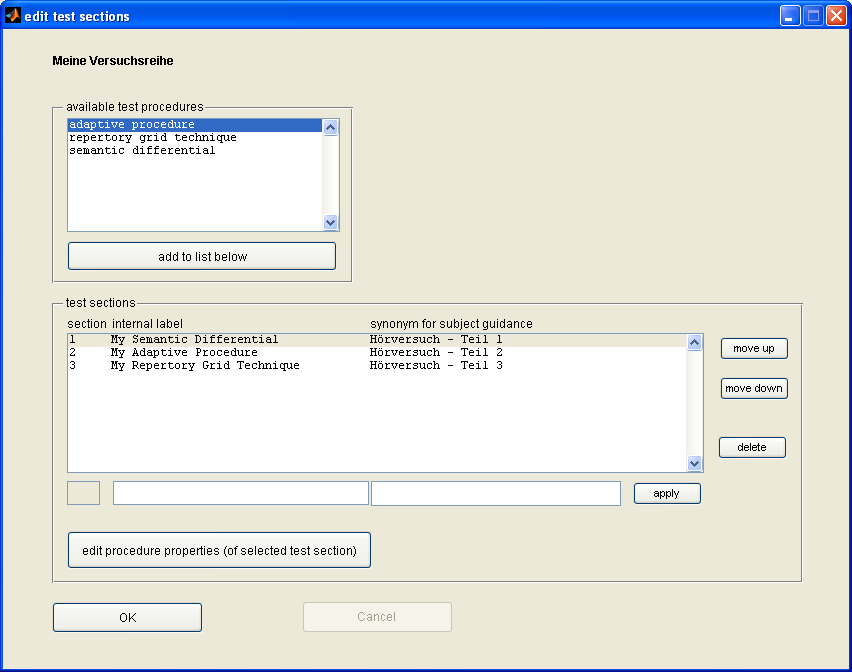
\includegraphics[resolution=150]{edit_testsections.png}
  	\caption{DW \textit{edit test sections}.}
  	\label{fig:edit_testsections}
\end{figure}

\minisec{DW \itshape\lqq edit test sections\rqq}\medskip
\begin{description}
	\item[available test procedures] (\textit{panel})\hfill
	\begin{description}
		\item[\textrm{\textless}no label\textrm{\textgreater}] (\textit{list box}) Shows all test procedures available under \whisper.
		\item[add to list below] (\textit{button}) Adds a selected test procedure to the bottom of the list of \textit{test sections} below. 
	\end{description}
	\item[test sections] (\textit{panel})\hfill
	\begin{description}
		\item[\textrm{\textless}no label\textrm{\textgreater}] (\textit{multi-columned list box}) Shows all test sections in an order defined by the user. The entries of the three columns represent the count number, an internal label which should support identification by the user (i.e. the experimenter) and a synonym which will be used for subject guidance during a test run.
		\item[\textrm{\textless}no label\textrm{\textgreater}] (\textit{output field} 1st col) Shows the count number of the selected test section.
		\item[\textrm{\textless}no label\textrm{\textgreater}] (\textit{input/output fields} 2nd \& 3rd col) Space for displaying and editing of both the labels for the experimenter and the subject belonging to the selected test section.
		\item[apply] (\textit{button}) Applies changes in the contents of the input/output fields above to the selected test section.
		\item[delete] (\textit{button}) Deletes a selected test section.
		\item[move up/move down] (\textit{button}) Shifts the selected test section to a proximate list position above/below.
		\item[specify test properties] (\textit{button}) Opens a DW for determining the properties of the test procedure that is chosen for the selected test section (cp. sec.~\ref{procedure_parameters}).
	\end{description}
\end{description}


\section{Fifth Step: Setting up Procedure Properties}\label{procedure_parameters}
The process of determining a specific test procedure's properties is triggered by applying the button \textit{specify test properties} from the DW \textit{edit test sections} which has been described in sec.~\ref{edit_testsections}. Then a DW labeled as \textit{\textless abbreviatory denotation of the type of test procedure\textgreater\ --~main settings (\textless internal label of the current test section\textgreater)} will open which has different appearances in dependency on the type of test procedure that has been addressed to the currently selected test section. This window and the further approach to setting up the properties will be described in chapter \ref{testprocedures}, to be more precise in the respective subsection belonging to the regarding test procedure.





%-----------------------------------------
% CHAPTER 6
%-----------------------------------------

\chapter{Performing a Test Run}\label{testrun}


\section{Initializing and Starting a Test Run}\label{start_testrun}
Right before a test run's performance only a few parameters have to be set by the experimenter. This is done on the panel \textit{next test run} which is placed on the main window's desktop (see. sec.~\ref{desktop}). The basic run parameter settings refer to the specification of the subject's ID and the input of the session key which is associated with certain experimental conditions (cp. sec.~\ref{sessions_setup}). Both actions have to be performed in the sub-panel \textit{run parameters}. Furthermore one can choose only to perform a subset of test sections by making a selection using the sub-panel \textit{execution of test sections}. The test run is started by actuating the button \textit{Start run}. After this the GUI system for the subject's guidance and the collection of the data appears which will be described in the following section.


\section{The Test Subject's GUI System}\label{sub_guisystem1}

\begin{figure}[h]\centering
	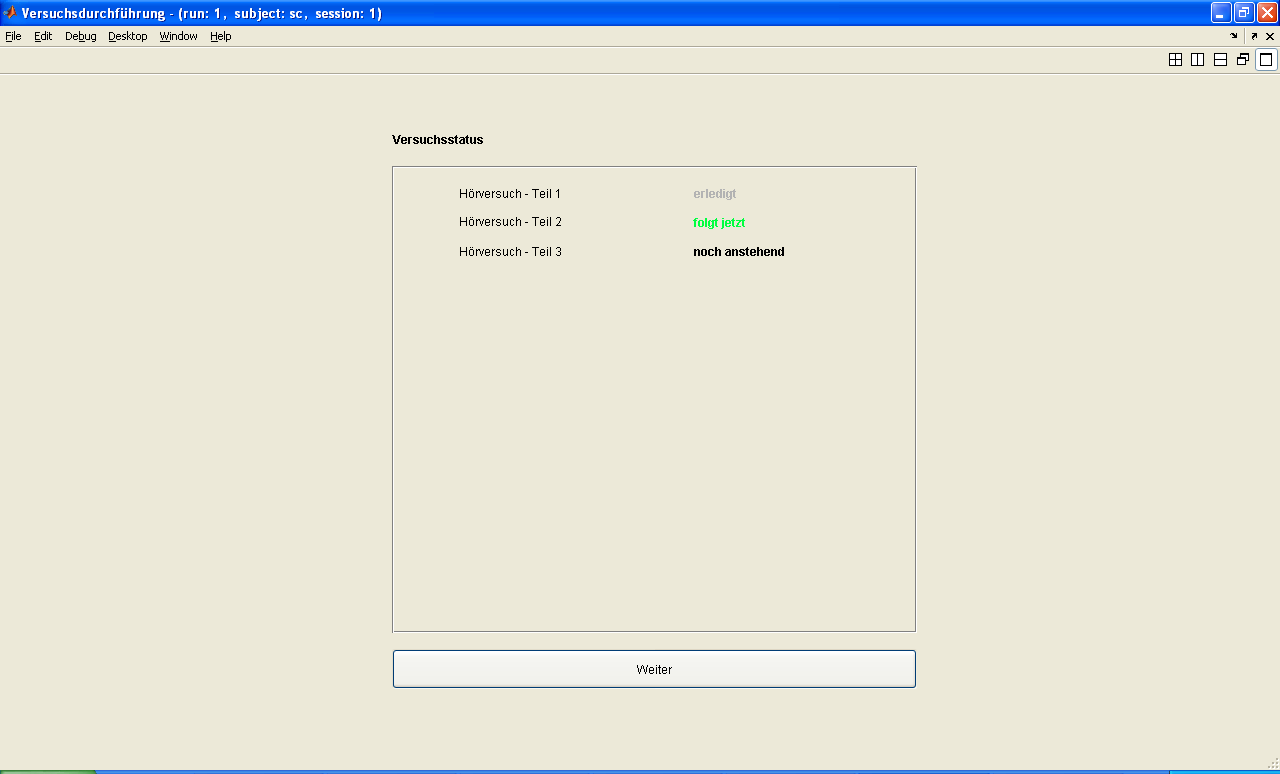
\includegraphics[width=\textwidth]{subject_screen1}
  	\caption{GUI system for subject guidance -- basic screen showing information on the test run's status of progression.}
  	\label{fig:subject_screen1}
\end{figure}

The basis of the subject's GUI system is constituted by a window which is maximized to cover the whole screen and which stays in the background during the whole test run's performance. This window is labeled as \textit{Versuchsdurchfuehrung} (German for "Test Execution"). 
\\
\\
\textbf{In \whisper\ most test information on the subject side (besides self-definable instruction texts) will be presented in German language. If this needs to be changed, one has to modify the source code and is therefore directed to the technical documentation (see sec.~\ref{doc}).} 
\\
\\
In the following this window will be called the subject's \textit{basic screen}. It will alternatively display the test run's current state of progress, or instructions for subjects. The test's progress is signaled at the beginning of a run and after each test section by displaying a list of the individual test names as defined by the experimenter beforehand (see sec.~\ref{edit_testsections}). Thereby, names representing completed test sections are shown in grey letters, the upcoming test is displayed in green an all remaining ones in black (see fig.~\ref{fig:subject_screen1}). After clicking the \textit{Weiter} ('Continue') button, the initial test instructions will be displayed (see fig.~\ref{fig:subject_screen2}). Instructions may be freely defined by the experimenter beforehand when specifying a procedure's properties (see chap.~\ref{testprocedures}). After reading the instruction, the subject may click the \textit{OK} button and will then be presented with the current test procedures GUI. GUIs differ according to the type of test conducted; more details on these windows can be found in chapter~\ref{testprocedures}.

\begin{figure}[h]
	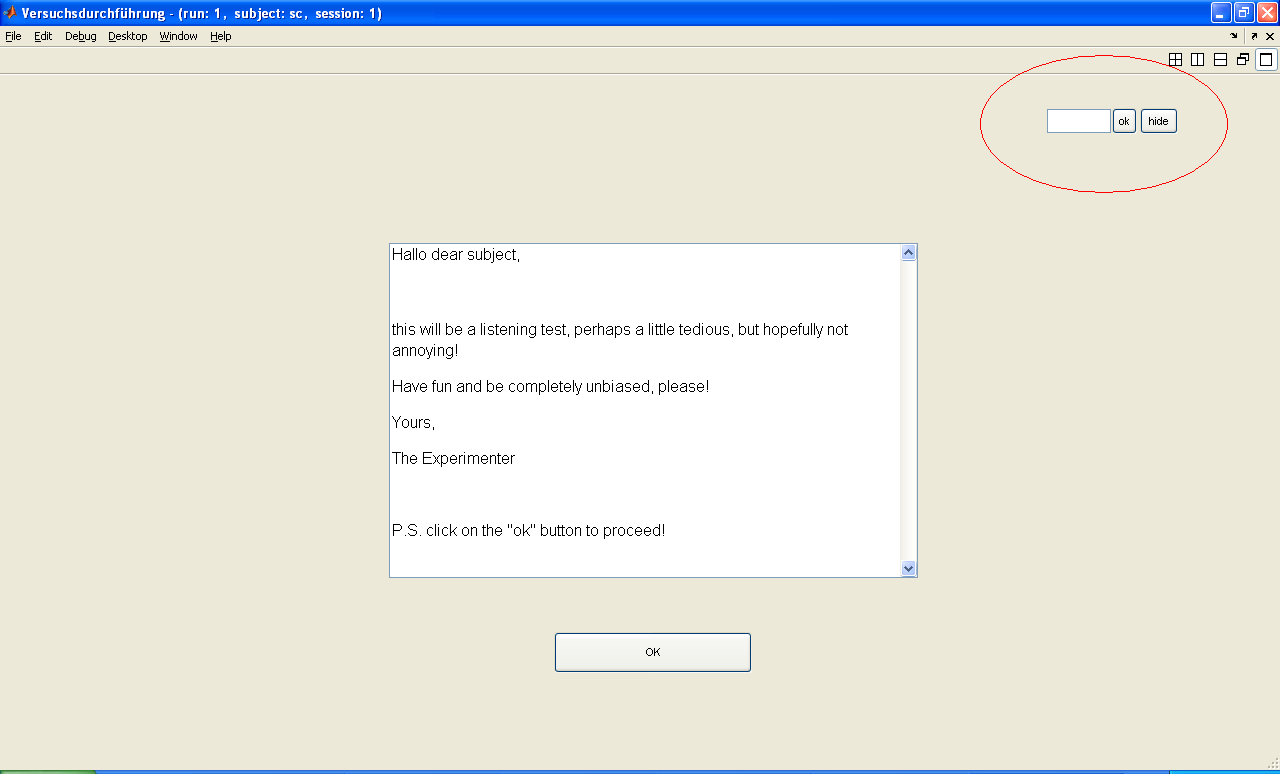
\includegraphics[width=\textwidth]{subject_screen2}
  	\caption[GUI system for subject guidance -- \textit{basic screen} showing the initial instructions.]{GUI system for subject guidance -- \textit{basic screen} showing the initial instructions. \textbf{IMPORTANT NOTE: The top right corner of the GUI shows a -- normally hidden -- input field appearing only, if one actuates the window's 'close' icon. When entering the word \lqq break\rqq\ one may stop (break) the current test and return to the program's main window.}}
  	\label{fig:subject_screen2}
\end{figure}


The subject's basic screen will stay maximized in the background during a test run. To avoid false aborts caused by subjects the 'close' icons of all windows belonging to the subject's GUI system have been disabled. If it is required to break a test run in a controlled way, the experimenter may click on the standard \textit{close} icon at the right corner on the subject's basic window. This will open a text input field (see fig.~\ref{fig:subject_screen2}) for entering the word \lqq break\rqq. Clicking \textit{ok} will then close the subject's GUI system and return the user to the program's \textit{main window}. \textbf{In such a case the inclusion of the empirical data collected up to this point into the test series's data set might be unwanted. Therefore, one may delete the data of the last test run by using the menu item \textit{edit\textbackslash empirical data} (see sec.~\ref{menubar}).}





%-----------------------------------------
% CHAPTER 7
%-----------------------------------------

\chapter{Test Procedures -- Configuration and Execution}\label{testprocedures}


\section{Adaptive Psychophysical Threshold Procedures (AP)}
\subsection{The Test Run}\label{ap_run}

\begin{figure}[h]\centering
	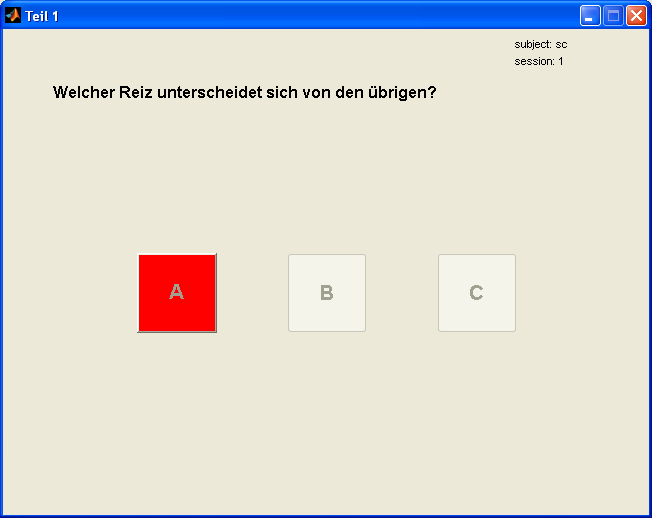
\includegraphics[resolution = 150]{ap_subject.png}
 		\caption{The subject's GUI when conducting an adaptive psychophysical threshold procedure.}
  	\label{fig:ap_subject}
\end{figure}

The design of the GUI for collecting the subject's responses depends on the selected response paradigm. At the program's current state one may apply nAFC-paradigms with $n=2, 3 \ or \ 4$. Figure~\ref{fig:ap_subject} shows the interface for a presentation of three stimulus intervals. The interface generally comprises $n$ squared icons arranged on a horizontal line representing the stimulus intervals. The first stimulus' playback  starts automatically at the beginning of a trial. To allow for a short delay the experimenter can determine a suitable time period (see sec.~\ref{ap_setup}). A further period of silence can be defined for in between the presentations of the stimulus intervals. During the playback the respective icon which carries the current interval's number is highlighted to supply the subject visual information which should help assigning the current perception to the correct interval. After all stimuli of one trial have been played, the subject selects the intervals which it supposes to represent the deviant (target) stimulus by clicking on the respective icon. At the same time the procedure will proceed with presenting the next trial. 

The current target stimulus' characteristic is controlled by an adaptation mechanism which one may chose from a larger collection being shortly described already in section~\ref{sec:testprocedures}. A singular test section may contain either a single adaptive track, or an arbitrary number of interleaved tracks which use the same response paradigm.

\subsection{Setting up Properties}\label{ap_setup}
The configuration of an adaptive procedure can be divided into several hierarchical \lqq layers\rqq\ implying a stepwise setup action. This is due to some of the properties being set on lower \lqq layers\rqq\ are affected by those defined on higher ones, whereas the reversed case does not appear. 
\\
The top \lqq layer's\rqq\ settings refer to the response paradigm, the time period between trials, terms of instructions and the laying of the tracks one wants to run. These settings are performed on the DW \textit{AP -- main settings (...)} (see fig.~\ref{fig:ap_main_settings}) which can be accessed as explained in subsection \ref{procedure_parameters} and will be described below. If several tracks have been created, one may either randomly interleave all these tracks or define subsets of tracks which are then assigned to different sessions. If a subset comprises more than one track, these tracks will be randomly interleaved. 
\\
By selecting a single track from the respective list-box and actuating the \textit{edit} button, one gets to the DW \textit{AP -- track settings (...)} (see fig.~\ref{fig:ap_track_settings}) which represents the next lower \lqq layer\rqq\ which is for determination of the track's settings. These include specifying a label, setting the range of stimulus intensities, assigning the stimuli from the stimulus pool to the single intensity values and choosing the desired adaption and estimation mechanism out of five categories --~Staircase, PEST, ZEST, QUEST and (manually configured) ML/Bayesian procedure. By clicking on the \textit{settings} button belonging to the selected mechanism, one arrives at the third \lqq layer\rqq, which refers to the mechanism's parameters. Setting up those will be described in the regarding paragraphs below. But before, there will be given a description of the DWs referring to the first two \lqq layers\rqq.

\begin{figure}[h]\centering
	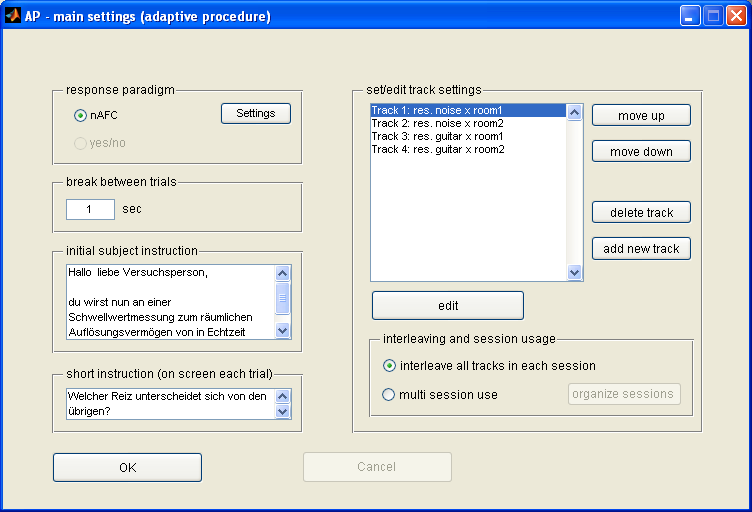
\includegraphics[resolution = 150]{ap_main_settings.png}
 		\caption{DW \textit{AP -- main settings (...)}}
  	\label{fig:ap_main_settings}
\end{figure}

\minisec{DW \itshape\lqq AP -- main settings (...)\rqq}\medskip
\begin{description}
	\item[response paradigm] (\textit{panel})\hfill
	\begin{description}
		\item[nAFC] (\textit{radio button}) If selected: selection of the nAFC paradigm.
		\item[yes/no] (\textit{radio button}) \textless this option is not available at the program's current state\textgreater
    \item[settings] (\textit{button}) Opens a window for specification of the response paradigm's settings. For the nAFC paradigm these are the number $n$ of stimulus intervals, which can either be $2, \, 3 \, or \, 4$ (default: 3) and the time period of silence between the intervals in seconds (default: 1~sec). Moreover it can be specified, wether or not the subject is allowed to listen to the stimuli as often as she/he wants.
	\end{description}
	\item[break between trials] (\textit{panel})\hfill
	\begin{description}
		\item[\textrm{\textless}no label\textrm{\textgreater}] (\textit{input field}) Space for entering the time period in seconds that lies between the subject's response and the initiation of the next trial's first stimulus' playback (default: 2~sec). The input will be treated as a double value.
	\end{description}
	\item[initial subject instruction] (\textit{panel})\hfill
	\begin{description} 
		\item[\textrm{\textless}no label\textrm{\textgreater}] (\textit{multi-lined input field}) Space for entering terms of instructions that will be displayed on the subject's \textit{basic screen} (see sec.~\ref{testrun}) before the current test section is started.
	\end{description}
	\item[short instruction (on screen each trial)] (\textit{panel})\hfill
	\begin{description} 
		\item[\textrm{\textless}no label\textrm{\textgreater}] (\textit{input field}) Space for entering a short term of instruction that will be displayed on top of the subject's user interface in each trial.
	\end{description}
	\item[set/edit track settings] (\textit{panel})\hfill
	\begin{description} 
		\item[\textrm{\textless}no label\textrm{\textgreater}] (\textit{multi-columned list box}) This list shows all the tracks that have been defined within the selected test section and across all sessions.  The first column views the track number and the second its label name. Thereby a track's number is only important for its identification. Just for reasons of clearness there exists the possibility to shift a selected track to another list position by using the \textit{move up/down} buttons (see below). 
		\item[edit] (\textit{button}) Opens a DW labeled as \textit{AP -- track settings (...)} and described below, for the specification of properties like the track's label name, the definition of the stimulus intensity's range and the choice of an appropriate adaption and estimation mechanism. 
		\item[move up/down] (\textit{button}) Shifts the selected item (i.e. track) to a proximate list position above/below.
		\item[delete track] (\textit{button}) Deletes the selected item (i.e. track).
		\item[add new track] (\textit{button}) Adds a new item (i.e. track) to the list's end.
		\item[interleaving and session usage] (\textit{sub-panel})\hfill
		\begin{description}
			\item[interleave all tracks in each session](\textit{radio button}) If selected, all defined tracks will be performed across all (globally) defined (cp. sec.~\ref{sessions_setup}) sessions in an randomly interleaved manner. \textit{Note:} If the list consists of only one item (which is supposed to be a rather common scenario), this single track will be performed in the \lqq normal\rqq\ (i.e. non-interleaved) manner (across all defined sessions).
			\item[multi session use](\textit{radio button}) If selected, in each run a subset of tracks which has been defined by the experimenter and assigned to a certain session key number, will be performed in a randomly interleaved manner (exclusively within the respective session). \textit{Note:} If a subset consists only of one track, this single track will be performed in the \lqq normal\rqq\ (i.e. non-interleaved) manner (within the belonging session).
			\item[organize sessions](\textit{button}) If the respective option has been chosen, this button opens a DW that allows for defining subsets of tracks with each of them assigned to a certain session.
		\end{description}
	\end{description}
\end{description}

\begin{figure}[h]\centering
	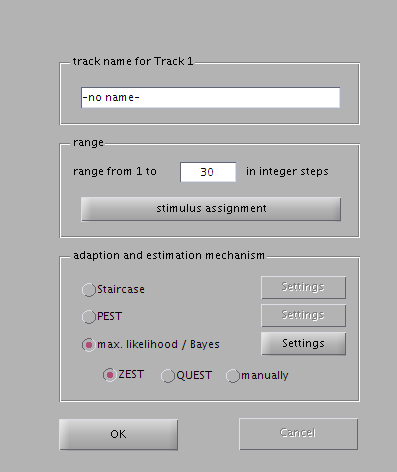
\includegraphics[resolution = 150]{ap_track_settings_new.png}
 		\caption{DW \textit{AP -- track settings (...)}}
  	\label{fig:ap_track_settings}
\end{figure}

\minisec{DW \itshape\lqq AP -- track settings (...)\rqq}\medskip
\begin{description}
	\item[track name for Track \textrm{\textless}no. of selected track\textrm{\textgreater}] (\textit{panel})\hfill
	\begin{description}
		\item[\textrm{\textless}no label\textrm{\textgreater}] (\textit{input field}) Space for determining a label name for the selected track.
	\end{description}
	\item[range] (\textit{panel})\hfill
	\begin{description}
		\item[\textrm{\textless}no label\textrm{\textgreater}] (\textit{input field}) Space for entering the maximum stimulus intensity\footnote{For simplification this parameter by itself sometimes is called \textit{Range}. Note that this denotation will appear in some of the following statements and formulas.} which has to be an integer value greater than 1. The stimulus intensity's range then is defined from 1 to this value in steps of 1. \textit{Note:} Usually stimulus intensities are scaled in a specific unit and one wants to realize a different resolution than integer steps. In this (normal) case one has to apply a transformation to the physical domain outside the software with the discrete values kept in a look up table. Basically stimulus intensities should be \lqq chosen along some scale that yields approximately equal sensory intervals\rqq\ \citep{cornsweet:1962}. At least for the application of parametric methods (e.g. in ML/Bayesian procedures) a certain shape of the psychometric function is assumed \citetext{\citealp{treutwein:1995}}. \textit{Further note:} This parameter affects some properties of lower configuration layers, i.e. several of those that depend on the range, e.g. the signals assigned to the stimuli and properties of the selected adaption and estimation mechanism such as initial values, position and shape parameters, etc.. So if this parameter's value will be changed after the mechanism's properties have already been set, some of the latter could be changed or overwritten by default values. It is therefore strongly recommended that in this case one repeatedly checks these properties to be on the safe side.
		\item[stimulus assignment] (\textit{button}) Opens a DW for assigning the stimulus signals from the stimulus pool to the discrete integer values of stimulus intensities. This includes a reference stimulus for which also an intensity value can be specified, which has rather to be seen as a label and won`t be used by the program at the current state for any calculation, but might be helpful for documentation and evaluation purposes.
	\end{description}
	\item[Adaption and estimation mechanism] (\textit{panel})\hfill
	\begin{description} 
		\item[Staircase] (\textit{radio button}) Selection of the \textit{Staircase} procedure for placing stimuli and the threshold's estimation.
		\item[PEST] (\textit{radio button}) Selection of the \textit{PEST} procedure for placing stimuli and the threshold's estimation.
		\item[max. likelihood/Bayes] (\textit{radio button}) Selection of \textit{ML/Bayesian} procedures, based on the Best-PEST but including extensions taken from several similar procedures; selecting this enables the selection of one of the following three choices:
                  \begin{description}
                        \item[ZEST] (\textit{radio button}) Selection of the \textit{ZEST} procedure for placing stimuli and the threshold's estimation; this preselects the appropriate options of the ML/Bayes based procedures for ZEST and disables the  others.
                        \item[QUEST] (\textit{radio button}) Selection of the \textit{QUEST} procedure for placing stimuli and the threshold's estimation. This preselects the appropriate options of the ML/Bayes based procedures for QUEST and disables the  others.
                        \item[manually] (\textit{radio button}) Selection of \textit{ML/Bayes} procedures for placing stimuli and the threshold's estimation; options from all extensions implemented in \whisper\ are available to the user (yet no obvious guidance how to sensibly combine them).
                  \end{description}
		\item[settings] (\textit{button} (3x)) Opens a DW for specifications on the selected mechanism, labelled as \textit{AP -- edit \textless selected type of adaptive procedure\textgreater\ settings (...)} (see below).
	\end{description}
\end{description}


\subsubsection{Staircase}

\begin{figure}[h]\centering
	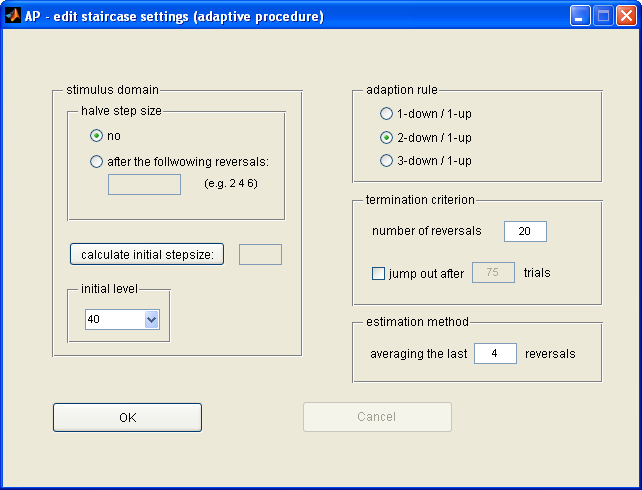
\includegraphics[resolution = 150]{ap_edit_staircase_settings.png}
 		\caption{DW \textit{AP -- edit staircase settings (...)}}
  	\label{fig:ap_edit_staircase_settings}
\end{figure}

\minisec{DW \itshape\lqq AP -- edit staircase settings (...)\rqq}\medskip
\begin{description}
	\item[stimulus domain] (\textit{panel})\hfill
	\begin{description}
		\item[halve step size] (\textit{sub-panel})\hfill
		\begin{description}
			\item[no] (\textit{radio button}) If selected, there will be no decrease of step size during a run.
    	\item[after the following reversals] (\textit{radio button}) If selected, the step size will be halved after a set of reversals which has been determined by the experimenter.
    	\item[\textrm{\textless}no label\textrm{\textgreater}] (\textit{input field}) Space for entering a set of numbers defining the track's reversals at which the step size should be halved. The single values should be integers greater than 1 and at most equal to the maximum number of reversals to be performed (see panel \textit{termination criterion}). Each value must appear only once. The items have to be separated by space. Let's say one wants to achieve bisections after the 2., 4. and 6. reversal appearing during the run. Then one has to enter \lqq 2 4 6\rqq. \textit{Note:} Be careful not to insert a space after the last item!
    \end{description}
    \item[calculate initial step size:] (\textit{button}) Calculates the size of the first step. This value directly depends on the number of bisections defined before. For example if one has chosen the reversals 2, 4, and 6 for halving the step size, the initial step size will be 8, as the minimum step size is always 1. \textit{Note:} This function has no direct effect on the algorithm underlying the procedure. Its purpose only is to facilitate the configuration process. It should prevent the experimenter from defining too many bisections which might result in an absurd initial step size that is comparable to or even exceeds the range. 
    \item[\textrm{\textless}no label\textrm{\textgreater}] (\textit{output field}) Space for viewing the initial step size's value which is calculated after actuating the respective button (see above).
    \item[initial level](\textit{sub-panel})\hfill
    \begin{description}
    	\item[\textrm{\textless}no label\textrm{\textgreater}](\textit{drop-down list}) Here the initial value of the stimulus intensity can be selected. By default this is set to the range's maximum value.
    \end{description}
	\end{description}
	\item[adaption rule] (\textit{panel})\hfill
	\begin{description}
		\item[1-down/1-up] (\textit{radio button}) If selected, a simple 1-down/1-up adaption rule will be applied.
		\item[2-down/1-up] (\textit{radio button}) If selected, a transformed 2-down/1-up adaption rule will be applied.
		\item[3-down/1-up] (\textit{radio button}) If selected, a transformed 3-down/1-up adaption rule will be applied.
	\end{description}
	\item[termination criterion] (\textit{panel})\hfill
	\begin{description} 
		\item[number of reversals] (\textit{input field}) Space for entering the maximum number of reversals which will be performed and after that the procedure will be terminated.
		\item[jump out after ... trials] (\textit{check box \& input field}) If the box is checked, one may specify a maximum number of trials that will be performed and after that the procedure will be terminated if the maximum number of reversals has not been reached yet. \textit{Note:} This additional termination criterion was installed in order to avoid unreasonably long trial sequences. If this criterion catches and the first does not, the threshold's estimate will not be calculated as the estimation method (see panel below) then cannot be applied. In this case 0 is returned as the output. (Under certain conditions the calculation of a threshold estimate might be caught up manually outside the program by applying a slightly different scheme, e.g. using previous reversals for averaging stimulus intensities.)
	\end{description}
	\item[estimation method] (\textit{panel})\hfill
	\begin{description} 
		\item[averaging the last ... reversals] (\textit{check box \& input field}) Space for entering the number of last consecutive reversals whose associated stimulus intensities will be averaged for calculating the threshold's estimate. \textit{Note:} T\textbf{his number must not exceed the track's maximum number of reversals specified before (see panel \textit{termination criterion}). Otherwise the algorithm will not work properly.} From a methodical point of view, i.e. in order to maximize accuracy and minimize bias, averaging should only cover an even number of reversals including only those that appear after the minimum step size has already been reached.
	\end{description}
\end{description}


\subsubsection{PEST}

\begin{figure}[h]\centering
	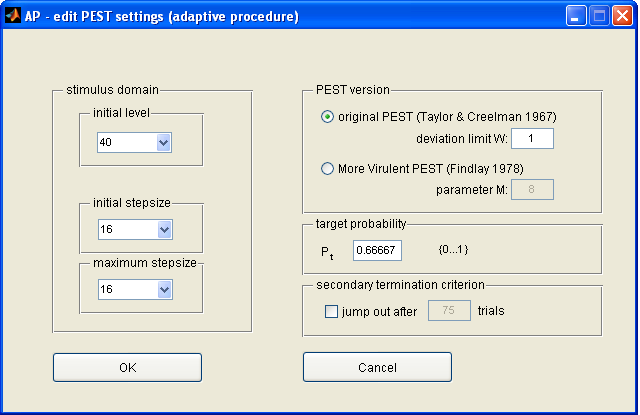
\includegraphics[resolution = 150]{ap_edit_pest_settings.png}
 		\caption{DW \textit{AP -- edit PEST settings (...)}}
  	\label{fig:ap_edit_pest_settings}
\end{figure}

\minisec{DW \itshape\lqq AP -- edit PEST settings (...)\rqq}\medskip
\begin{description}
	\item[stimulus domain] (\textit{panel})\hfill
	\begin{description}
		\item[initial level] (\textit{sub-panel})\hfill
		\begin{description}
			\item[\textrm{\textless}no label\textrm{\textgreater}] (\textit{drop-down list}) Here the initial value of the stimulus intensity can be selected. By default this is set to the range's maximum value.
    \end{description}
    \item[initial step size] (\textit{sub-panel})\hfill
		\begin{description}
			\item[\textrm{\textless}no label\textrm{\textgreater}] (\textit{drop-down list}) Here the size of the first step can be selected. By default this is the second largest value that is possible in the case, i.e. the second largest power of two that fits in the range.
			 \end{description}
    \item[maximum step size] (\textit{sub-panel})\hfill
		\begin{description}
			\item[\textrm{\textless}no label\textrm{\textgreater}] (\textit{drop-down list}) Here the maximum step size can be selected. This value will never be exceeded throughout the run no matter what value the rules call for. By default it is set to the second largest possible value, i.e. the second largest power of two that fits in the range. \textit{Note:} As this parameter already affects the first step, its value should be at least as high as the initial step size.
    \end{description}
	\end{description}\pagebreak[2]
  \item[PEST version] (\textit{panel})\hfill
  \begin{description}
    \item[original PEST (Taylor \& Creelman 1967)] (\textit{radio button}) If selected, the original PEST procedure described by Taylor \& Creelman \citep{taylor:1967} will be performed.
    \item[deviation limit W] (\textit{input field}) Space for entering the value of the parameter called \textit{deviation limit}. The authors of the PEST procedure suggest a value of $W=1$ if one wants to yield a target probability of $P_t=0.75$ and higher values like $W=1.5$ or $W=2$ for target probabilities closer to 0.5.
    \item[More Virulent PEST] (\textit{radio button}) If selected, a modified PEST procedure described by Findlay~(1978) \citep{findlay:1978} will be performed.
    \item[parameter M] (\textit{input field}) Space for entering the value of the parameter $M$. Sadly, the author gives no unambiguous recommendations on this parameter's choice. By default it is set to 8, as this is a moderate value used in the author's simulations.
  \end{description}
  \item[target probability](\textit{panel})\hfill
  \begin{description}
    \item[$P_t$](\textit{input field}) Space for entering the value of the target probability $P_t=\psi(\vartheta)$, i.e. the probability for a positive response at convergence. This value has to lie between 0 and 1 and should be chosen in dependency on the reponse paradigm. A reasonable choice is sometimes made by using Abott's formula (based on the classical threshold concept \citep[cp.][chap.~4]{gescheider}) to calculate the ordinate's value $\psi(x)$ of the psychometric function: 
		\begin{equation}\label{korrektur}
		\psi(x)=\gamma + \left[1-\gamma-\lambda\right] \cdot \psi^*(x)  
		\end{equation}
Thereby $\psi^*(x)$ is the probability of sensory discrimination, $\lambda$ is the lapsing rate and $\gamma$ the guessing rate or false alarm rate. At convergence $\psi^*(\vartheta)$ is usually defined as 50\%. In case of the nAFC paradigm there is $\gamma=\frac{1}{n}$. Hence by default the target probability is set to the respective value assuming $\lambda = 0$, i.e.
		\begin{equation}
		P_t=\frac{1}{n} + \left[ 1- \frac{1}{n} \right] \cdot 0.5
		\end{equation}
  \end{description}
  \item[secondary termination criterion](\textit{panel})\hfill
  \begin{description}
    \item[jump out after ... trials](\textit{check box \& input field}) If the box is checked, here one may enter the maximum number of trials that will be performed and after that the procedure will be terminated if this has not been done by the PEST rules yet. (The procedure regularly terminates when the minimum step size of 1 is under-run.) \textit{Note:} This additional termination criterion was installed in order to avoid unreasonably long trial sequences. If this criterion catches and the first does not, the threshold's final estimate cannot be properly calculated and is therefore set to 0. In this case one might want to look for the stimulus intensity that would have been taken for the next placement. This value can either be found in the log file (see sec.~\ref{logfiles}) or in the track's plot (see sec.~\ref{plots}). Note that this value comprises a different accuracy, as the minimum step size has not been under-run and possibly not even been reached yet.
    \end{description}
\end{description}
    

\subsubsection{ML/Bayesian procedure}\label{ml_bayesian}

\begin{center}%[h]\centering
	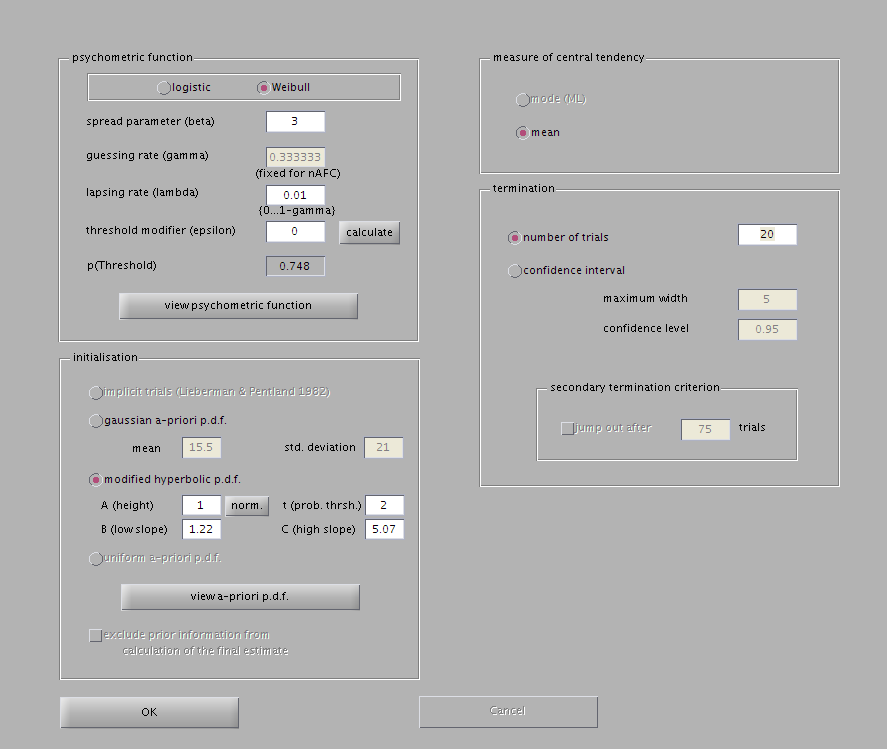
\includegraphics[resolution = 150]{ap_edit_mlbayes_settings2.png}
 		\captionof{figure}{DW \textit{AP -- edit ZEST settings (...)}}
  	\label{fig:ap_edit_mlbayes_settings}
\end{center}

\minisec{DW {\itshape\lqq AP -- edit ZEST settings (...)\rqq}\\
         DW {\itshape\lqq AP -- edit QUEST settings (...)\rqq}\\
         DW {\itshape\lqq AP -- edit ML/Bayes settings (...)\rqq}\footnote{This DW's title depends on your previous choice of ML/Bayes based procedures, cf.\,sec.~\ref{ap_setup}. The same goes for the availability of certain options of this DW.}}\medskip
\begin{description}
	\item[psychometric function] (\textit{panel})
	The shape of the underlying psychometric (model) function $\hat{\psi}(x)$ is described by one of the following two equations, which can be derived from equation~\eqref{korrektur} on page~\pageref{korrektur} by assuming a certain function  for $\psi^*(x)$.
        \begin{description}
              \item[logistic] (\textit{radio button}) The function used is the logistic function $\mathit{l}(x; \alpha , \beta)=\frac{1}{1+e^\frac{-(x-\alpha)}{\beta}}$. This yields:
	        \begin{equation}\label{psyfunc_logistic}
	          \hat{\psi}(x)=\hat{\psi}(x; \, \theta, \beta)=\gamma + \left(1-\gamma-\lambda\right) \cdot \frac{1}{1+e^\frac{-(x-\theta)}{\beta}}  
	        \end{equation}
	        Thereby $\lambda$ is the lapsing rate and $\gamma$ the guessing rate or false alarm rate which is assumed to be $\gamma = 1/n$ for the nAFC paradigm. $\theta$ is the unknown position parameter (which in case of a logistic model function is equal to the threshold) and $\beta$ the spread parameter (see further below). 
                \item[Weibull] (\textit{radio button}) The function used is the Weibull function\footnote{Used here in that of its many forms which is used by ZEST.}, yielding:
                  \begin{equation}\label{psyfunc_weibull}
                   \hat{\psi}(x)=\hat{\psi}(x; \, \theta, \beta)=\gamma + \left(1-\gamma-\lambda\right) \cdot exp[ -10^{ \beta ( x - \theta + \epsilon)}]
                \end{equation}
	        Again $\lambda$ is the lapsing rate, $\gamma$ the guessing rate (assumed to be $\gamma = 1/n$ for the nAFC paradigm), $\theta$ the threshold and $\beta$ the spread parameter. $\epsilon$ gives the possibility of shifting what point of the psychometric function is used as threshold, thereby influencing the threshold criterium (see below). 
Fields for input of  $\lambda$,  $\gamma$ and $\beta$ are "shared" with the fields for the corresponding input for the logistic function (see below).

Please note that one of the mandatory requirements for psychometric functions is that  for different conditions it doesn't change shape, but only its position along the x-axis, see e.\,g.\ \cite{watson:1983}. The Weibull function alas specifically meets this criterion only under the condition that the x-axis is scaled logarithmically, see e.\,g.\ \citetext{\citealp{treutwein:1995}}. Thus the Weibull function is best suited for use as psychometric function in those cases, where the relationship of the tested stimuli's intensities is logarithmic, too. 
\end{description}
	\begin{description}
		\item[spread parameter (beta)] (\textit{input field}) Space for entering the value of the spread parameter $\beta$ which should be chosen based on prior knowledge. Sometimes it might be helpful to consider its relationship to the psychometric function's slope $S$:
	\begin{equation}\label{slope}
	S = \frac{(1-\gamma-\lambda)}{4 \beta}.
	\end{equation}
	In other cases one might note the relationship to the spread $\sigma_l$ of the logistic function $l$, which is approximately given by
	\begin{equation}
	\sigma_l \approx 1.81 \cdot \beta
	\end{equation}
	\citep{hastings}.	If one has prior knowledge about a psychometric function being described by a cumulative normal ogive then one might use the relationship
	\begin{equation}
	\sigma_N \approx 1.7 \cdot \beta
	\end{equation}
	 with $\sigma_N$ being the ogive's standard deviation, as for this the logistic function can be seen as a fairly good approximation to the cumulative normal \citep[][textbox~2]{treutwein:1995}. If the spread parameter's true value is unknown the authors of Best PEST recommend rather to use a larger than a smaller value  \citep{lieberman:1982}. By default it is set to $\beta = Range/10$ (cp. panel \textit{termination}, option \textit{confidence interval}). (This parameter is used by both the logistic as well as the Weibull function.)
		\item[guessing rate (gamma)] (\textit{input field}) Space for entering the guessing rate (nAFC para\-digm) or false alarm rate (yes/no paradigm). At the program's current state one only may use the nAFC paradigm and so this value is fixed to $1/n$ and therefore the respective field is not editable.(This parameter is used by both the logistic as well as the Weibull function.)
		\item[lapsing rate (lambda)] (\textit{input field}) Space for entering the lapsing rate $\lambda$. In the original procedure this parameter was not included in the psychometric model function, i.e. it was implicitly set to zero. As some scientists recommend to choose a value of about 1\% \citetext{eg. \citealp{hall:1981}; \citealp{harvey:1986}; \citealp{klein:2001}}, this one is selected for default setting. Although it should be stated that the true lapsing rate depends on the individual subject and therefore is unknown \citep[cp.][]{treutwein:1995}. \textit{Note:} Due to the definition of the underlying psychometric model function (cp. eq.~\eqref{psyfunc_logistic} on p.~\pageref{psyfunc_logistic} and eq.~\eqref{psyfunc_weibull} on p.~\pageref{psyfunc_weibull} ) this value naturally has to be selected from the interval $[0,~1-\gamma]$. Otherwise the algorithm cannot work properly.(This parameter is used by both the logistic as well as the Weibull function.)
                \item[threshold modifier (epsilon)] (\textit{input field}) Space for entering the threshold modifier $\epsilon$, only activated when the Weibull psychometric function is selected. This parameter shifts the psychometric function along the x-axis and therefore influences which point of the psychometric function is used for testing. This does not have an effect on the accuracy of obtainable threshold measurements' results, but it does have on the procedure's efficiency, see \cite{king:1994}. \citealp{king:1994} suggest that for tests running between 8 and 16 trials long $\epsilon$ be set to $0$, which is also the default value used in \whisper. For tests lasting longer than 16 trials they assess the greater efficiency to be gained setting $\epsilon$ so that the testing occurs at the \textit{ideal sweat factor}\ (see below), which is what \citealp{watson:1983} used.
                \begin{description}
                \item[calculate] (\textit{button}) Automatically calculates $\epsilon$ so that testing occurs at the \textit{ideal sweat factor}\ of the psychometric function of the present values. The \textit{sweat factor}\ is a measure of efficiency describing the relationship between the amount of "work" to obtain a certain result and the accuracy of said result. For the psychometric function it is calculated as the square of the ratio of the binomial standard deviation and  the slope of the psychometric function at the point in question (\cite{watson:1983}, \cite{taylor:1971}):
\begin{align} \label{eqn:sweatfac}
  K(X) = \dfrac{\Psi(X)[1- \Psi(X)]} {[d\Psi(X)/dX]^2} & & \text{with\ } & X = x - \theta
\end{align}
The \textit{ideal sweat factor}\ is represented by the minimum of $K(X)$. The calculation is done iteratively, the result is automatically written to the $\epsilon$ \textit{input field}. This \textit{button} is only activated when the Weibull function is chosen as psychometric function.
                \end{description}
                \item[p(Threshold)] (\textit{output field}) Displays the answering probability of the psychometric function at the testing point. This can be useful for comparing probabilities derived from optimisation of $\epsilon$ (see above) with probabilities of  more traditional threshold criteria.
		\item[view psychometric function] (\textit{button}) Opens a window containing a plot of the psychometric function's shape which has been calculated for the previously specified parameter settings. \textit{Note:} This feature does not directly influence the algorithm underlying the procedure. Its purpose only is to facilitate the configuration as it might supply the experimenter a tool for a visual verification of the choices made on the parameters' values. 
	\end{description}
	\item[initialisation] (\textit{panel}) For a discussion of the different possibilities that exist to do the initialisation see for example \citetext{\citealp{pokorny:1998}}. 
	\begin{description}
		\item[implicit trials] (\textit{radio button}) If selected, the procedure will be initialized by defining a data set of stimulus intensities and corresponding (presumed) responses which is sometimes referred to as \textit{implicit trials}. This is done in the way it is described by the authors of Best PEST, \citealp{lieberman:1982}. 
		\item[gaussian a priori p.\,d.\,f.] (\textit{radio button}) If selected, the procedure will be initialised with a (normalised) gaussian a priori probability density function $\mathcal{N}(x; \, \mu , \sigma)$, with $\mu$ being its mean and $\sigma$ the standard deviation. 
                  \begin{description}
		\item[mean] (\textit{input field}) Space for entering the mean $\mu$ of the gaussian a priori probability density function. By default $\mu$ is set to the middle of the range, i.e. $\frac{(1 + Range)}{2}$.
		\item[std. deviation] (\textit{input field}) Space for entering the standard deviation $\sigma$ of the gaussian a priori probability density function. The experimenter should take care that this function's graph is relatively flat compared to the final p.\,d.\,f.\ so that the latter never will be dominated by the former \citetext{\citealp{treutwein:1995}; \citealp[][p.~184]{martz}}. By default $\sigma$ is set to $0.7 \cdot Range$ which is a value that has no theoretical justification but is intuitively chosen to yield such a flat curve.
                  \end{description}
                \item[modified hyperbolic p.\,d.\,f.] (\textit{radio button}) If selected a modified hyperbolic secant is used as a priori probability density function. Suggested by the authors of ZEST, \citealp{king:1994}, they used this function to fit a p.\,d.\,f.\ to histograms of thresholds measured in earlier experiments. It takes the form of 
\begin{equation}
q_0(\theta) = \frac{A}{B \cdot e^{-C(\theta-t)} + C \cdot e^{B(\theta-t)}}
\end{equation}
with $\theta$ being (logarithmic) threshold, $A$ being the overall height of the curve, $B$ its lower and $C$ its upper slope and $t$ being the most probable threshold, the function's maximum (i.\,e.\ $t$ shifts the function along the x-axis). The advantage of using a function like this is that in contrast to all other initialization options provided here it is capable of describing asymmetric threshold distributions, which -- seeing that a modified hyperbolic p.\,d.\,f.\ has been reached fitting a curve to real data from earlier experiments -- obviously do exist.
                \begin{description}
                 \item[A (height)] (\textit{input field}) Space for inputting the overall height of the curve. As the height of the a priori p.\,d.\,f.\ is usually not relevant to the correct working of e.\,g.\ the ZEST or the QUEST procedure (c.\,f.\ \citealp{king:1994}), this is simply set to $1$ per default. As the function's overall height is heavily affected by both slope parameters, please  see below for a remedy.
                   \begin{description}
                 \item[norm.] (\textit{button}) Pushing this button will calculate the height parameter for the curve to have a maximum of $1$. As the height is usually really not important to the working of the procedures, this is simply for convenience, e.\,g.\ when viewing the generated curve via the \textit{view a-priori p.\,d.\,f.} \textit{button} this simply makes sure the whole graph is visible.
                   \end{description}
                 \item[B (low slope)] (\textit{input field}) Space for entering the slope of the curve in the range of lower threshold values. For lack of different approaches this is simply initialized to $1.22$, the value \citealp{king:1994} used. Please note that although they expressed their confidence in the possibility that their modeled a priori p.\,d.\,f.\ might be of universal nature, they warned at the same time about it possibly not being usable in the same way for every possible psychometric measurement. "Wrong" values entered for the a priori p.\,d.\,f.\ should not harm the accuracy of the test, however, but only its efficiency (cf.\,\citealp{king:1994}).
                 \item[t (prob.\,thresh.)] (\textit{input field}) Space for entering the value for the value of the function that is to be the most probable threshold. As mentioned above this parameter slides the function along the x-axis. This, too, is simply initialized to the value used by \citealp{king:1994}, $2$. If not fitted to actual data of your own it should usually better be set to $\frac{Range}{2}$, for example.
                 \item[C (high slope)] (\textit{input field}) Space for entering the slope of the curve in the range of lower threshold values. For lack of different approaches this is simply initialized to $5.07$, the value \citealp{king:1994} used. Please note the warning about this further above.
                \end{description}
		\item[uniform a-priori p.\,d.\,f.] (\textit{radio button}) If selected, no prior information will be used. The first stimulus' intensity will be chosen from the middle of the range, i.e. $round \left(\frac{1+Range}{2}\right)$.
		\item[view a-priori p.\,d.\,f.] (\textit{button}) Opens a window containing a plot of the a priori p.\,d.\,f.  which has been calculated for the selected variant of initialization. \textit{Note:} This feature does not directly influence the algorithm underlying the procedure. Its purpose only is to facilitate the configuration as it might supply the experimenter a tool for a visual verification of the selected initialization approach and the choice of the respective parameters' values.
		\item[exclude prior information from calculation of the final estimate] (\textit{check box}) If checked, the prior information will be excluded from calculation of the final estimate as this has been recommended by some scientists \citep[e.g.][]{watson:1983}. This is internally performed in a way that is equivalent to dividing the final p.\,d.\,f. by the a priori p.\,d.\,f.\ before selecting/calculating the average (i.e. the mode or the mean, cp. below). Hence this option will affect the first three approaches to initialization described above.
	\end{description}
	\item[measure of central tendency] (\textit{panel})\hfill
	\begin{description}
		\item[mode (ML)] (\textit{radio button}) If selected, the maximum of the likelihood function will be taken for both placing stimuli and the threshold's final estimation. (A procedure involving this approach basically can be called a \textit{maximum likelihood} (ML) procedure as it is implied amongst others by the \textit{Best PEST} \citetext{\citealp{lieberman:1982}; \citealp{pentland:1980}}.)
		\item[mean] (\textit{radio button}) If selected, the mean of the a posteriori probability density function (i.e. the likelihood, normalized to the area enclosed by the graph) will be taken for both placing stimuli and the threshold's final estimation.
	\end{description}
	\item[termination] (\textit{panel})\hfill
	\begin{description}
		\item[number of trials] (\textit{radio button \& input field}) If selected, the procedure will be terminated after a fixed number of trials has been carried out. The latter must be entered in the corresponding input field. As ZEST has been proven to already converge among the first 20 trials (cf.\,\cite{otto:2008}), selecting ZEST will set this value to 20. By default this parameter is set to 40, though this has been a rather arbitrary choice.
		\item[confidence interval] (\textit{radio button}) This dynamic stopping criterion leads to a termination if the current confidence interval\footnote{The calculation of the current confidence interval is performed as described in \citep[][eq.~23]{treutwein:1995} and as carried out in the \textit{YAAP} implementation (published in \citet[][]{treutwein:1997}; seen version 3.0, 1993/12/1, by courtesy of B. Treutwein).} (at a predefined confidence level) of the threshold's estimation falls below a preset limit (which is specified by the input field \textit{maximum width}). \textit{Note:} A true confidence interval (as an absolute measure) can only be calculated if the true spread of the psychometric function is known. As this usually is not the case the probability intervals calculated in the given context can only be regarded as comparative measures. \textit{Further notes:} The number of trials which are carried out till this criterion catches strongly depends on the setting of the spread parameter (see above). Higher values lead to a greater number of trials and vice versa. As a rule of thumb it is suggested in \citet{treutwein:1995} to adjust one of the three parameters, the spread, the maximum width of the confidence interval and the confidence level, until the procedure stops after the following number of trials on average in dependency on the response paradigm: yes/no, 20; 4-AFC, 30; 3-AFC, 37.5 and 2-AFC, 50. By default the maximum confidence interval is set to $round(0.15 \cdot Range)$ and the level to 0.95.\footnote{These values have been encountered in simulations which yielded the following numbers of trials on average (stimulus range stated in brackets, resolved in steps of 1): 26,1 (30); 34,4 (50); 47,0 (100). The simulations have been performed for the 3AFC paradigm and a spread parameter of $\beta = Range/10$. Note that criteria of validity like accuracy and bias thereby have not been under consideration.}
\begin{description}
			\item[maximum width] (\textit{input field}) Space for entering an upper limit for the total width of the confidence interval belonging to the final estimate. Due to the range's resolution and the internal calculation of the current confidence interval, only positive integer numbers constitute sensible choices (i.e. any value from the half-open interval extended by an integer number and the next one above which is not included, results in the same behavior of the procedure as the integer by itself).
			\item[confidence level] (\textit{input field}) Space for entering the value of the confidence level (also called \textit{confidence coefficient}). The value must be from the interval $[0, 1]$.
			\item[secondary termination criterion] (\textit{sub-panel})
			\begin{description}
      	\item[jump out after ... trials](\textit{check box \& input field}) This option is only available if a dynamic stopping criterion has been selected. If in this case the box has been checked, one can enter a maximum number of trials that will be performed and after which the procedure will be forcefully terminated if the dynamic criterion has not caught yet. \textit{Note:} This additional termination criterion was installed in order to avoid unreasonably long trial sequences. If this criterion catches and the first does not, the threshold's final estimate cannot be properly calculated and is therefore set to 0. In this case one might want to look for the stimulus intensity that would have been taken for the next placement. This value can either be found in the log file (see sec.~\ref{logfiles}) or in the track's plot (see sec.~\ref{plots}).
      \end{description}
	  \end{description}
	\end{description}
\end{description}


\section{Repertory Grid Technique (RGT)}\label{rgt}
\subsection{The Test Run}\label{rgt_run}
The performance of this test procedure is split in two parts: At first, bipolar descriptors of qualitative differences (typically called \textit{constructs} in RGT) are elicited by triadic comparison of some representative stimuli. Hereby, triadic comparison means that -- at each trial --  three \textit{different} stimuli (which have potentially been drawn from a larger pool) are being compared. Secondly, the stimuli (typically called \textit{elements}) a rated on bipolar scales whose endpoint descriptors are formed by the respective elicited constructs.
\\
In \whisper\ there is a break between the two test parts that can be used by the experimenter for editing the elicited constructs, which might be necessary for reviewing the elicited phrases. Moreover, final decisions can be made with respect to the polarity of the scales.

\paragraph{Part I: Elicitation of Constructs}
\begin{figure}[h]\centering
	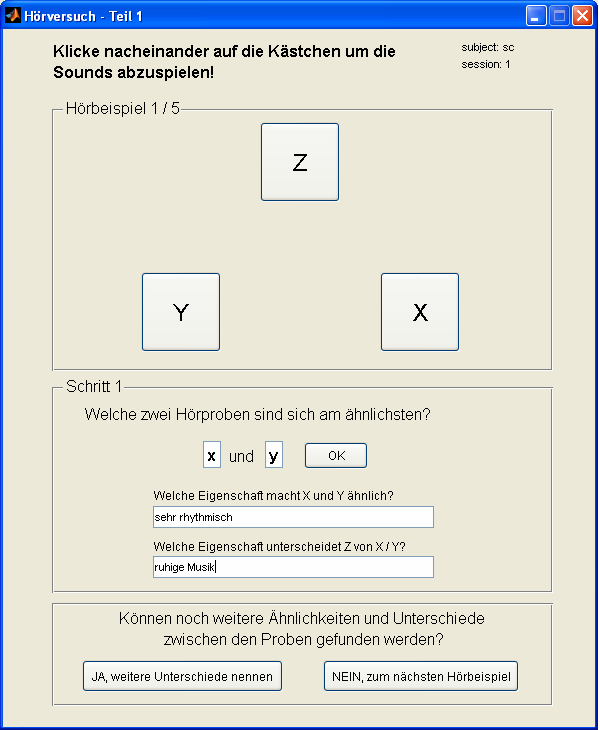
\includegraphics[resolution=150]{rgt_triads_subject.png}
  	\caption[The subject's GUI for the performance of the RGT's first part.]{The subject's GUI for the performance of the RGT's first part, i.e. the triadic comparison.}
  	\label{fig:rgt_triads_subject}
\end{figure}

Figure \ref{fig:rgt_triads_subject} shows the elicitation GUI. To play one of the triad's stimuli the subject has to apply one of the three buttons denoted by \textit{X, Y} and \textit{Z}. The subjects' first task is to decide which two out of the three stimuli appear to be more similar than the third one and then enter the labels of the corresponding two buttons (i.e. X, Y or Z). The inputs must be confirmed by applying the \textit{OK} button. This task is only required to correctly formulate the next two questions which will be presented only, if each stimulus has been played for at least one time. First it is asked in how far the two stimuli which have been previously identified as the most similar ones are alike. Second, it is asked for the difference between these two stimuli and the third one. Please be aware that alternative methods for posing these two questions -- such as asking for a direct negation of the first descriptor -- have been discussed in literature, too. 
\\
After answering these questions, the subject may choose to  either go on reporting further similarites and differences or to continue with the next triad's presentation. Note that the test continues only, if each stimulus has been played for at least one time and all questions have been answered (i.e., inputs have been made to the respective fields). The first part of the procedure ends by displaying an instruction telling the subject to wait for the experimenter.


\paragraph{Break: Editing Constructs}
When the experimenter operates the button labeled \textit{"nur vom Versuchsleiter zu bedienen"} a DW will appear which is labeled as \textit{RGT -- edit constructs} (see Fig. \ref{fig:rgt_edit_constructs}). As with all other experimenter DWs the operating language in this DW is English. Possible modifications of the elicited phrases range from revising construct phrasing, determining assignments to either one of the rating scale's poles, deleting entire constructs, making decisions on the scale's polarity, i.e. its orientation when being posed during the rating process, and changing the order in that scales are posed one below the other. After editing, the experimenter may press the "resume" button in order to start the procedure's second part, i.e. the rating procedure.

\begin{figure}[h]\centering
	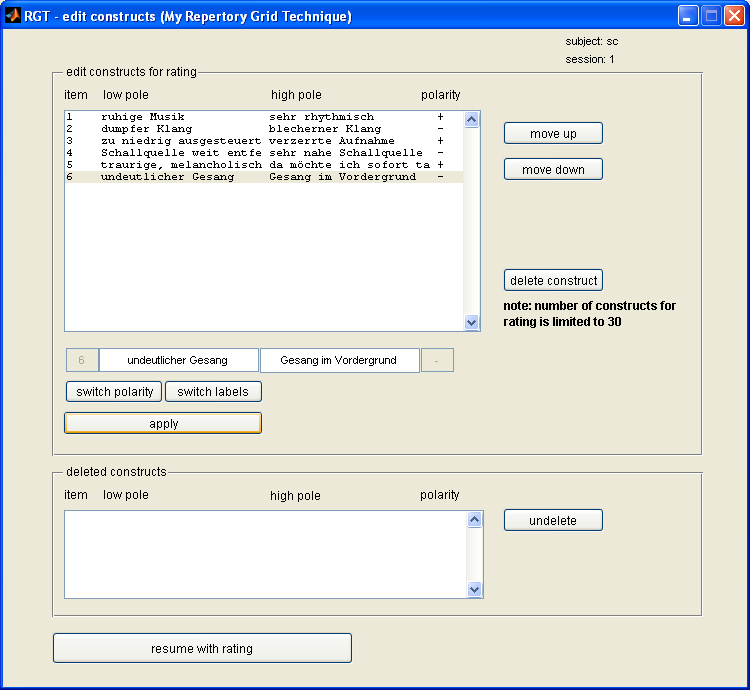
\includegraphics[resolution=150]{rgt_edit_constructs.png}
  	\caption[DW \textit{RGT -- edit constructs (...)}]{The DW \textit{RGT -- edit constructs (...)} offers the possibility to the experimenter for editing the constructs elicited in the first part.}
  	\label{fig:rgt_edit_constructs}
\end{figure}

\minisec{DW \itshape\lqq RGT -- edit constructs (...)\rqq}\medskip
\begin{description}
	\item[subject: ...] (\textit{text}) Displays the ID of the current subject.
	\item[session: ...] (\textit{text}) Displays the key number of the current session.
	\item[edit constructs for rating] (\textit{panel})\hfill
	\begin{description}
		\item[\textrm{\textless}no label\textrm{\textgreater}] (\textit{multi-columned list box}) This list primarily shows the constructs arranged in the order of their elicitation events which is represented by the numbers placed in the first column. After modifications have been made with respect to the order of the list's entries (by using the \textit{move up/move down} buttons, see below) these numbers then represent the order in which the constructs' scales will be posed one below the other during the rating process. The further columns view the poles' verbal descriptors and the scale's polarity, i.e. its orientation when being posed during the rating process. For the latter a \lqq +\rqq\ indicates that the low pole (i.e. the pole belonging to a minimum scale value) will be posed on the left side of the DW and the high pole (i.e. the pole belonging to a maximum scale value) on the right side. The reversed case is indicated by a \lqq -\rqq. Note that at first poles may be not properly defined as the verbal descriptors' assignment either to the scale's minimum or maximum extension has been automatically done straight forward (i.e. the inital pole is always assigned to the low pole and vice versa). A correction then has to be performed manually by using the button \textit{switch labels} which is described below. When all editing work has been completed the list must not contain more than 30 constructs. This restriction is due to the finite display resolution which limits the number of scales to be displayed properly within one window. 
		\item[\textrm{\textless}no label\textrm{\textgreater}] (\textit{output field} 1st col) Displays the number assigned to the selected construct.
		\item[\textrm{\textless}no label\textrm{\textgreater}] (\textit{input/output fields} 2nd \& 3rd col) Spaces for displaying and editing the verbal descriptors of the scale's poles belonging to the selected construct.
		\item[\textrm{\textless}no label\textrm{\textgreater}] (\textit{output field} 4th col) Indicates the polarity of the scale belonging to the selected construct.
		\item[switch polarity] (\textit{button}) Switches polarity of the scale belonging to the selected construct.
		\item[switch labels] (\textit{button}) Switches verbal descriptors of the scale's poles belonging to the selected construct.
		\item[apply] (\textit{button}) Applies changes in the contents of the input/output fields above to the selected construct.
		\item[move up/move down] (\textit{button}) Shifts the selected construct to a proximate list position above/below.
		\item[delete construct] (\textit{button}) Deletes a selected construct which then is shifted to the list below.
	\end{description}
	\item[deleted constructs] (\textit{panel})\hfill
	\begin{description}
		\item[\textrm{\textless}no label\textrm{\textgreater}] (\textit{multi-columned list box}) This list views all constructs that have been deleted from the list above. The idea behind this is to prevent the experimenter from losing a construct by faulty operation, as the items contained in this list can be reassigned to the list above by using the button \textit{undelete} which is described below.
		\item[undelete] (\textit{button}) Reassigns the selected construct to the list above.
	\end{description}
	\item[resume with rating] (\textit{button}) Resumption of the current test section by initiating the RGT's second part, i.e. the rating process. Note: make sure that all editing work has been completed before applying this button, as there will be no possibility to return to this DW afterwards.
\end{description}


\paragraph{Part II: Rating Procedure}
The rating part is introduced by displaying experimenter-defined instructions. After operating the  \textit{weiter}-button the rating procedure begins. 

The respective GUI is shown in figure~\ref{fig:rgt_rating_subject}. The playback of the respective stimulus starts automatically at the beginning of each trial. To allow for a short delay the experimenter can specify a suitable time period (see sec.~\ref{rgt_setup}). Rating is allowed from the beginning of a trial (even during the playback) either on discrete scales which are realized by radio buttons. Progression to the next stimulus is possible if the whole set of -- at most 30 -- constructs has been rated. This restriction is due to the finite display resolution preventing displaying a greater number of scales together with their poles' labels within one window.

\begin{figure}[h]\centering
	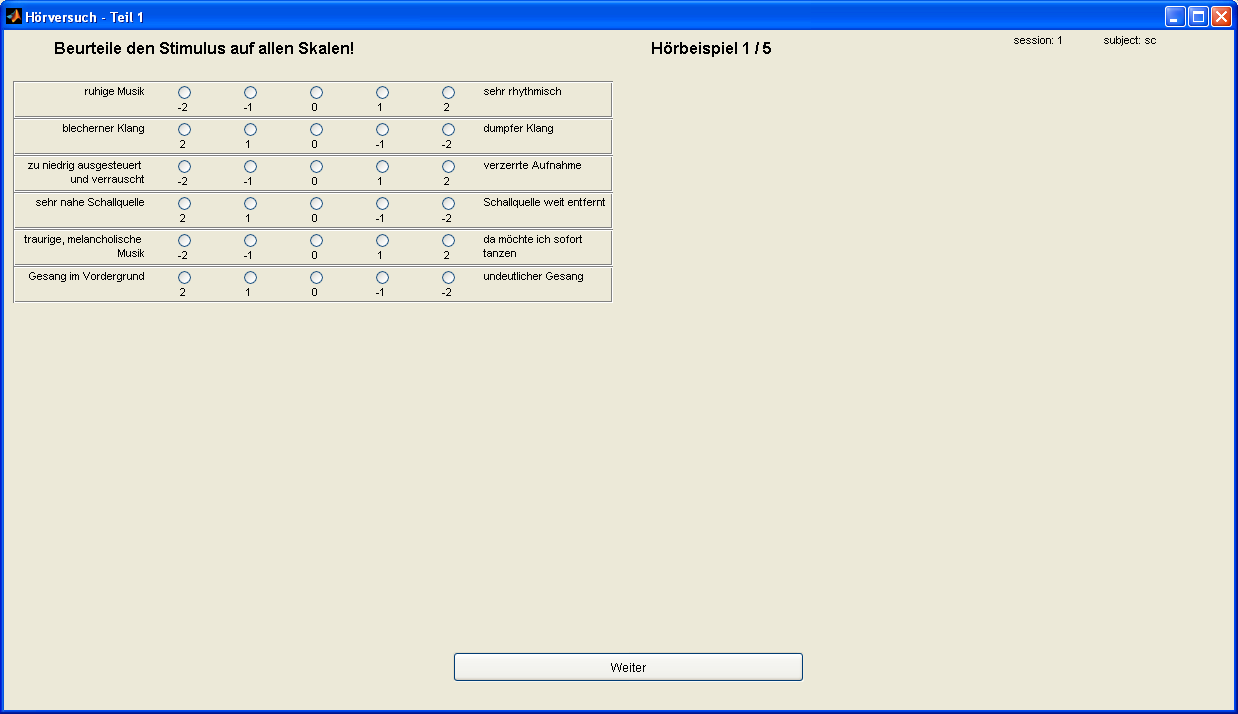
\includegraphics[width = \textwidth]{rgt_rating_subject.png}
 		\caption[The subject's GUI for the performance of the RGT's second part.]{The subject's GUI for the performance of the RGT's second part, i.e. the rating of the elements on the constructs which have been elicited and edited before.}
  	\label{fig:rgt_rating_subject}
\end{figure}


\subsection{Setting up Properties}\label{rgt_setup}
Settings of the procedure's properties have to be determined on the DW \textit{RGT -- main settings (...)} which can be accessed as explained in section \ref{procedure_parameters}. The basis for the whole procedure is formed by the definition of elements which is done in the respective DW accessible by the button \textit{element pool}. Thereby, a set of stimuli from the stimulus pool can be selected and assigned to element key numbers, gathered in the \textit{element pool}. Further settings are structured by the procedure's two parts and hence adjustable in two distinct panels. 

If elements have been defined, the generation of the triads can be performed on the panel \textit{Part I: construct elicitation} by applying the button \textit{edit triads} which then opens a DW that allows either to manually assign elements to the triads' key numbers or to let the program automatically generate a complete variation of (at most 15) elements over triads which then may be edited manually. 
\\
After defining the triads the order of their presentation has to be determined. This can be done in two different ways: On the one hand one may choose to play all triads in a random order, whereas on the other hand one may select certain triads which can either be played in a determined sequence or in random succession. When choosing the second approach one has to apply the regarding \textit{edit} button to reach the respective DW labeled as \textit{RGT -- triad sequence setup (...)} which is described in more detail below. A further property that can be set is the maximum possible number of constructs the experimenter wants to be drawn during one triadic comparison (cp. sec~\ref{rgt_run}). Moreover, two instructions may be entered. The first one will be displayed in the beginning of the procedure's first part whereas the second one should consist only of a short phrase which will be placed on top of the triadic comparison panel.

Setting the properties of the second part (rating) has to be performed on the panel \textit{Part II: rating procedure}. By applying the button \textit{edit scales} one gets to the DW \textit{RGT -- edit scale format} which is described below and allows adjusting the scales' format settings such as the number of categories, the categories' numerical representatives, category labels if required. 
\\
Further parameters of the rating process refer to the order of the elements' presentation and will be adjusted in a manner that is completely analogous to the approach already described above in the triads' context. Moreover, the time period between the subject's operation of the \textit{weiter}-button and the presentation of the next element can be fixed. Finally, two different instructions may be entered. Again, two instructions may be entered. The first one will be displayed in the beginning of the procedure's second part whereas the second one should consist only of a short phrase which will be placed on top of the rating panel.

\begin{figure}[h]\centering
	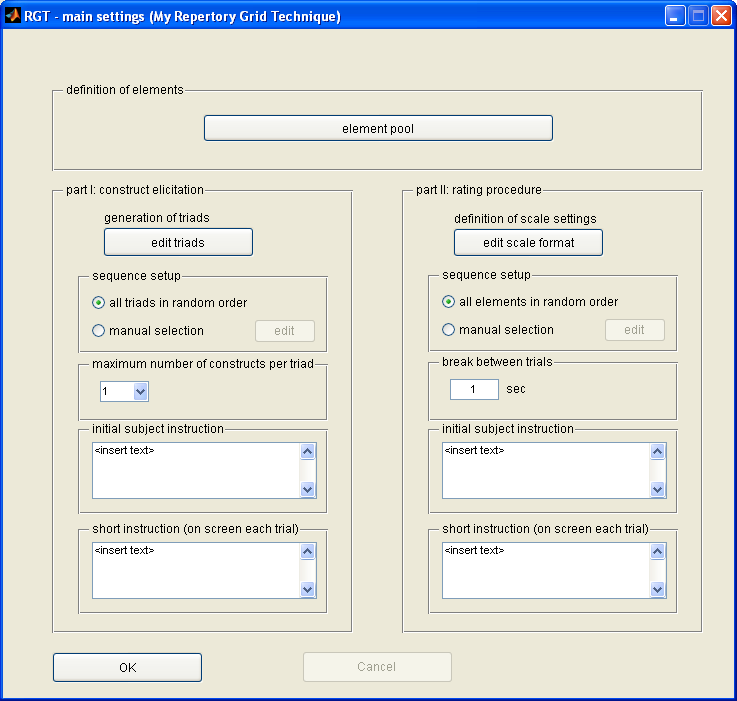
\includegraphics[resolution=150]{rgt_main_settings.png}
  	\caption{DW \textit{RGT -- main settings (...)}}
  	\label{fig:rgt_main_settings}
\end{figure}

\pagebreak[4]\minisec{DW \itshape\lqq RGT -- main settings (...)\rqq}\medskip
\begin{description}
	\item[definition of elements] (\textit{panel})\hfill
	\begin{description}
		\item[element pool] (\textit{button}) Opens a DW for definition of the elements by assigning stimuli from the stimulus pool to the elements' key numbers which are listed in the \textit{element pool}. 
	\end{description}\pagebreak[2]
	\item[Part I: construct elicitation] (\textit{panel})\hfill
	\begin{description}
		\item[edit triads] (\textit{button}) Opens a DW for generation of triads. The latter can either be performed manually by assigning three elements respectively to each triad's key number or by automatically generating a complete variation. In the latter case it is possible to permute 15 elements at most yielding a list of 455 triads.
		\item[sequence setup] (\textit{sub-panel}) \hfill
		\begin{description}
			\item[all triads in random order] (\textit{radio button}) If selected, the complete list of triads generated before will be presented to each subject in a random order.
			\item[manual selection] (\textit{radio button}) If selected, only a selection of triads, i.e. a subset of the triad list, will be presented to each subject with sequences either being randomly generated or predefined (see button \textit{edit} below).
			\item[edit] (\textit{button}) Opens a DW labeled as \textit{RGT -- triad sequence setup (...)} and described below, for selection of subsets of triads and determination of their orders of presentation.
		\end{description}
		\item[maximum number of constructs per triad] (\textit{sub-panel})\hfill
		\begin{description}
			\item[\textrm{\textless}no label\textrm{\textgreater}] (\textit{drop-down list}) Here you can choose the maximum number of constructs that may result from one triad comparison. Subjects will then have the opportunity to report on a respective quantity of attributes if they intend to. 
		\end{description}
		\item[initial subject instruction] (\textit{sub-panel})\hfill
		\begin{description}
			\item[\textrm{\textless}no label\textrm{\textgreater}] (\textit{multi-lined input field}) Space for entering terms of instructions that will be displayed on the subject's \textit{basic screen} (see sec.~\ref{testrun}) before the test section (i.e. the first part of the RGT) is started. The input will be treated as a string.
		\end{description}
		\item[short instruction (on screen each trial)] (\textit{sub-panel})\hfill
		\begin{description}
			\item[\textrm{\textless}no label\textrm{\textgreater}] (\textit{multi-lined input field}) Space for entering a short term of instruction that will be displayed on top of the subject's user interface in each trial. The input will be treated as a string.
		\end{description}
	\end{description}
	
	\item[Part II: rating procedure] (\textit{panel})\hfill
	\begin{description}
		\item[edit scales] (\textit{button}) Opens a DW labeled as \textit{RGT -- edit scale settings (...)} and described below, for editing the format settings of the rating scales.
		\item[sequence setup] (\textit{sub-panel}) \hfill
		\begin{description}
			\item[all elements in random order] (\textit{radio button}) If selected, all defined elements will be presented to each subject in a random order.
			\item[manual selection] (\textit{radio button}) If selected, only a selection of elements, i.e. a subset of the element pool, will be presented to each subject with sequences either being randomly generated or predefined (see button \textit{edit} below).
			\item[edit] (\textit{button}) Opens a DW labeled as \textit{RGT -- element sequence setup (...)} and described below, for selection of subsets of elements and determination of their orders of presentation during the rating process.
		\end{description}
		\item[break between trials] (\textit{sub-panel})\hfill
		\begin{description}
			\item[\textrm{\textless}no label\textrm{\textgreater}] (\textit{input field}) Space for entering the time period in seconds that lies between the subject's activation of the \textit{weiter} button after finishing rating on the current stimulus (i.e. element) and the initiation of presentation of its successor. The input will be treated as a double value.
		\end{description}
		\item[initial subject instruction] (\textit{sub-panel})\hfill
		\begin{description}
			\item[\textrm{\textless}no label\textrm{\textgreater}] (\textit{multi-lined input field}) Space for entering terms of instructions that will be displayed on the subject's \textit{basic screen} (see sec.~\ref{testrun}) before the second part of the RGT (i.e. the rating of the elements) is started. The input will be treated as a string.
		\end{description}
		\item[short instruction (on screen each trial)] (\textit{sub-panel})\hfill
		\begin{description}
			\item[\textrm{\textless}no label\textrm{\textgreater}] (\textit{multi-lined input field}) Space for entering a short term of instruction that will be displayed on top of the subject's user interface in each trial. The input will be treated as a string.
		\end{description}
	\end{description}
\end{description}

\begin{figure}[h]\centering
	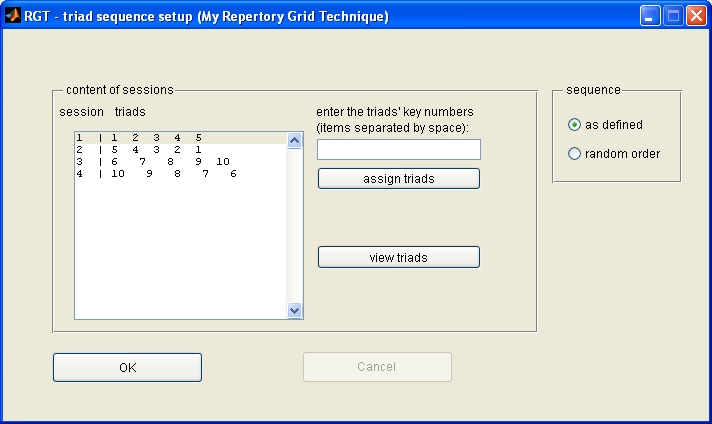
\includegraphics[resolution=150]{rgt_sequence_setup.png}
  	\caption{DW \textit{RGT -- triad/element sequence setup (...)}}
  	\label{fig:rgt_sequence_setup}
\end{figure}

The following description of a DW refers to the manual selection and determination of sequences of both triads and elements.

\minisec{DW \itshape\lqq RGT -- triad/element sequence setup (...)\rqq}\medskip
\begin{description}
	\item[contents of sessions] (\textit{panel})\hfill
	\begin{description}
		\item[\textrm{\textless}no label\textrm{\textgreater}] (\textit{multi-columned list box}) Shows all sessions that have been defined earlier (see sec.~\ref{sessions_setup}) and their belonging subsets of selected triads/elements.
		\item[separate items by space] (\textit{input field}) Space for entering the key numbers of the triads/elements one wants to be presented during the regarding session. Items have to be separated by space.
		\item[assign triads/elements] (\textit{button}) Assigns the content of the previously described input field to the session currently selected. Preexisting content will be overwritten.
		\item[view triads/elements] (\textit{button}) Shows the list of triads/elements defined earlier (see button \textit{edit triads/element pool} above).
	\end{description}
	\item[sequence] (\textit{panel})\hfill
	\begin{description}
		\item[as defined] (\textit{radio button}) If selected, the sequence of presentation will be the same as the order of the items entered to the field previously described.
		\item[random order] (\textit{radio button}) If selected, the sequence of presentation will be randomly generated before each run.
	\end{description}
\end{description}

\begin{figure}[h]\centering
	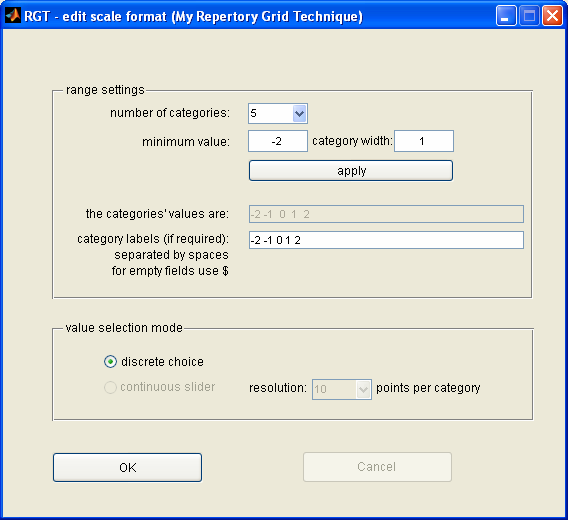
\includegraphics[resolution=150]{rgt_edit_scale_format.png}
  	\caption{DW \textit{RGT -- edit scale format (...)}}
    \label{fig:rgt_edit_scale_format}
\end{figure}

\minisec{DW \itshape\lqq RGT -- edit scale format (...)\rqq}\medskip
\begin{description}
	\item[range settings] (\textit{panel})\hfill
	\begin{description}
		\item[number of categories] (\textit{drop-down list}) Here you can choose a number of categories that is inbetween 2 and 11. By default it's set to 5.
		\item[minimum value] (\textit{input field}) Space for entering the minimum value of the scale's range. By default it's set to -2.
		\item[category width] (\textit{input field}) Space for entering the category width. By default it's set to 1. 
		\item[apply] (\textit{button}) Calculates the categories' numerical representatives.
		\item[your category values are] (\textit{output field}) Displays the categories' numerical representatives if calculated before by using the \textit{apply} button.
		\item[category labels (if required)] (\textit{input field}) Space for entering the category labels if required. The single inputs will be treated as strings that have to be separated by space and are assigned to the categories in ascending order of their numerical representatives. If you want to skip a category enter a \$-sign.
	\end{description}
	\item[value selection mode] (\textit{panel})\hfill
	\begin{description}
		\item[discrete choice] (\textit{radio button}) If selected, the subject will only be able to choose a point on the scale that belongs to one of the categories' marks. Selection is made by using radio buttons.
		\item[continuous slider] (\textit{radio button}) \textless not available at the program's present state\textgreater
		\item[resolution] (\textit{drop-down list}) \textless not available at the program's present state\textgreater
	\end{description}
\end{description}


\section{Semantic Differential (SD)}\label{sd}
\subsection{The Test Run}\label{sd_run}
The procedure-specific user interface is depicted in figure~\ref{fig:sd_subject}. The playback of the respective stimulus starts automatically at the beginning of each trial. To allow for a short delay the experimenter can specify a suitable time period (see sec.~\ref{sd_setup}). Rating is allowed from the beginning of a trial (even during the playback) either on discrete scales which are realized by radio buttons. Progression to the next stimulus is possible if the whole set of -- at most 30 -- constructs has been rated. This restriction is due to the finite display resolution preventing displaying a greater number of scales together with their poles' labels within one window.

\begin{figure}[h]\centering
	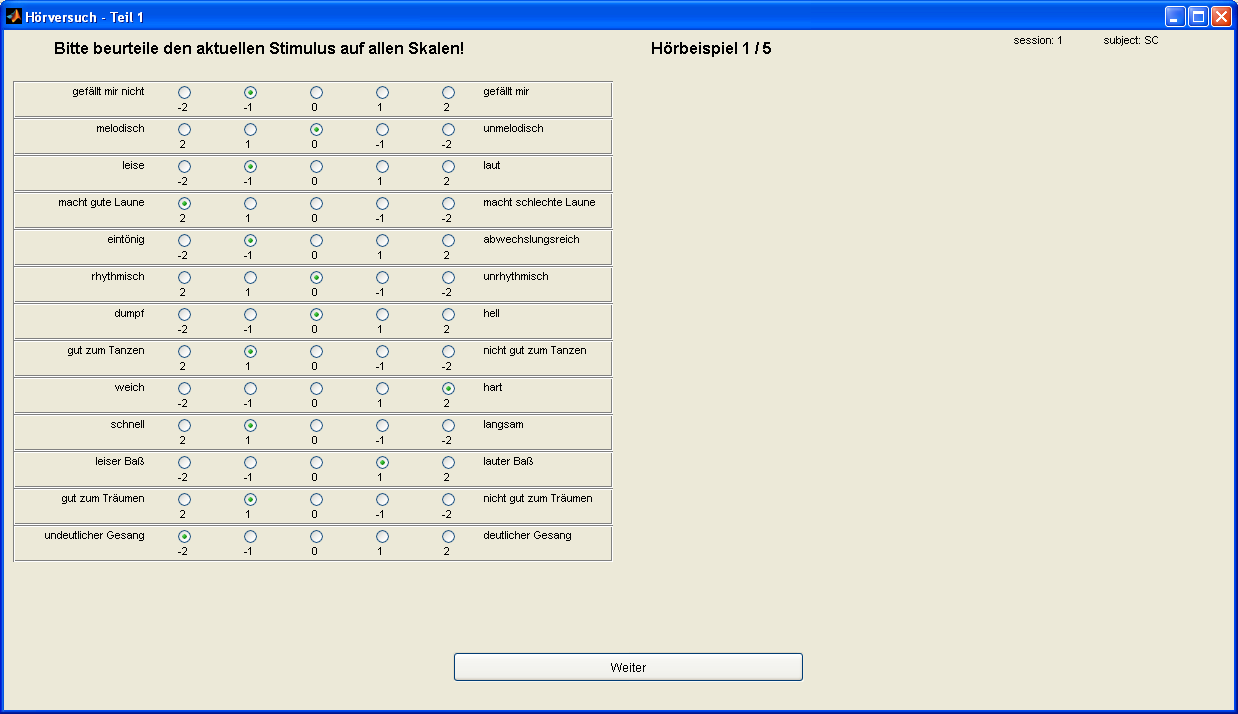
\includegraphics[width = \textwidth]{sd_subject.png}
 	\caption{The subject's GUI for performing the SD test.}
  \label{fig:sd_subject}
\end{figure}

\subsection{Setting up Properties}\label{sd_setup}
The procedure's settings may be edited in the DW \textit{SD -- main settings (...)} which is depicted in figure~\ref{fig:sd_main_settings} and can be accessed as explained in subsection \ref{procedure_parameters}. Its control elements will be described below. In the beginning, objects (i.e. stimuli) to be rated have to be defined using the DW \textit{SD -- object pool (...)} (see fig.~\ref{fig:sd_object_pool} on p.~\pageref{fig:sd_object_pool})\label{textref:object_pool} accessible by the button \textit{object pool}. Thereby, a set of stimuli from the stimulus pool can be selected and assigned to object key numbers, gathered in the \textit{object pool}. By applying the button \textit{edit scales} the DW \textit{SD -- edit scales} (see fig.~\ref{fig:sd_edit_scales} on p.~\pageref{fig:sd_edit_scales}) is opened. The DW allows adjusting the scales' format settings such as the number of categories, the categories' numerical representatives, and category labels if required. Moreover, verbal descriptors of the scales' endpoints can be defined. Further settings refer to the order of the objects' presentation and can be adjusted in the panel \textit{sequence setup}. Here, one can choose the generation of a random sequence or define a sequence manually by applying the button \textit{edit} whic opens a DW \textit{SD -- object sequence setup (...)} (see fig.~\ref{fig:sd_object_sequence_setup} on p.~\pageref{fig:sd_object_sequence_setup}). Moreover, the time period between the subject's actuation of the \textit{weiter}-button and the presentation of the next object can be fixed. Finally, two instruction texts can be defined. The first one will be displayed at the beginning of the procedure, the second one, which should consist of a short phrase only, which will be shown on the top of the subject's user interface in each trial.

\begin{figure}[h]\centering
	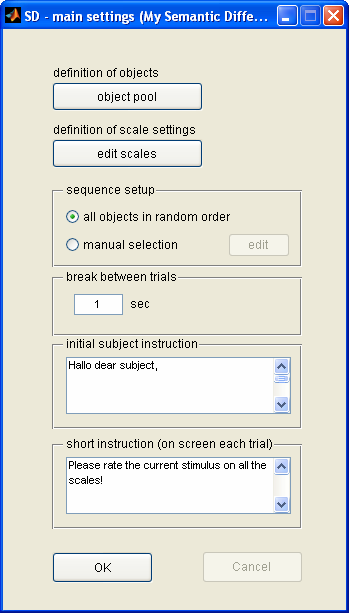
\includegraphics[resolution=150]{sd_main_settings.png}
  	\caption{DW \textit{SD -- main settings (...)}}
    \label{fig:sd_main_settings}
\end{figure}

\minisec{DW \itshape\lqq SD -- main settings (...)\rqq}\medskip
\begin{description}
	\item[object pool] (\textit{button}) Opens a DW for definition of the objects by assigning stimuli from the stimulus pool to the objects' key numbers which are listed in the \textit{object pool}. 
	\item[edit scales] (\textit{button}) Opens a DW labeled as \textit{SD -- edit scales (...)} and described below, for editing the formal settings of the rating scales and defining the endpoints' verbal descriptors. 
	\item[sequence setup] (\textit{panel})\hfill
	\begin{description}
		\item[all objects in random order] (\textit{radio button}) If selected, all objects will be presented to each subject in a random order.
		\item[manual selection] (\textit{radio button}) If selected, only a selection of objects, i.e. a subset of the object pool, will be presented to each subject with sequences either being randomly generated or predefined.
		\item[edit] (\textit{button}) Opens a DW labeled as \textit{SD -- object sequence setup (...)} and described below, for selection of subsets of objects and determination of their orders of presentation.
	\end{description}
	\item[break between trials] (\textit{panel})\hfill
	\begin{description}
	  \item[\textrm{\textless}no label\textrm{\textgreater}] (\textit{input field}) Space for entering the time period in [sec] that lies between the subject's actuation of the \textit{weiter} button after finishing rating on the current stimulus (i.e. object) and the initiation of its successor's presentation. The input will be treated as a double value.
  \end{description}
  \item[initial subject instruction] (\textit{panel})\hfill
	\begin{description}
		\item[\textrm{\textless}no label\textrm{\textgreater}] (\textit{multi-lined input field}) Space for entering terms of instructions that will be displayed on the subject's \textit{basic screen} (see sec.~\ref{testrun}) before the test section is started.
	\end{description}
	\item[short instruction (on screen each trial)] (\textit{panel})\hfill
		\begin{description}
			\item[\textrm{\textless}no label\textrm{\textgreater}] (\textit{multi-lined input field}) Space for entering a short term of instruction that will be displayed on top of the subject's user interface in each trial.
		\end{description}
\end{description}

\begin{figure}[h]\centering
	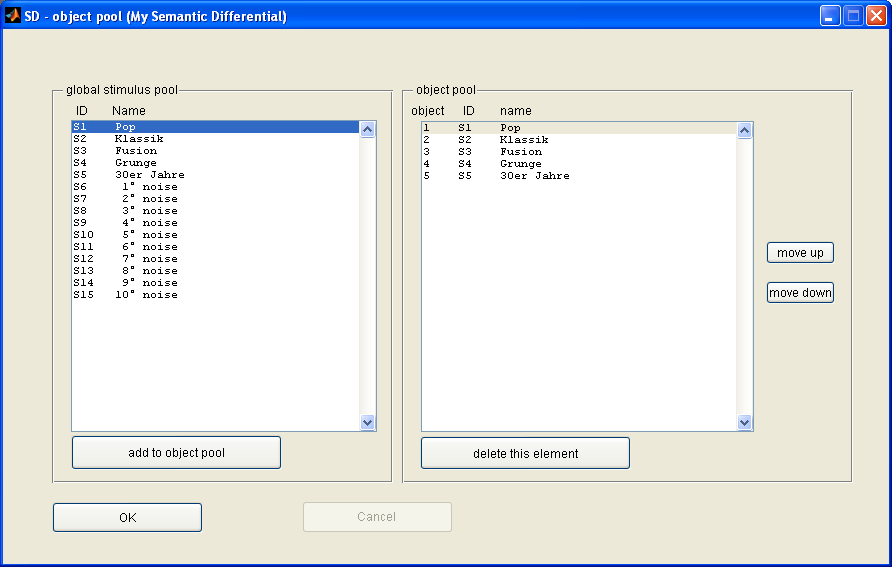
\includegraphics[resolution=150]{sd_object_pool.png}
  	\caption{DW \textit{SD -- object pool (...)} (see text on p.~\pageref{textref:object_pool})}
    \label{fig:sd_object_pool}
\end{figure}

\begin{figure}[h]\centering
	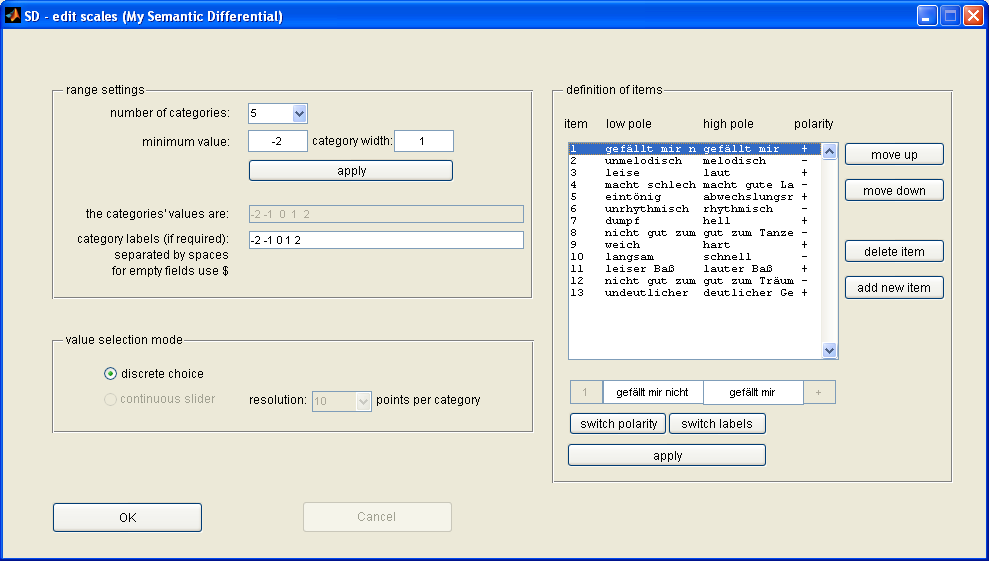
\includegraphics[width=\textwidth]{sd_edit_scales.png}
  	\caption{DW \textit{SD -- edit scales (...)}}
    \label{fig:sd_edit_scales}
\end{figure}

\pagebreak[4]\minisec{DW \itshape\lqq SD -- edit scales (...)\rqq}\medskip
\begin{description}
	\item[range settings] (\textit{panel})\hfill
	\begin{description}
		\item[number of categories] (\textit{drop-down list}) Here you can choose a number of categories that is in between 2 and 11. By default it's set to 5.
		\item[minimum value] (\textit{input field}) Space for entering the minimum value of the scale's range. By default it's is set to -2.
		\item[category width] (\textit{input field}) Space for entering the category width. By default it's set to 1. 
		\item[apply] (\textit{button}) Calculates the categories' numerical representatives.
		\item[the categories' values are] (\textit{output field}) Displays the categories' numerical representatives if calculated before by using the \textit{apply} button.
		\item[category labels (if required)] (\textit{input field}) Space for entering the category labels if required. The single inputs will be treated as strings that have to be separated by space and are assigned to the categories in ascending order of their numerical representatives. If you want to skip a category enter a \$-sign.
	\end{description}
	\item[value selection mode] (\textit{panel})\hfill
	\begin{description}
		\item[discrete choice] (\textit{radio button}) If selected, the subject will only be able to choose a point on the scale that belongs to one of the categories' marks. Selection is made by using radio buttons.
		\item[continuous slider] (\textit{radio button}) \textless not available at the program's present state\textgreater
		\item[resolution] (\textit{drop-down list})\textless not available at the program's present state\textgreater
	\end{description}
	\item[item definition] (\textit{panel})\hfill
	\begin{description}
		\item[\textrm{\textless}no label\textrm{\textgreater}] (\textit{multi-columned list box}) This list shows the scales' endpoint descriptors representing the \textit{items} under test, i.e. the attributes underlying the affective or perceptual measurement. During the test run the items and their belonging scales will be placed on the screen in the same order as they are created in the list. The further columns view the poles' verbal descriptors and the scale's polarity, i.e. its orientation when being posed during the test run. For the latter a \lqq +\rqq\ indicates that the low pole (i.e. the pole belonging to a minimum category value) will be posed on the left side of the DW and the high pole (i.e. the pole belonging to a maximum category value) on the right side. The reversed case is indicated by a \lqq -\rqq. The list may not contain more than 30 items. This restriction is due to the finite display resolution as a greater number would lead to problems with viewing all scales and their labels within one common window. 
		\item[\textrm{\textless}no label\textrm{\textgreater}] (\textit{output field} 1st col) Displays the selected item's number which also represents its position within the order of presentation during the test run.
		\item[\textrm{\textless}no label\textrm{\textgreater}] (\textit{input/output fields} 2nd \& 3rd col) Spaces for displaying and editing the verbal descriptors of the scale's poles belonging to the selected item.
		\item[\textrm{\textless}no label\textrm{\textgreater}] (\textit{output field} 4th col) Indicates the polarity of the scale belonging to the selected item.
		\item[switch polarity] (\textit{button}) Switches polarity of the scale belonging to the selected item.
		\item[switch labels] (\textit{button}) Switches verbal descriptors of the scale's poles belonging to the selected item.
		\item[apply] (\textit{button}) Applies changes on the contents of the input/output fields described above to the selected item.
		\item[move up/move down] (\textit{button}) Shifts the selected item to a proximate list position above/below.
		\item[delete item] (\textit{button}) Deletes a selected item.
		\item[add new item] (\textit{button}) Adds a new item to the list after its last position. 
	\end{description}
\end{description}

\begin{figure}[h]\centering
	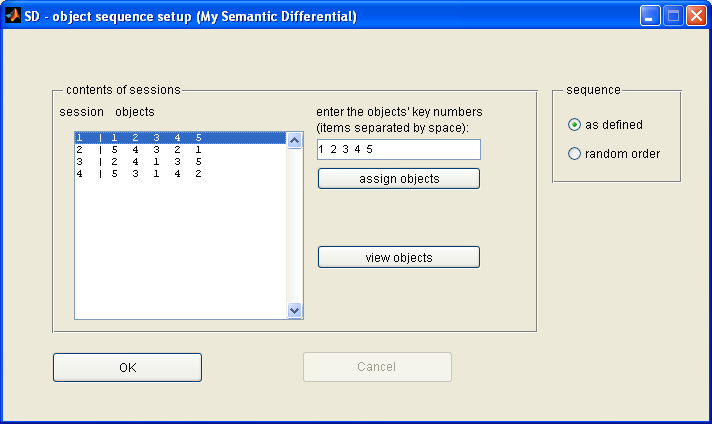
\includegraphics[resolution=150]{sd_object_sequence_setup.png}
  	\caption{DW \textit{SD -- object sequence setup (...)}}
    \label{fig:sd_object_sequence_setup}
\end{figure}

\minisec{DW \itshape\lqq SD -- object sequence setup (...)\rqq}\medskip
\begin{description}
	\item[contents of sessions] (\textit{panel})\hfill
	\begin{description}
		\item[\textrm{\textless}no label\textrm{\textgreater}] (\textit{multi-columned list box}) Shows all sessions that have been defined earlier (cp. sec.~\ref{sessions_setup}) and their belonging subsets of selected objects.
		\item[enter the objects' key numbers (...)] (\textit{input field}) Space for entering the key numbers of the objects one wants to be presented during the regarding session. Items have to be separated by space.
		\item[assign objects] (\textit{button}) Assigns the content of the previously described input field to the session currently selected. Preexisting content will be overwritten.
		\item[view objects] (\textit{button}) Shows the list of objects defined earlier.
	\end{description}
	\item[sequence] (\textit{panel})\hfill
	\begin{description}
		\item[as defined] (\textit{radio button}) If selected, the sequence of presentation will be the same as the order of the items entered to the field previously described.
		\item[random order] (\textit{radio button}) If selected, the sequence of presentation will be randomly generated before each run.
	\end{description}
\end{description}


\section{ABX Detection Test (ABX)}\label{abx}

The ABX test (see also sec. \ref{sec:testprocedures}) is a 2AFC double blind detection test allowing to assess the detectability of very subtle differences between two stimuli while controlling type-1 error level and test power for a pre-defined effect size (the remaining detection rate). For further information about the ABX procedure and its parameters see \citealp{burstein:1988}, \citealp{clark:1991},\citealp{leventhal:1986}. 

\subsection{The Test Run}\label{abx_run}

The subject's GUI while performing an ABX test is divided into two parts (see fig.~\ref{fig:abx_subject}): In  the upper one, the subject can start/stop the audition of three stimuli whereas in the lower section the subject may answer the question, which of the stimuli A or B equals the reference X. 
\\
When hitting the buttons A or B or X, the respective stimulus will be started from the beginning. In the lower section of the test subjects's GUI (below an optional short question/instruction definable in the DW \textit{ABX -- edit main settings}) you will find two answer buttons A and B. After hitting one of them, the \textit{weiter}-button will be activated, allowing the subject to go on to the next trial. \whisper\  registers only the last decision of a subject on a trial, so it is possible to change the given answer multiple times before going to the next trial. 

\begin{figure}[h]\centering
	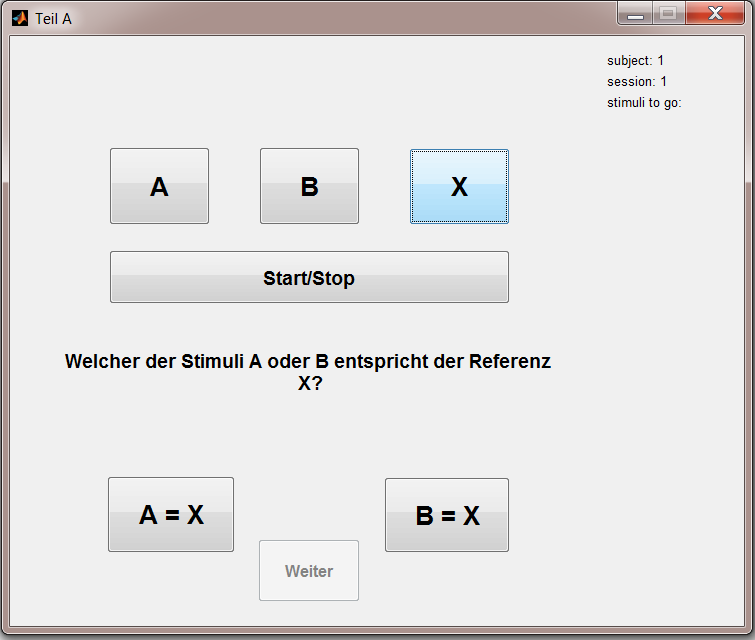
\includegraphics[width = \textwidth]{abx_subject.png}
	\caption{The subject's GUI during an A/B/X trial.}
	\label{fig:abx_subject}
\end{figure}

\subsection{Setting up Properties}\label{abx_setup}
To perform the ABX test, the investigator has to:
\begin{enumerate}
	\item Define the number of trials n (at best using a calculation based on pre-defined type I and II error levels and effect size which can be done directly in the DW {\itshape\lqq ABX -- edit main settings (...)\rqq}),
	\item Assign the stimuli to A and B, and 
	\item Define the instruction texts for the subjects.
\end{enumerate}


\begin{figure}[h]\centering
	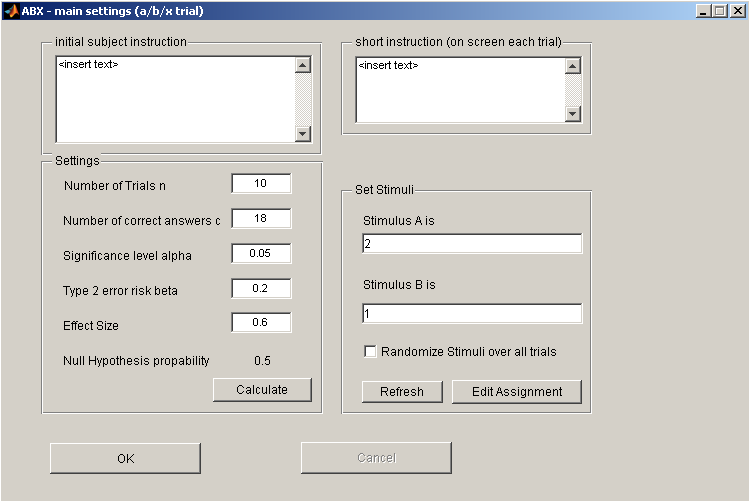
\includegraphics[width = \textwidth]{abx_main_settings.png}
 	\caption{ABX Trial Main Settings}
  \label{fig:abx_editmain}
\end{figure}

\minisec{DW \itshape\lqq ABX -- edit main settings (...)\rqq}\medskip
\begin{description}
	\item[initial subject instruction] (\textit{input field})\hfill
	\begin{description}
		  \item The text shown to the subject before the ABX test starts
	\end{description}
	\item[short instruction] (\textit{input field})\hfill
	\begin{description}
		  \item The text shown in every trial on the subject's GUI
	\end{description}
	\item[number of trials n] (\textit{input field})\hfill
	\begin{description}
		  \item Number of repetitions, Value that defines the length of the ABX test
	\end{description}
	\item[number of correct answers c] (\textit{input field})\hfill
	\begin{description}
		\item Setting this value and fill out the "number of trials"-field and press the "Calculate"-button will result in the corresponding "Significance Level"
	\end{description}
\end{description}
\newpage
\begin{description}
	\item[Significance level alpha] (\textit{input field})\hfill
	\begin{description}
		  \item setting this value as well as the "Type II error risk" and the "Effect size" while leaving empty the "Number of trials"-field and the "Number of correct answers"-field will -- on operating the "Calculate"-button -- result in the corresponding entries to be filled in automatically.
	\end{description}
	\item[type 2 error risk beta] (\textit{input field})\hfill
	\begin{description}
		 \item see "Significance level"
	\end{description}
	\item[Effect size] (\textit{input field})\hfill
	\begin{description}
		 \item see "Significance level"
	\end{description}
	\item[Set Stimuli] (\textit{input field})\hfill
	\begin{description}
		 \item by pressing "Edit Assignment" the DW \textit{ABX -- stimulus assignment(...)} (see Fig. \ref{fig:abx_assign} will be opened. Here, one may define, which of the stimuli (as defined in the main menu) shall be compared in the ABX test. By pressing the "Assign to ..."-buttons one may assign certain stimuli to be either stimulus A and B in the test. By hitting the "refresh"-button in the main settings menu, the assigned stimuli will show up in the "Set Stimuli" display, too, for control. \textbf{Note again here}, that while A and B are assigned to be fixed throughout the whole test, the reference X is of course randomly assigned to be either A, or B resp. in each trial. 
	\end{description}
\end{description}

\begin{figure}[h]\centering
	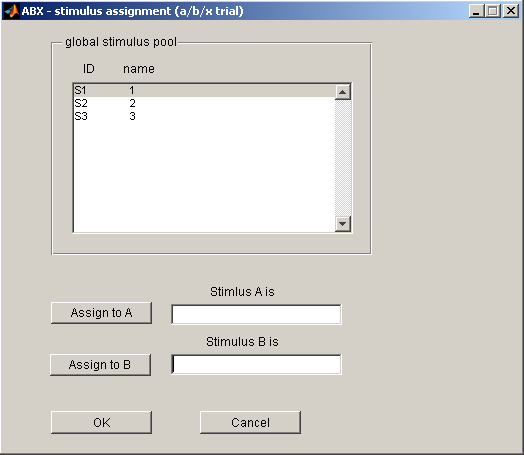
\includegraphics[width = \textwidth]{abx_assign_stimulus.png}
 	\caption{Assigning the stimuli to be judged in the current trial.}
  \label{fig:abx_assign}
\end{figure}
\clearpage

% 7.5 SAQI Martina/Fabian/Alex
\section{Spatial Audio Quality Inventory (SAQI)}\label{saqi}

The Spatial Audio Quality Inventory (SAQI) is intended for a qualitatively differentiated, comparative auditory assessment of real, imagined and simulated acoustic scenes in order to to reveal specific shortcomings of a simulation under test and allow for a directed technical improvement. The SAQI comprises 48 verbal descriptors of perceptual qualities assumed to be of practical relevance when comparing virtual environments (VAEs) to real or imagined references or amongst each other. It was generated by a Focus Group of 20 German experts for virtual acoustics. Five additional experts helped verifying the unambiguity of all descriptors and the related explanations. Moreover, an English translation was generated and verified by seven bilingual experts. Rationale and methodology pursued in constructing the English (SAQI-EN) and the German (SAQI-GER) vocabulary are described in more detail in \cite{lindau:2014a} and \cite{lindau:2014b}. 

The SAQI vocabulary in its entirety (including perceptual descriptors, circumscriptions, scale end label, and - if given - illustrative sound examples) is intended to enable experts in the field to train any laymen to use it for assessments of VAEs. An extensive Test Manual is freely available for download (\cite{lindau:2015}). It is strongly recommended that you read it, in order to better understand the following descriptions of the SAQI test in \whisper. Further, there is a SAQI project website at http://www.ak.tu-berlin.de/saqi.

% 7.5.1 The test run 
\subsection{The Test Run}\label{saqi_run}

The SAQI is a rather extensive test instrument, which can be widely customized to the user's specific needs. If one chooses to conduct a complete SAQI test, rating a singular perceptual difference quality will involve presenting five concurrent GUIs (Graphical User Interfaces) to the listener: 
\begin{enumerate}
	\item quality name and description
	\item rating scale
	\item assignment of modifications (2 GUIs)
	\item choice of assessment entities
\end{enumerate}

Whether this comprehensive way of testing will be actually required will of course depend on the researcher's aims. Whereas only the second GUI will be mandatory (quality name and rating scale) the other four may be optionally used in a test. As an example, in case of more exploratory research questions one might decide to collect as much information as possible, whereas for a more confirmatory study, the SAQI test may be reduced to cover only specific aspects. Hence, the user may conveniently chose from the test settings which assessments shall be conducted (i.e. which GUIs will be shown to the user) in a test run. In the following section it will be shown how a (complete) SAQI evolves from the view of the test subject. In section ~\ref{saqi_setup} it will be explained, how a SAQI test may be parameterized by the experimenter.
\medbreak
By the time, SAQI tests may be conducted in either English and German language (see below). A French translation is currently in the review phase and should be available by the end of 2015.
\medbreak
% Rating GUI
\textbf{Description GUI} \emph{(Fig.~\ref{fig:saqi_circum})}
\medbreak
This GUI is intended for instructing test subjects to focus on a specific auditory quality to be assessed. For each quality it contains the quality's name and a closer circumscription. \textbf{Note:} As described in the SAQI Test Manual (\cite{lindau:2015}) all subjects should be suitably trained to the full understanding of the SAQI \textbf{beforehand}. Therefore, presenting the qualities circumscriptions here is only thought to work as a short reminder.

% screenshoot saqi_circum
\begin{figure}[!h]\centering
	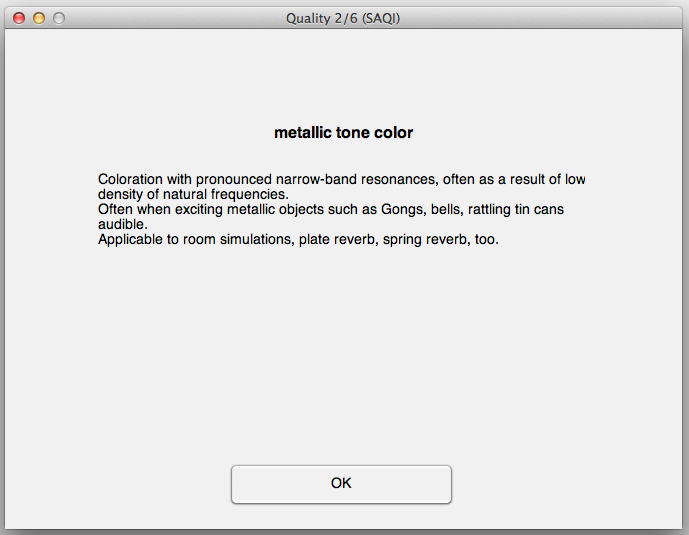
\includegraphics[width = 10cm]{saqi_circumscription.png}
 	\caption{Example of a description GUI presenting a name and circumscription of an auditory quality}
  \label{fig:saqi_circum}
\end{figure}


% Rating GUI
\textbf{Rating GUI} \emph{(Fig.~\ref{fig:saqi_vp2_bip}-\ref{fig:saqi_vp2_multi})}
\medbreak
This GUI is intended for rating the perceived amount of the (described) auditory difference when comparing a test stimulus to a given or imagined reference. For each quality it presents its name, the rating scale and play buttons for playing back the reference and the comparison/test stimuli. The 'OK'-button saves the rating and guides the subject to the next GUI.
\\ 
The design of this GUI will change slightly according to the type of rating scale that belongs to a quality. Most of the qualities in SAQI were found to demand bipolar rating scales represented by sliders, however, two qualities, the 'overall difference' and 'sequence of events', are understood as unipolar. To support a better comparability of ratings, unipolar sliders are displayed with half the length of the bipolar ones.
\\ 
The two qualities 'horizontal direction' and 'vertical direction' are rated using an edit field allowing subjects to directly type in the perceived difference in degree instead of a slider. In addition, there are two radio buttons for indicating the perceived difference in direction (clockwise, or counterclockwise).
\\ 
Finally, one SAQI quality was defined to be dichotomous (difference in 'front-back position'). This descriptor will be rated by using radio buttons: 'not confused' and 'confused'.
\\
If required, up to nine sliders, text fields, or pairs of radio buttons may be presented on one rating screen, this way allowing more efficient testing of multiple stimuli at a time.
\medbreak
\textbf{Note:} For rating the first quality ('overall difference') the user has to listen at least once to the stimuli (i.e. use the play button), otherwise the 'OK'-button won't be enabled. In case the test conditions/stimuli, or the assignment of the test conditions/stimuli to the play \emph{A}, and \emph{B} buttons is randomized, the user has to listen at least once to the stimuli on each rating screen.
\medbreak
\textbf{Note:} By clicking on the text field showing the name of the auditory quality, the description GUI will pop up again.
\\

% screenshoot saqi_vp2_bipolar
\begin{figure}[!h]\centering
	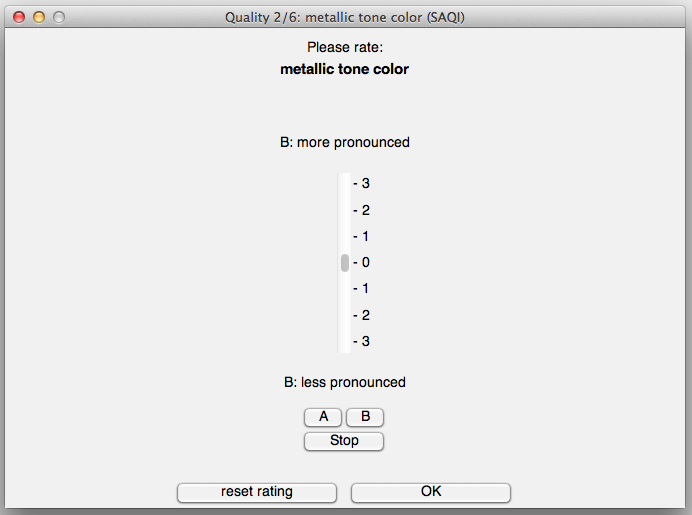
\includegraphics[width = 10cm]{saqi_vp2_bip.png}
 	\caption{Example of a GUI for rating a quality on a bipolar, open-ended rating scale}
  \label{fig:saqi_vp2_bip}
\end{figure}
 
% weitere Skalenversionen (unipolar, dichotom, "degree") 
\begin{figure}[!h]\centering
  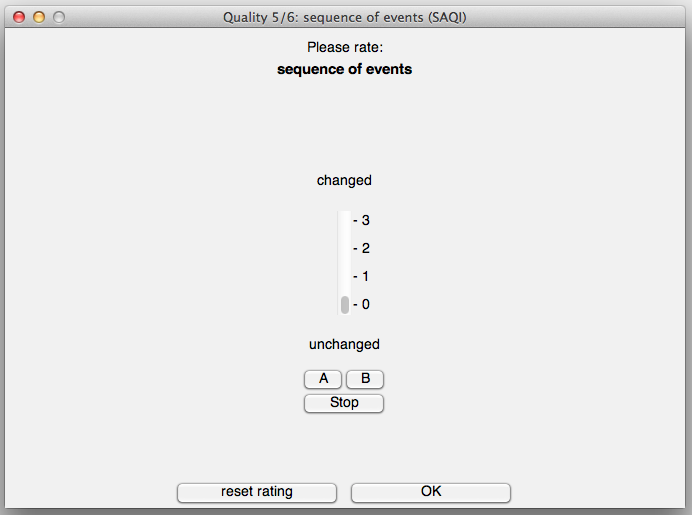
\includegraphics[width = 10cm]{saqi_vp2_uni.png}
  \caption{Example of a GUI for rating a quality using a unipolar, closed/open-ended rating scale}       
  \label{fig:saqi_vp2_uni}
\end{figure}

\begin{figure}[!h]\centering
  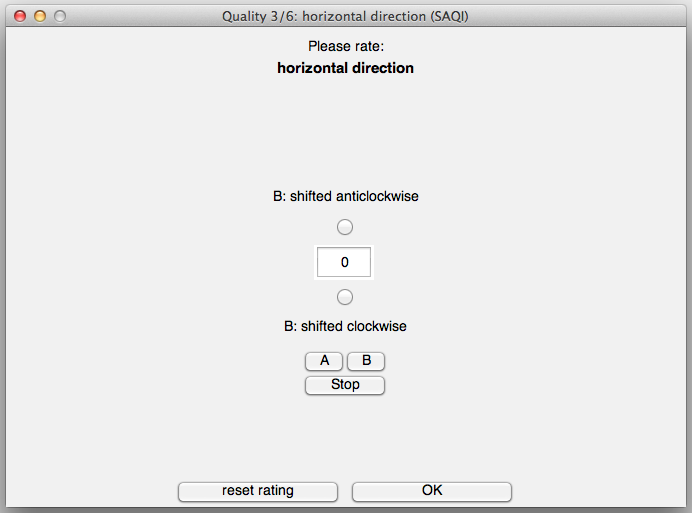
\includegraphics[width = 10cm]{saqi_vp2_deg.png}
  \caption{Example of a GUI for rating a quality using direct bipolar, closed-ended rating}       
  \label{fig:saqi_vp2_deg}
\end{figure}

\begin{figure}[!h]\centering
  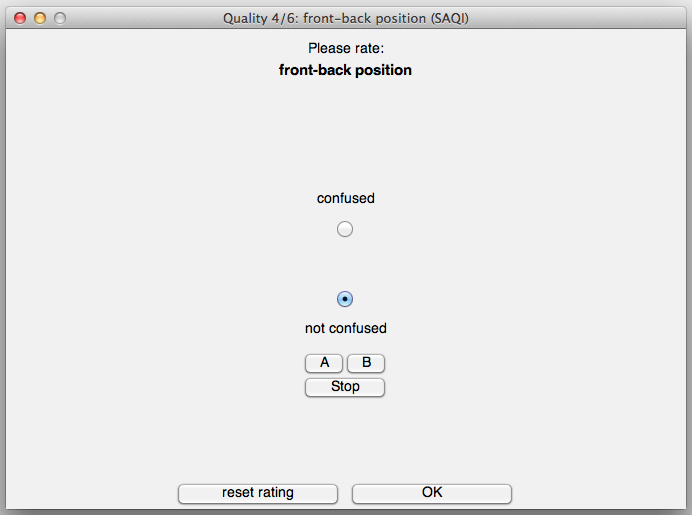
\includegraphics[width = 10cm]{saqi_vp2_dich.png}
  \caption{Example of a GUI for rating a quality using a dichotomous scale}       
  \label{fig:saqi_vp2_dich}
\end{figure}

\begin{figure}[!h]\centering
  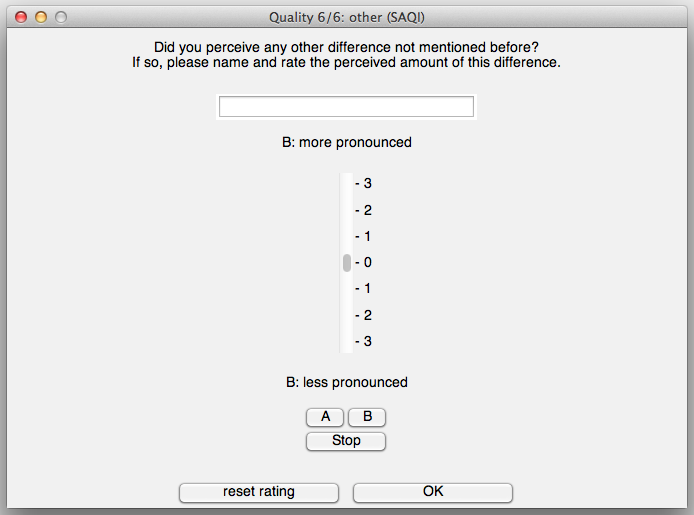
\includegraphics[width = 10cm]{saqi_vp2_other.png}
  \caption{Final GUI asking for formulating and rating any so-far unmentioned differences (SAQI qualifier: \textit{other})}       
  \label{fig:saqi_vp2_other}
\end{figure}

\begin{figure}[!h]\centering
  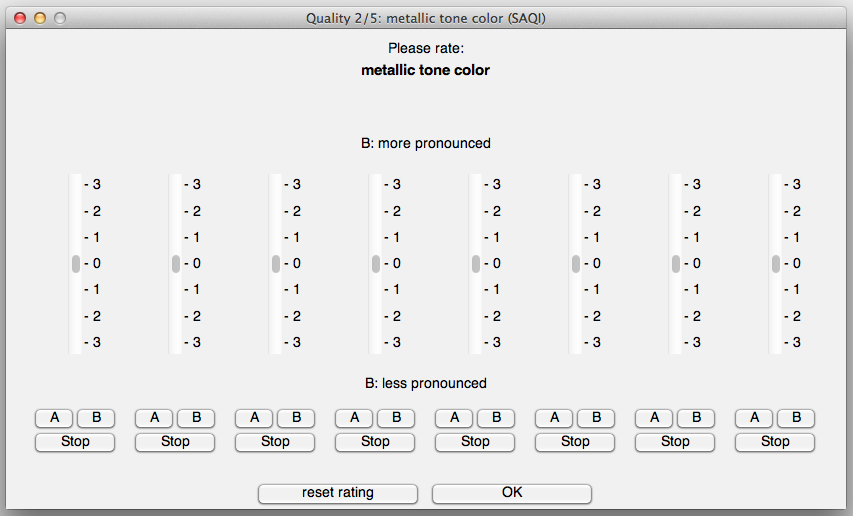
\includegraphics[width = 10cm]{saqi_vp2_multi.png}
  \caption{Example for a rating GUI with eight sliders which allows rating multiple stimuli at a time}       
  \label{fig:saqi_vp2_multi}
\end{figure}

\clearpage
	
% Optional Guis 

\textbf{Optional GUIs} \emph{(Fig.~\ref{fig:saqi_modification_12}-\ref{fig:saqi_entities})}
\medbreak
Since both, a closer description of the perceived qualities by indicating certain modifications, and the assignment of the perceived differences to certain assessment entities is optional, these GUIs will only appear if they were selected before in the test set up. 
\medbreak
\textbf{Note:} Optional GUIs are not available if more then one test condition/stimuli are rated at once (c.f. Fig.~\ref{fig:saqi_vp2_multi}).
\medbreak
The GUIs contain questions referring to the modifications and assessment entities for each single descriptor and will be displayed right after the rating of an perceptual difference in the main GUI. More information about the meaning of modifications and assessment entities can be found in the SAQI Test Manual (\cite{lindau:2015}); related information on the SAQI test setup can be found in sec.~\ref{saqi_setup}.
\\
Please note, that even if the modifications and/or entities are enabled for the test run, they are not going to be displayed if a quality was not rated or was rated with 0 (no difference).

  
% screenshoot modification 1&2
\begin{figure}[!h]\centering
	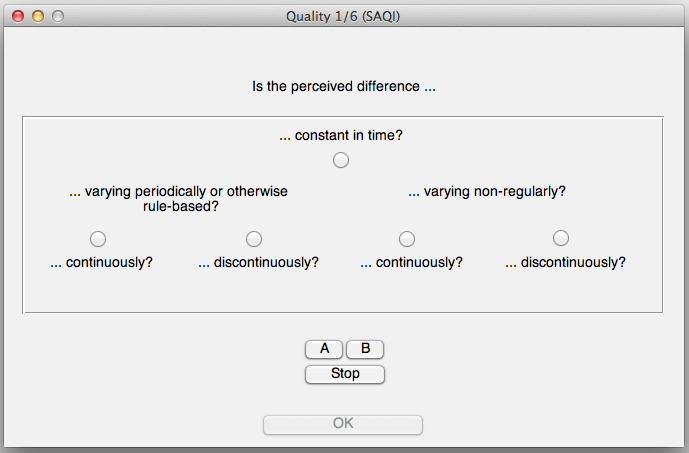
\includegraphics[width = 10cm]{saqi_modification_12.png}
 	\caption{GUI for the rating the temporal variability of perceived differences}
  \label{fig:saqi_modification_12}
\end{figure}
% screenshoot modification 3
\begin{figure}[!h]\centering
	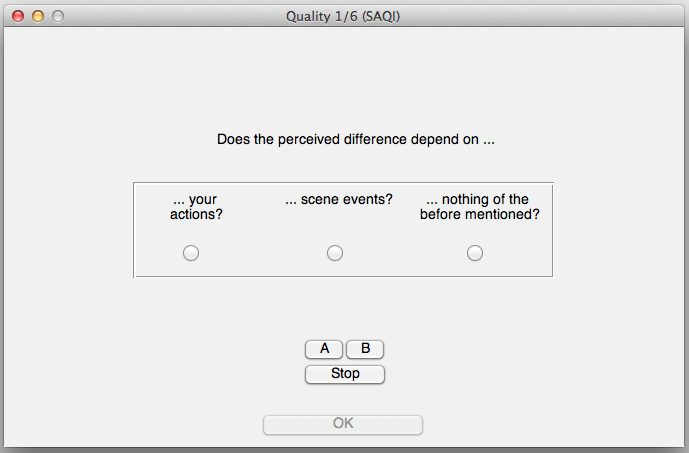
\includegraphics[width = 10cm]{saqi_modification_3.png}
 	\caption{GUI for the rating the cause of perceived differences}
  \label{fig:saqi_modification_3}
\end{figure}
\clearpage
% screenshoot entities %Alex: tippfehler by "back(g!)round sources', auf server bereits behoben, screenshot neu machen
\begin{figure}[!h]\centering
	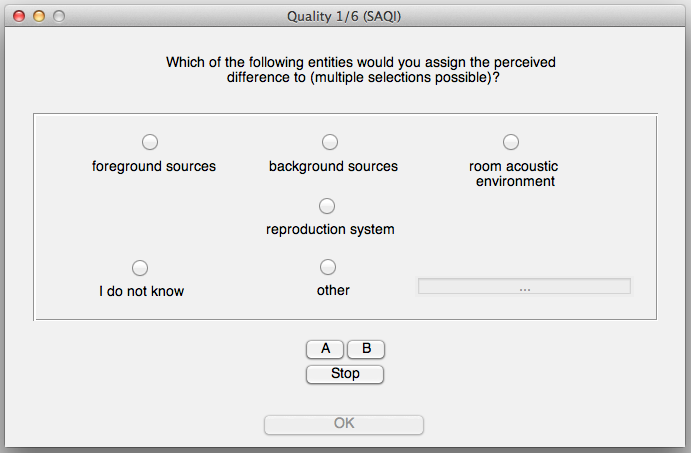
\includegraphics[width = 10cm]{saqi_entities.png}
 	\caption{GUI for assigning assessment entities to perceived differences}
  \label{fig:saqi_entities}
\end{figure}

% 7.5.2
\subsection{Setting up Properties \small{(Fig.~\ref{fig:saqi_editmain})}}\label{saqi_setup}
% figure
% Screenshot saqi_edit_main
\begin{figure}[!h]\centering
	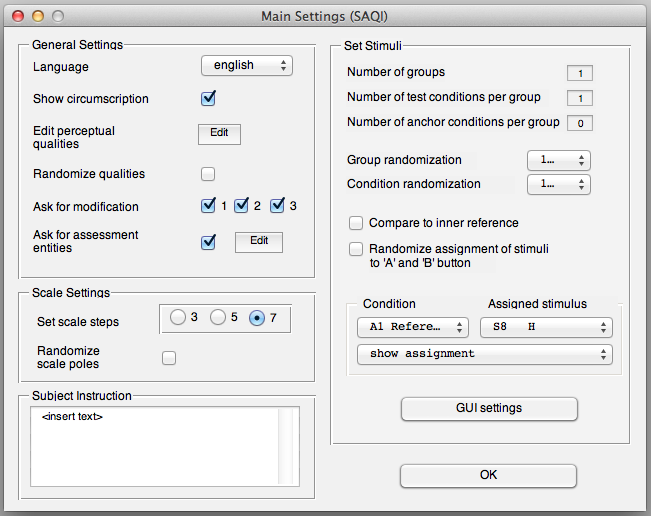
\includegraphics[width = 10cm]{saqi_main_settings.png}
 	\caption{SAQI Main Settings}
  \label{fig:saqi_editmain}
\end{figure}

% DW "General Settings (SAQI)"
\minisec{DW \itshape\lqq SAQI -- edit General Settings (panel)\rqq}\medskip
% language
\textbf{Language} (\textit{drop-down list})\\
As mentioned in the beginning, it is possible two choose between conducting SAQI tests in either German or English language. The default language is German. In programming the SAQI, possibilities have been foreseen for adding new languages. In case you plan to add a new national version of SAQI, please check section ~\ref{saqi_language}.

% Show circumscription (checkbox)
\textbf{Show circumscription} (\textit{check box})\\
Check to show the written circumscriptions of the perceptual qualities in a separate window before assessing each quality. The default setting is 'on'.

% Edit perceptual qualities
\textbf{Edit perceptual qualities} (\textit{push button}; Fig.~\ref{fig:saqi_quality})\\
Pushing the 'Edit' button opens another window for selecting the perceptual qualities. 
It contains all 48 original descriptors included in the SAQI. By default they are entirely selected. Furthermore, all qualities are 
subdivided in categories. \\
In order to customize a SAQI test, it is possible to either select singular qualities separately (left window pane) or to select entire categories (right window pane).
\medbreak
Please note, that the first ('overall difference') and the last quality ('other') \textbf{must} be selected, otherwise a warning window will pop up, telling you to do so. If qualities are chosen by selecting complete 'categories' (right window pane), these two qualities are selected automatically. The 'De/Select all' button enables you to select or de-select all (also including both, the first and last) qualities. 

% figure edit_qualities
\begin{figure}[!htbp]\centering\label{saqi_quality}
	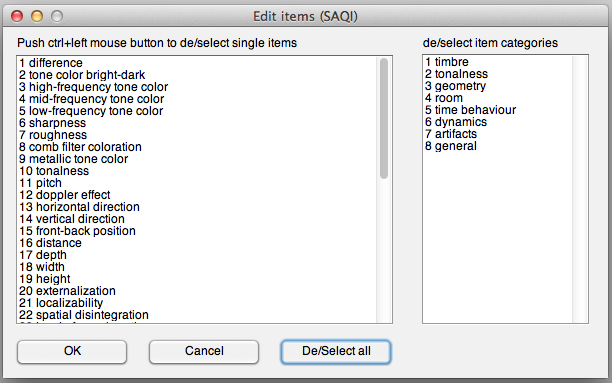
\includegraphics[width = 10cm]{saqi_edit_qualities.png}
 	\caption{GUI for the selection of perceptual qualities. Left: singular selection, right: category-based selection.}
	 \label{fig:saqi_quality}
\end{figure}
	
% Randomize qualities (checkbox)
\textbf{Randomize qualities} (\textit{check box})\\
Randomizes the selected perceptual qualities during test presentation according to the following scheme: Firstly, the order of categories is randomized, and secondly, the order of qualities within the categories. Exceptions are again the first and the last quality, which will be invariably presented at first and last position, respectively.

%% Ask for categorization
\textbf{Ask for modification} (\textit{check boxes})\\
(Only available for single condition/stimulus SAQI, see sec.~\ref{saqi_conditions})\\
By default, all three types of modifications a pre-selected (checked) for assessment. Please note, that modification 2 depends on modification 1. Hence, if modification 1 is disabled for assessment, modification 2 will automatically be disabled, too. Modification 2 cannot be chosen for exclusive assessment.\\
\begin{enumerate}
	\item modification 1 (temporal variation): constant/varying periodically or otherwise 
	rule-based/varying non-regularly
	\item modification 2 (temporal variation): continuous/discontinuous
	\item modification 3 (causality): depending on scene events/depending on user interaction/independent
\end{enumerate}

% Ask for assessment entities
\textbf{Ask for assessment entities} (\textit{check box / push button}; Fig.~\ref{fig:saqi_edit_entities})\\
(Only available for single condition/stimulus SAQI, see sec.~\ref{saqi_conditions})\\
By pushing the 'Edit' push button it is possible to define five entities a perceived difference may be further ascribed to. 
If needed, the default ones can be overwritten. Furthermore, the entities can be selected exclusively by the check boxes to the left. The last two entities 'I don't know' and 'other' cannot be renamed. By default, all entities are enabled.

% figure entities setup
\begin{figure}[h]\centering\label{saqi_edit_entities}
	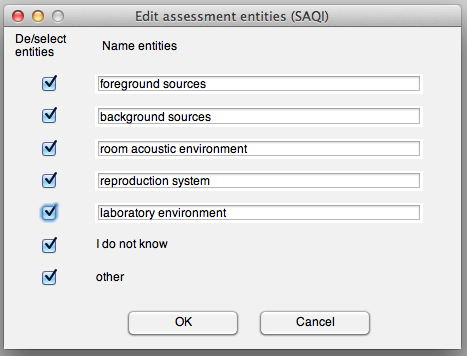
\includegraphics[width = 10cm]{saqi_edit_entities.png}
 	\caption{Default assessment entities}
	\label{fig:saqi_edit_entities}
\end{figure}

% DW " SAQI - Scale settings"
\minisec{DW \itshape\lqq SAQI -- Scale settings (panel)\rqq}\medskip

% Set scale size
\textbf{Set scale steps} (\textit{radio button})\\
The user can choose between the scale steps '7', '5' and '3'. The default setting is '5'. Scale steps only refer to the bipolar and unipolar qualities.\\
For example: A bipolar scale with '7' steps will range from +/-3, where 0 marks the middle ('no difference'). At the same time, an unipolar scale will range from 0 to 3, enabling to encode the \textbf{amount} of a perceived difference, only, and not its \textbf{direction}.

\textbf{\emph{Important note:}} Please note that scale steps are intended only as visual guidance for test subjects. Internally, all ratings will always be coded in a range of -1 to +1 in floating point resolution independent of the chosen number of scale steps to be displayed.

% Randomize scale poles (check box)
\textbf{Randomize scale poles} (\textit{check box})\\
Check to randomize scale orientation and corresponding label while test presentation. The default setting is 'off'. During default setting scales are arranged in a way that perceived increases are 'logically' encoded by moving a slider upwards. The label, that is listed first in the definition file \emph{saqi\_scale\_label\_language.m} is coded with $-1$ (bipolar/dichotom/degree quality) or $0$ (unipolar quality), regardless of randomization. The label that is listed in second place always is coded with $+1$. Hereby, throughout the whole SAQI the logic was followed to orient scales by default in a way that positive values may intuitively related to a perceived increase of the respective quality. Hence, as an example, a positive rating value of the \textit{distance}-quality indicates an increase in perceived distance, or, as another example, for the \textit{sound color}-items positive values will naturally indicate perceived amplifications/boosts.

% DW " SAQI -Subject instruction"
\minisec{DW \itshape\lqq SAQI -- Subject instruction (edit text field)\rqq}\medskip

% Subject instruction
Space for entering terms of instructions that will be displayed on the subject's \textit{basic screen} (see sec.~\ref{testrun}) before the test section is started.

% DW " SAQI -Set stimuli (panel)"
\minisec{DW \itshape\lqq SAQI -- Set stimuli (panel)\rqq}\label{sec:saqi_set_stimuli}\medskip

% Test conditions
\textbf{Number of groups, test and anchor conditions} (\textit{text edit fields})\label{saqi_conditions}\\
These three parameters can be used to define the number and kind of test conditions. Their behaviour is best explained by three examples:
\begin{enumerate}
\item Single stimulus SAQI
	\begin{itemize}
	\item[] One test/comparison stimulus is compared to a given or imagined reference, see Tab.~\ref{saqi_conditions},~(1). For example a binaural simulation (comparison stimulus) could be compared to the sound field of a loudspeaker (reference). In this case on slider will be displayed per rating screen and modifications and assessment entities can be included in the test (see above).
	\end{itemize}
\item Multiple stimuli, single group SAQI
	\begin{itemize}
	\item[] Multiple test/comparison and anchor stimuli are compared to a given or imagined reference, see Tab.~\ref{saqi_conditions},~(2). For example, auralizations obtained from different room acoustic modeling algorithms (test conditions) could be compared to binaural recordings (reference), while also providing an auralization using a monaural room impulse response (anchor). In case the number of test conditions, plus the number of anchor conditions is larger than nine, ratings will be split among two or more rating screens. The anchor condition(s) will be provided on every rating screen, however only the last rating of each anchor conditin will be saved.
	\end{itemize}
\item Multiple stimuli, multiple groups SAQI
\begin{itemize}
	\item[] Groups of multiple test/comparison and anchor stimuli are compared to given or imagined references, see Tab.~\ref{saqi_conditions},~(3). To understand hza is meant simply expand the example given above (2) for similar conditions but using, say, two different audio contents (groups). If one group contains more than four conditions (test plus anchor), only one group will be displayed per rating screen.
	\end{itemize}
\end{enumerate}

% table entities setup
\begin{longtable}{p{4cm} c c c}
\multicolumn{1}{l}{\textbf{Parameter}} &  \multicolumn{1}{c}{\textbf{(1)}} &  \multicolumn{1}{c}{\textbf{(2)}} &  \multicolumn{1}{c}{\textbf{(3)}}\vspace{.1cm} \endhead\hline
Number of groups					&1	&1	&2	\vspace{.2cm}\\
Number of test conditions per group		&1	&6	&3	\vspace{.2cm}\\
Number of anchor conditions per group	&0	&1	&1	\\
\hline
\caption{Exemplary parameters for obtaining different SAQI modes: (1) Single stimulus; (2) Multiple stimuli, single group; (3) Multiple stimuli, multiple groups}
\label{saqi_emp_data}
\end{longtable}

% Group/condition randomization
\textbf{Randomization of groups and conditions} (\textit{drop-down list})
\begin{enumerate}
\item none --- Groups and conditions are presented in the order specified by the investigator.
\item per subject --- Groups and conditions are randomized per subject, but their order remains identical across auditory qualities.
\item per quality --- Groups and conditions are randomized per subject and quality. Note that in this case the subjects have to listen to each stimulus for each auditory quality before being able to rate (sliders are disable beforehands).
\end{enumerate}

% Compare to inner reference
\textbf{Compare to inner reference} (\textit{check box})\\
Check this option to allow the user to rate the test stimulus against his/hers inner reference. In this case, the second play button and stimulus will be omitted in the respective GUIs and GUI instructions will be reformulated accordingly. Refer to the SAQI Test Manual \cite{lindau:2015} for hints towards a proper test subject instruction.

% Randomize Assignement of stimuli to 'A' and 'B' button (checkbox)
\textbf{Randomize Assignment of stimuli to 'A' and 'B' button} (\textit{check box})\\
Check to randomize assignment of the the stimuli 'A' and 'B' to play buttons when assessing the next perceptual quality. In this case, the subject must listen to the stimuli before being able to rate the current quality. This will noticeably increase the test duration. If stimuli are randomized, the rating is decoded by switching the sign, and thus, the effect of randomization is compensated in the rating. 

% Stimulus assignment across conditions
\textbf{Stimulus assignment across conditions} (\textit{drop-down lists})\\
Stimuli from the global stimulus pool can be assigned to conditions by first selecting a condition from the top-left drop-down list and, second selcting a stimulus from the top-right drop-down list. The drop-down list at the bottom gives an overview of the current assignments (Fig.~\ref{fig:saqi_condition_assignment}). Stimuli are specified by their \emph{ID} and \emph{name} as specified by the investigator.
\begin{figure}[h]\centering
	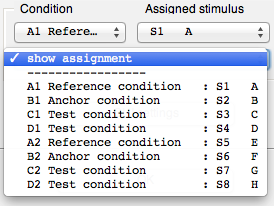
\includegraphics[width = 5cm]{saqi_condition_assignment.png}
 	\caption{Stimulus assignment across conditions}
	\label{fig:saqi_condition_assignment}
\end{figure}

% Stimulus assignment across conditions
\textbf{GUI settings} (\textit{push botton, text edit fields})\\
Controls the maximum and minimum number of conditions and groups to be displayed on each rating screen, and the positions of the scale labels (Fig.~\ref{fig:saqi_GUI_settings}). The latter was introduced to provide correct positions for various operating systems and Matlab versions. Only change these parameters if the default bahviour does not match your needs.
\begin{figure}[h]\centering
	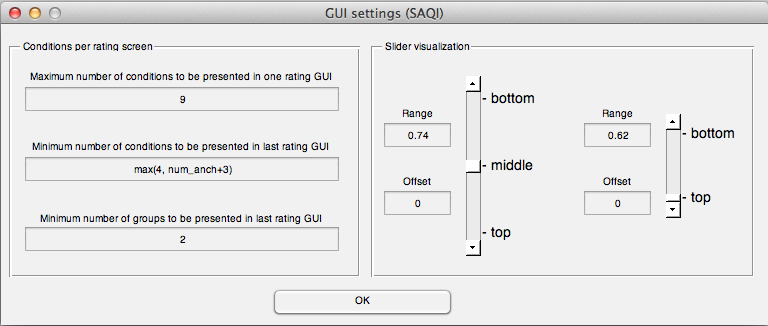
\includegraphics[width = 12cm]{saqi_GUIsettings.png}
 	\caption{Settings for distribution of conditions across rating screens.}
	\label{fig:saqi_GUI_settings}
\end{figure}

\subsection{How to: Implementing SAQI for a New Language}\label{saqi_language}

Adding a new language is possible, and the required steps are described in the following. However, this reconfiguration will need some understanding of Matlab and is not thought to be a normal usage procedure of \whisper. Hence, if you do not feel save with these requirements, please contact us for help. We can also - as a service - add national versions of SAQI to \whisper. In any case, please send us the new language files, so we can update the \whisper\ release on the project homepage.

\begin{description}
	\item[Step 1: Create new language files]  
\end{description}	
 As a first step, it will be necessary to re-create some of \whisper's Matlab scripts in your desired language, containing the names for:
	\begin{itemize}
		\item quality descriptors  (original example file: saqi\_items\_german.m),
		\item categories (original example file: saqi\_categories\_german.m),
		\item circumscriptions (original example file: saqi\_definitions\_german.m),
		\item GUI phrases (original example file: saqi\_phrases\_german.m),
		\item scale label ends (original example file: saqi\_scale\_label\_german.m),
		\item assessment entities (original example file: saqi\_entities\_german.m)
	\end{itemize}

The best way will be to copy the original (German or English) versions of these files at a save place and change them accordingly, one by one. The structure of these files is pretty straight-forward and may be checked out by retrieving them from the \whisper\ source code folder. Please note, that your new files need to be known in the Matlab's path environment (at best they are saved in the \whisper\ source code folder).

In case letters with accents occur in the implemented language please decode them as done in \emph{saqi\_scale\_label\_german.m} to ensure compatibility across different system and system locales. 
\\

\begin{description}
\item[Step 2: Adding a new language case to the setup GUI]
\end{description} 
Now, you should update the language selection switch of the setup GUI by adding another case for your language. You can find the program code in the \textit{saqi\_edit\_main file}. The switch is arranged in a function called 'pop\_language\_Callback' (line 365 et seq.).

The easiest way of adding, is to copy-and-paste one of the existing cases and to rename the applied m-files (e.g. saqi\_items\_french) in the new one (e.g. case 3).

\begin{description}
\item[Step 3: Additions on the GUI]
\end{description} 
For the last step you will need to edit the figure 'saqi\_edit\_main.fig', for example using the GUIDE-Tool of Matlab (right-click on the fig-file and choose 'open with GUIDE').\\
Next, double click on the language drop-down list in the panel 'General Settings' and a Matlab 'Inspector' will open. In this 'Inspector' it is possible to change settings. Open the edit-box by double clicking on 'String' an add your language under the last enlisted.\\

% ABCHR & MUSHRA
\section{ITU-R Rec. BS.1116-1 (ABC/HR) \& ITU-R Rec. BS.1534-1 (MUSHRA)}\label{sec:abchr_mushra}
ABC/HR and MUSHRA are methods for rating multiple conditions against one or more references. ABC/HR includes a detection task according to the ABX paradigm and should be used when differences between test and reference conditions are expected to be small, whereas MUSHRA is recommended for usage with intermediate differences.

\subsection{The Test Run}
The rating GUIs (Fig.~[\ref{fig:abchr_gui}, \ref{fig:mushra_gui}]) are subdivided in three parts:
At the top, the question stating the task for the subject is displayed. The middle part shows the sliders and text fields for rating the test conditions, as well as the play and stop buttons, and at the bottom, the ratings can be saved or reset.
Sliders and edit fields are initially disabled and will be enabled after the subject listened to the corresponding stimuli. The \emph{OK}-button will be enabled after the subject listened to all stimuli.

\begin{figure}[h]\centering
	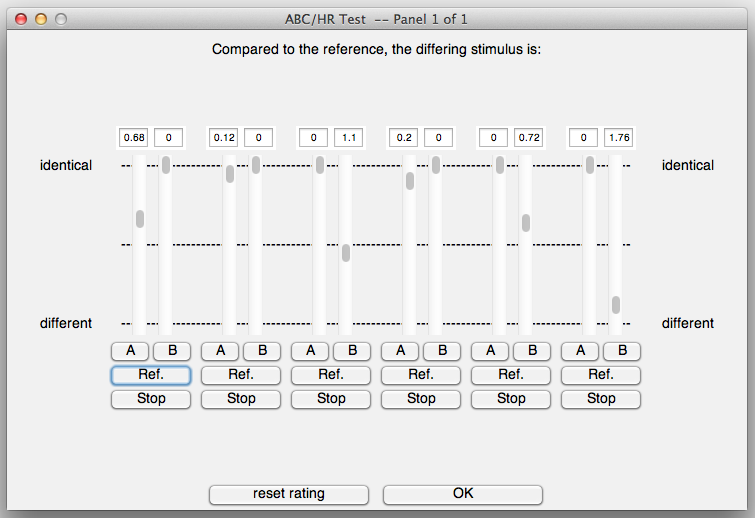
\includegraphics[width = 12cm]{abchr_gui.png}
 	\caption{ABC/HR rating GUI}
	\label{fig:abchr_gui}
\end{figure}
\begin{figure}[h]\centering
	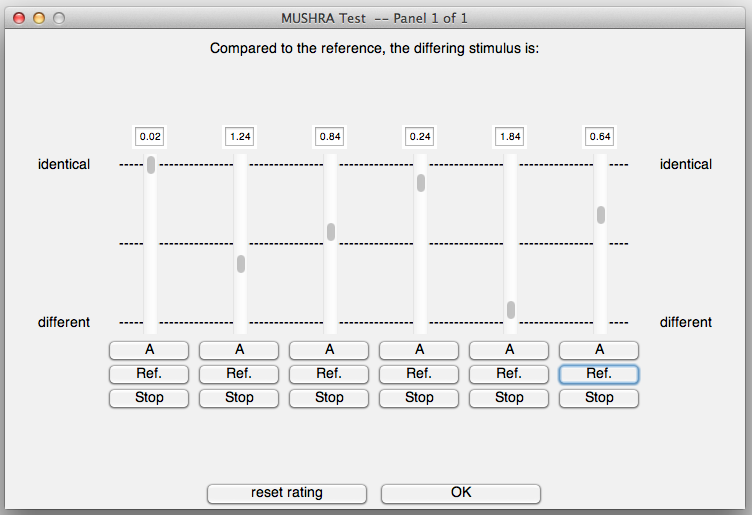
\includegraphics[width = 12cm]{mushra_gui.png}
 	\caption{MUSHRA rating GUI}
	\label{fig:mushra_gui}
\end{figure}

% ABCHR MUSHRA settings
\subsection{Setting up Properties \small{(Fig.~\ref{fig:abchr_mushra_settings})}}\label{abchr_mushra_setup}
\begin{figure}[h]\centering
	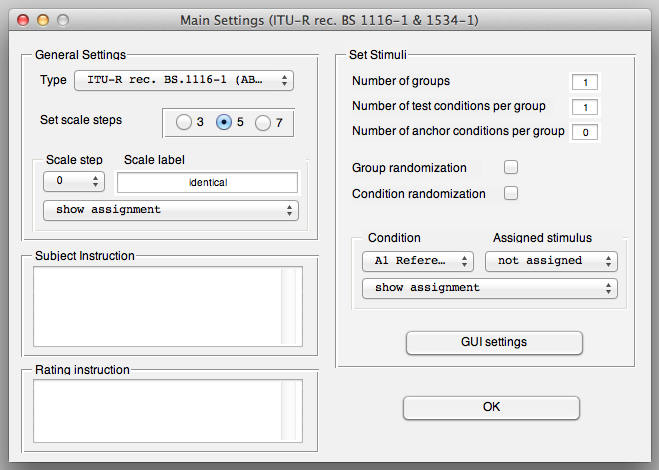
\includegraphics[width = 12cm]{abchr_mushra_settings.png}
 	\caption{ABC/HR and MUSHRA setting}
	\label{fig:abchr_mushra_settings}
\end{figure}

% DW "General Settings (ABCHR MUSHRA)"
\minisec{DW \itshape\lqq ABC/HR \& MUSHRA -- edit General Settings (panel)\rqq}\medskip
% language
\textbf{Type} (\textit{drop-down list})\\
Choose \emph{ITU-R Rec. BS.1116-1 (ABC/HR)} or \emph{ITU-R Rec. BS.1534-1 (MUSHRA)} depending on your needs. Thill will affect the layout of the rating screen (see Fig.~[\ref{fig:abchr_gui}, \ref{fig:mushra_gui}]).

% Set scale size
\textbf{Set scale steps} (\textit{radio button})\\
The user can choose between the scale steps '7', '5' and '3'. The default setting is '5'. A scale with '7' steps will have seven eqidistant markers wich can be individually labeled (see below).\\
\textbf{\emph{Important note:}} Please note that scale steps are intended only as visual guidance for test subjects. Internally, all ratings will always be coded in a range of -1 to 0 (MUSHRA), and -1 to +1 (ABC/HR) in floating point resolution independent of the chosen number of scale steps to be displayed. In both cases, '0' denotes that the subject perceived no difference, i.e. the sliders were not moved, and '-1' denotes a large difference, i.e. the slider was moved all the way down. In case of ABC/HR, positive numbers indicate the the subject failed to detect the reference, i.e. the subject moved the wrong slider.
 
 % Scale label assignment
 \textbf{Scale label assignment} (\textit{drop-down lists \& text edit field})\\
Individual labels can be assigned to the scale markers, by selecting a marker using the top left drop-down list and writing the label into the edit field on the top right of the panel. The drop-down list at the bottom can be used to show the currently assigned label.\\
\textbf{\emph{Note}} that the default label ('identical', and 'different') differ from the suggestions made by the ITU (ABC/HR: 'Imperceptible', 'Perceptible, but not annoying', 'Slightly annoying', 'Annoying', 'Very annoying'; MUSHRA: 'Excellent', 'Good', 'Fair', 'Poor', 'Bad'). This was done because the ITU suggestions are believed to be multi-dimensional (i.e., mixing evaluative and magnitude related connotations) and non-equidistant and therefore possibly bias the test results.

% DW "Instructions (ABCHR MUSHRA)"
\minisec{DW \itshape\lqq ABC/HR \& MUSHRA -- instructions (panel)\rqq}\medskip
\textbf{Subject Instruction} (\textit{text edit field})\\
Use this to specify the instructions that subjects will read before rating.

\textbf{Rating Instruction} (\textit{text edit field})\\
This is the question that will be displayed at the top of the rating GUIs (Fig.~[\ref{fig:abchr_gui}, \ref{fig:mushra_gui}]).

% DW "Set stimuli (ABCHR MUSHRA)"
\minisec{DW \itshape\lqq ABC/HR \& MUSHRA -- set stimuli (panel)\rqq}\medskip

For \emph{Number of groups, test and anchor conditions}, \emph{Stimulus assignment across conditions}, and \emph{GUI settings} see Sec.~DW {\itshape{\lqq SAQI -- Set stimuli (panel)\rqq}} on page~\pageref{sec:saqi_set_stimuli}.

\textbf{Group randomization} (\textit{check box})\\
If enabled, the presentation order of groups will be randomized. Elsewise, the presentation order will be as specified.

\textbf{Condition randomization} (\textit{check box})\\
If enabled, the presentation order of conditions (text, and anchor) will be randomized. Elsewise, the presentation order will be as specified.

\clearpage
%-----------------------------------------
% CHAPTER 8
%-----------------------------------------

\chapter{Test procedures - Default Values' Presets}\label{defaults_presets}
This section is about a feature of \whisper\ that allows the user to manipulate all the procedures' default values (as they are mentioned in chap.\,\ref{testprocedures}), which the procedures are initialized with upon adding them to a test series via the test section setup (cf.\,sec.~\ref{edit_testsections}).

The DW that allows you to do this is accessible via the main window's menu \textit{edit\textbackslash procedure's defaults}.

\begin{figure}[h]\centering
        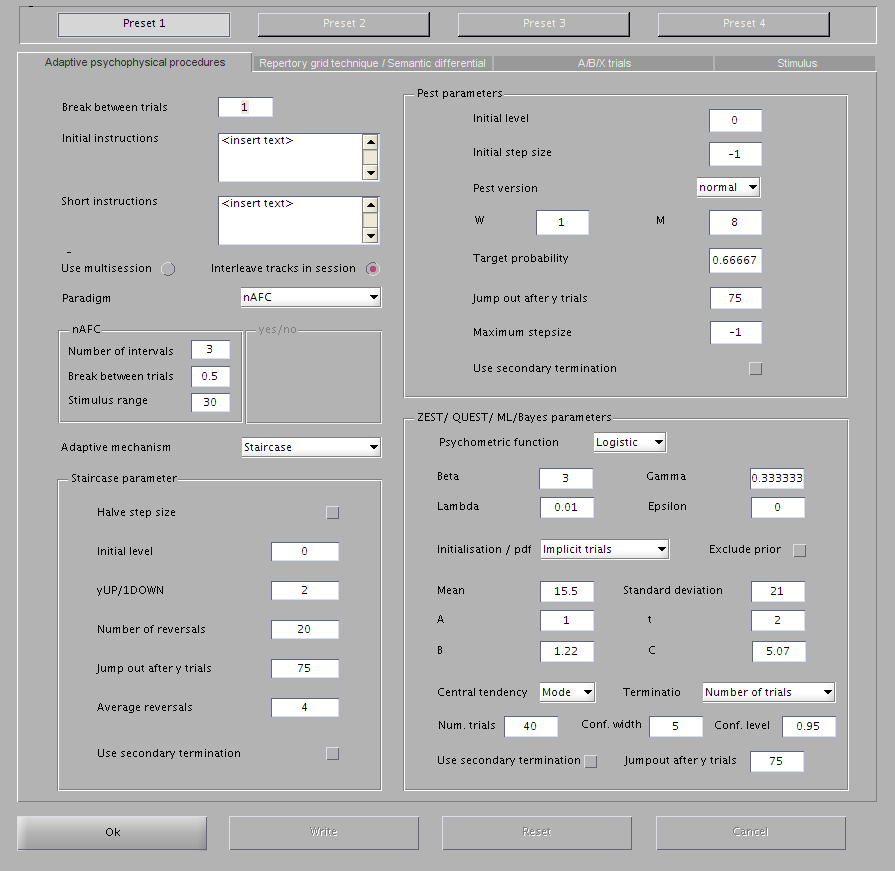
\includegraphics[width = \textwidth]{procedures_defaults1.png}
        \caption{DW \textit{Configure defaults' presets}}
  \label{fig:procedures_defaults1}
\end{figure}

This DW consists of a middle part comprising four  \textit{tabs} containing all the configurable default values for all the procedures (plus for the stimuli), a lower part consisting of four \textit{buttons} for closing, writing, resetting and canceling your configurations and an upper part consisting of four \textit{preset buttons}, each selecting one of four presets. Following that order the description in detail:

\begin{description}
  \item[Adaptive psychophysical threshold procedures] (\textit{tab}) This \textit{tab} contains spaces for all the configurable defaults of the  parameters of the AP procedures as explained in sec.~\ref{ap_setup}. 

Please note: As stimulus definitions take place separately from procedure setup (cf. sec.~\ref{stimuli} and \ref{edit_testsections} of chap.~\ref{settingup_testseries}) all AP configuration options involving (already defined) stimuli in any way (e.\,g.\ stimulus assignments to intensities or reference level) sensibly simply cannot be available here. They have to be set later. 

Please also note that as this DW is intended for the power user all the input fields are presented in a condensed and often abbreviated way, thus lacking the guidance of the DWs of the \textit{in procedure setup} as in sec.~\ref{ap_setup}, but instead allowing all the options to be set in one window only in the flattest hierarchy and the fastest way possible. Please note again that changing values here will of course not disable you from making changes later, after adding a procedure to your test series -- changing values here will only affect the values your procedure \textit{already has} just after you have added it.
Thus it is perfectly possible to just once set those values here that are most likely to \textit{not} change from listening experiment to listening experiment (like for example the psychometric function or the a priori p.\,d.\,f.\ or the number of trials etc.) and thus are always initialized to \textit{your} defaults, and later fill in those values that are specific to a single listening experiments (like e.\,g.\ the participants' instructions).

Of course you can also use this DW to just make all your wanted changes for one specific listening experiment in case you simply prefer the availability of all the configuration options in one place without having to click through multiple configuration DWs.

  \item[Repertory grid technique / Semantic differential] (\textit{tab}) This \textit{tab} contains spaces for all the configurable defaults of the  parameters of the RGT procedure as well as the SD procedure as explained in sec.~\ref{rgt_setup} and in sec.~\ref{sd_setup} respectively. For notes and hints please see above.

  \item[A\,/\,B\,/\,X trials] (\textit{tab}) This \textit{tab} contains spaces for all the configurable defaults of the  parameters of the ABX procedure as explained in sec.~\ref{abx_setup}. For notes and hints please see above.

  \item[Stimulus] (\textit{tab}) This \textit{tab} contains spaces for all the configurable defaults of stimuli (cf.\,sec.~\ref{stimuli}), see fig.~\ref{fig:procedures_defaults2}.  Notes and hints above also apply here, further explanation  see below.
    \begin{description}
      \item[New Stimulus default name] (\textit{input field}) Space for entering what is to be the default name of a stimulus each time one is created either by pushing the \textit{new button} or the \textit{multi new button} in the stimulus pool DW (as explained in sec.~\ref{stimuli}). As changing this from " - no name - " to whatever you desire will effectively \textit{inhibit}\ automatic name generation for stimuli based on a .wav file name, this will only be useful under two conditions: First, when you just do not want your stimuli to be named corresponding to the .wav files loaded, and second, when there are no .wav files to be loaded to begin with, i.\,e.\ your stimuli are OSC only. Please be advised, that in both cases the name entered here will only be a "base name", as it will result in the \textit{same} default name for every stimulus generated. With that "base name" already filled in the stimulus' name field, however, individualizing each name by simply manually appending a number, for example, is facilitated a lot. Cf.\, below for OSC usage scenarios.
        \item[New Stimulus default OSC data] (\textit{panel}) Contains spaces for entering what is to be the default OSC parameters of newly generated stimuli. As explained above for the \textit{New Stimulus default name} the values entered here will result in  exactly the \textit{same} default OSC data values for every stimulus newly generated. Thus their use is to serve as "base parameters", with later only individual addition of e.\,g.\ numbers in the \textit{OSC data field}\ for each stimulus facilitating the creation and configuration of a bigger set of OSC only stimuli.
\end{description}
\begin{figure}[h]\centering
        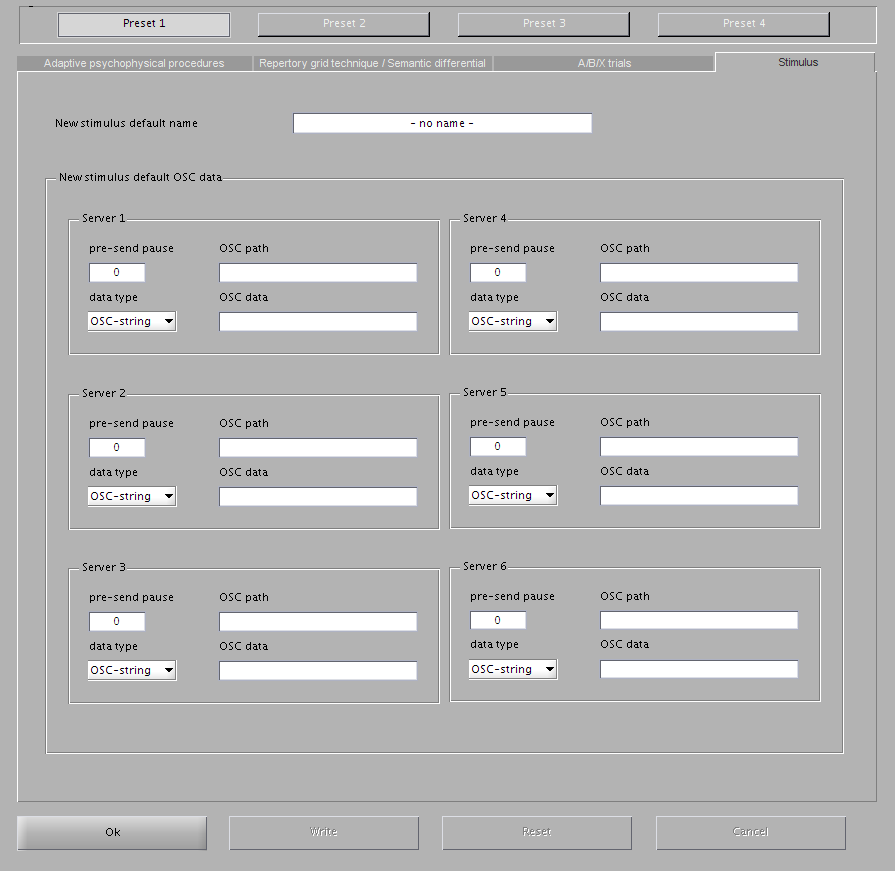
\includegraphics[width = \textwidth]{procedures_defaults2.png}
        \caption{DW \textit{Configure defaults' presets} -- tab "Stimulus"}
  \label{fig:procedures_defaults2}
\end{figure}
\item[Ok] (\textit{button}) This \textit{button} will save your changes and close the DW. Please note that "saving your changes" means making them immediately effective (for the addition of test procedures for example) as well as storing them so they stay the way you configured them even over the course of exiting the program (\whisper\ as well as MATLAB\circledR\ ) and starting it again.
\item[Write] (\textit{button}) This \textit{button} will save your changes and leave the DW open. Again "saving your changes" means making them immediately effective (for the addition of test procedures for example) as well as storing them so they stay the way you configured them even over the course of exiting the program (\whisper\ as well as MATLAB\circledR\ ) and starting it again. 

The purpose of \textit{not} closing the DW but making your changes effective is the following: 
You might have noticed that when you open the \textit{Configure defaults' presets} DW it does not force the main program window to disappear or close. As the addition of a test procedure to a test series (or a test section respectively) or stimuli to the pool are not done in the main window but "some DWs away", having to go back and forth after changing the defaults and wanting to add a test procedure would result in a lot of unnecessary clicking. So instead the \textit{Configure defaults' presets} DW stays open after pushing \textit{Write}, all changes are effective, you navigate to e.\,g.\ the test section setup and add a procedure and you can still change the defaults  in this still open DW, push \textit{write} again and your new defaults are immediately in effect again. 
\item [Cancel] (\textit{button}) This \textit{button} will close the DW  discarding your changes -- neither will they come to effect, nor will they be stored for later. Please note that the state of this \textit{button}\ will also signal to you if changes have been made at all -- it will only be enabled if they have.
\item [Reset] (\textit{button}) This \textit{button} will reset the values and selections in all the above explained four \textit{tabs} -- which constitute the current  preset (see below) -- to the values originally intended by the programmers of \whisper\ and made available to you when you first got the software (as introduced above in sec.~\ref{ap_setup}, sec.~\ref{rgt_setup}, sec.~\ref{sd_setup} and sec.~\ref{abx_setup}). The reset values will also be immediately effective and will be stored for later, too -- this means a "Reset" action cannot be canceled via the \textit{Cancel button}!
Please note that the state of this \textit{button}\ will also signal to you if the values in the current four \textit{tabs} differ at least in one respect from the original provided ones  -- it will only be enabled if they do.
\item [Preset 1-4] (\textit{buttons}) These \textit{buttons} select one of the corresponding four presets. A preset comprises \textit{all}\ values and selections of \textit{all the four tabs}, and not just the momentarily visible one. So preset 1 has a tab for AP, a tab for RGT/SD, a tab for ABX and a tab for stimulus, and these four \textit{make}\ preset 1, preset 2 has a tab for AP, a tab for [\dots] and so on. Changing tabs and entering values will only affect the \textit{current} preset, symbolized by the preset button at the top that is pushed. Pushing \textit{Ok}, \textit{Write} and  \textit{Reset} will also only act on the current selected preset \footnote{And \textit{Cancel} will actually "act" on nothing}. Changing presets by pushing a different preset button at the top will do two things: a) It will always store the preset you are leaving for later (this means you cannot have unsaved changes over the course of a preset change),  and b) it will make the newly selected preset immediately effective. 

This preset system can be used in an even more refined way than what was described above along with the \textit{Write button}: Leaving the \textit{Configure defaults' presets} DW open in the background and having configured two presets differing e.\,g.\ only in the types of the adaptive mechanism and their corresponding settings, it is easily possible to first select one of those presets, add a new track to your AP test section, then select the other preset and just again add a new track -- thus with just four clicks you really quickly generated two tracks containing the same procedures, albeit with totally different settings -- enabling e.\,g.\ the comparison of different adaptive mechanisms.

Previously unaltered presets default to the initial defaults (cf.\,above, (\textit{Reset button}), presets stay persistent over the course of exiting the program and opening it again, and the choice of which preset is currently active is persistent to ending the program and starting it up again, too. 

Presets are stored each in a file in the program folder, named PC.1.mat to PC.4.mat, these files are only generated when that preset has been selected at least once.\footnote{The original defaults are present in the file PC.mat, this should better not be touched.}
\whisper\ will not crash if one or even all of the PC.\textit{n}.mat is missing -- even if that preset had been the selected one -- but will simply generate a new one as a clone of the original defaults values. \footnote{Should you wish to use more than the provided four presets, you could thus simply move (or rename) your configured PC.\textit{n}.mat files and later exchange them or put them back -- \whisper\ will read them as if they had never been elsewhere.}
\end{description}
\clearpage



%-----------------------------------------
% CHAPTER 9
%-----------------------------------------

\chapter{Program Setup}\label{program_setup}
In this chapter the approach of adjusting the \textit{program settings} will be described. These refer to technical properties which are mostly independent of methodical issues and stored in the file \textit{PS.mat} which will be described in section~\ref{psmat}. 

\section{Basic Audio Setup}\label{audio_setup}
As \whisper\ currently uses the internal MATLAB\circledR\ function audioplayer, there are no general audio properties to be set.

\section{Basic Network Setup}\label{basic_network}
Basic network settings can be specified by selecting the item \textit{program setup\textbackslash network} from the menu bar. Then a DW will appear for entering host names or IP addresses respectively and port numbers of up to 6 OSC-servers. Each server is related to a single parameter which has to be determined when defining the stimuli's contents (see sec.~\ref{stimuli}). As in some cases one might want to address several parameters on one server, the servers need not necessarily be different. Note that the order in which the servers are defined has to be the same as the order in which the respective OSC-commands should be executed.
\clearpage




%-----------------------------------------
% CHAPTER 10 
%-----------------------------------------

\chapter{Data Handling}\label{data}
In this chapter basic information about the program's data structure will be provided as far as it is required to make use of the functionalities implemented. The aim is not to give a complete description which one needs to make modifications or to work on upgrades or kind of these things. For the latter purposes one is directed to the \textit{technical documentation} (see sec.~\ref{doc}). There are basically two kinds of data sets which may be accessed by the user. One contains all data belonging to a certain test series and is represented by the test series folder which may be placed at an arbitrary location (cp. sec.~\ref{create_testseries}). The second data set is contained in the file \textit{PS.mat} which is located in the program folder \lq 2 mfiles\rq\ and consists of global program settings (cp. chap.~\ref{program_setup}). Moreover there is a sub folder containing this user documentation.

\section{The Test Series Folder}\label{testseries}
This folder is quite essential to know for the user as it contains both the test series' empirical data set and its setup including audio data. In the following subsections the several files and subfolders, which will be automatically generated if a new test series is created, are described.

\subsection{The File \lq testseries.info\rq} This file contains information about the configuration of the test series and may be regarded as a documentation of the test series setup that should enable the user to understand the information provided by the log files or the export sheets. This information can be summed up by the following aspects:
\begin{itemize}
	\item Global settings: What stimuli have been defined? How many sessions have been set?
	\item Decoding of test section key numbers: What are the label names? What type of test procedure is used in each test section?
	\item Properties of the test procedures: How are stimuli grouped and assigned to single test units (elements, objects, triads, tracks)? What scales (format/labels) have been defined? (RGT/SD) Which response paradigm and which adaption mechanism have been selected? (AP)
	\item Decoding of session key numbers (experimental conditions): What subsets of test units have been selected and what sequences have been defined (manually defined vs. random sequences)?
\end{itemize}
\textbf{Note:} The file also serves as an identifier whose existence is a premise for the test series folder to be accepted as such by the program.


\subsection{The Files \lq TSD.mat\rq\ and \lq TSP.mat\rq}\label{tsdmat}
These two files constitute some of the program's most important internal data storages which in general should be handled with great care and therefore not be manipulated by the common user. Though there are a few exceptions which can be applied to simplify the experimenter's life and which, besides a short general description of the files' contents, will be noted in the following two paragraphs.

\paragraph{TSD.mat (\lqq test series data\rqq)} In this file all so far collected empirical data (i.e. more precisely the contents of the dependent variables which are to be exported) are stored. The only occasion for the common user to manually access this file is when one wants to clear all these data or remove them from the test series. This might be necessary either if one wants a kind of \lqq virginal\rqq\ test series folder (e.g. for replication of the test series) or if one wants to reset the counter of the current test run (i.e. more precisely of both the counters of the latest completed and the next test run) in order to be able to make some changes on the test series' setup after the latter has already been completed (cp. chap.~\ref{settingup_testseries}). The task at hand will be performed by deleting the file TSD.mat or at least moving it to a location outside the test series folder if one wants to preserve the data. Additionally it is recommended to clear the contents of the sub folders \textit{plot}, \textit{export} and \textit{logfiles}. Otherwise this could lead to confusion as old and new files will be mixed and old files might be gradually overwritten (not in general but in most cases if old and new files carrying the same labels). Do not forget also to make a copy of the folders' contents if you want to preserve the data.
% Martina 
\subparagraph{Important Note on SAQI!} 
Please note, that as referring to the previous paragraph SAQI-tests resemble an exception. In case of SAQI tests the TSD.mat should NOT be deleted, because it contains all empirical data collected from all subjects so far! Instead, it should be saved after every test run in another folder to avoid loosing collected data. As already stated in section ~\ref{settingup_testseries} you can find the TSD.mat in the current test series folder.


\paragraph{TSP.mat (\lqq test series properties\rqq)}
Here all data concerning the test series' setup are stored. In the standard case it is not necessary for the user to manually access this file, as the setup normally is performed by using the GUI system (see chap.~\ref{settingup_testseries}). Anyhow in some cases it might be necessary to export these configuration data to another test series folder if it is desired to use a quite similar set up there. This can be done by copying the \textit{TSP.mat} to the destination test series folder and replacing the local file with it. Note that in such a case one also has to copy the folder \textit{audio} if the files in it should be played.


\subsection{The Subfolder \lq audio\rq}\label{audio}
This subfolder contains the audio files which are copied to there by the program in the context of the stimuli's definition (cp. sec.~\ref{stimuli}). Note that once an audio file has been uploaded, it will not be deleted at a later time even if it is no longer used at a certain point. Of course, in the latter case this may be manually done in order to save storage space. Note furthermore that files all must have different names as otherwise the program will not be able to distinguish between them and errors will occur. This can be ensured by using the GUI system to define the stimuli. If then a .wav file of the same name already exists it will be overwritten.


\subsection{The Subfolder \lq export\rq}\label{subfolder_export}
This subfolder contains the \textit{export sheets}, i.e. text files that include all so far collected empirical data (i.e. more precisely the contents of the dependent variables which are to be exported). The export sheets are saved as .csv files and therefore may directly be opened by the spreadsheet software Excel. They can also be imported to the statistical evaluation software SPSS\footnote{Tested on version 15.0. Note: Use the menu item \lqq Read text data ...\rqq\ and select the option \lqq All Files (*.*)\rqq\ from the drop-down list in the file dialog to make .csv files visible.}. Each file includes the data of a certain test section across all runs. Therefore there are as much files as there have been test sections defined in a test series and the information provided by a file's name only consists of the section number. After each run the export sheets are updated by being created anew. This can also be done manually at any time by using the menu item \textit{test series\textbackslash export empirical data} (see sec.~\ref{menubar}).

The internal structure of an export sheet is constituted in the following way. Each line represents the data belonging to a different run. Lines are sorted in ascending run numbers. Each column comprises a different variable's values. The first line includes the column labels, i.e. the variables' names in an abbreviated format. Columns are separated by semicolons. The first variable always is the run number, the second is the subject id and the third the session key number. Further variables and columns respectively depend on the specific type of test procedure applied. They will be stated in the following three paragraphs (see also fig.~\ref{fig:exportsheets}).\label{export_var}
% Martina
\subparagraph{Important Note on SAQI!} 
Please note, that in case of an SAQI test run the previous explanation is not valid. For extracting the empirical data please look up the paragraph about SAQI in this section.

\paragraph{Adaptive Psychophysical Threshold Procedures} For an AP the dependent variable is the threshold value estimated in the end of each track. As there may be several tracks defined, i.e. if tracks are interleaved and/or performed under different experimental conditions (i.e. assigned to different sessions), each column comprises the threshold estimates of all the test runs but for a different track. So if the number of tracks is given by $T$, there will be $T$ additional columns reserved. Thereby  columns are arranged by ascending track numbers. Note that there may be empty entries because not every track necessarily has to be performed in every run. In many applications there is only one track defined and performed by each subject, so that there is only one dependent variable and one additional column respectively in the export sheet.

\paragraph{Repertory Grid Technique} For the repertory grid technique there are two groups of elicited data: the first is of a qualitative format and constituted by the elicited constructs, the second is numeric data and consists of the ratings. Considering the first, the number of elicited constructs depends on the test run. For each construct there are two verbal descriptors --~ one for the high pole and one for the low pole\footnote{Only those constructs which have been used for rating, i.e. those that passed the editing in between the two parts of the procedure,  will be exported. Because the information about whether a descriptor evolved from either a similarity or a contrast between elements is lost, we do not speak of \textit{initial} and \textit{contrast pole} anymore.}. So if $C$ is the maximum number of constructs which has been reached in a run at all, there will be $2 \cdot C $ columns reserved for the storage of the verbal descriptors. Moreover if E is the total number of different elements involved in the rating process at all, there will be $E \cdot C$ further columns reserved for storing the rating values.

\paragraph{Semantic Differential} For the semantic differential the elicited data consists of numerical values evolved from the ratings. If $O$ is the total number of objects involved and $S$ is the number of items (i.e. scales), then $O \cdot S$ columns will be reserved for the storage of the dependent variables' values.

\paragraph{ABX Test} As results from the ABX test only the number of correct answers will be exported. \textbf{Please note}: The absolute number of trials per condition is not exported! This means, that, for later statistical analysis you will have to note this number by yourself! 
The number of correct answers will be saved in 4th column in the export sheet, i.e. in the row of the corresponding subject.
% Martina
\paragraph{SAQI} The internal structure of an SAQI-TSD-file is constituted in two levels. On the first level one can find information about the run number, the subject ID, the session number and the subject data. The second level is located in the fourth column named 'Subject Data'. There, you will find the elicited ratings in a 49x30xN cell. Each line in this cell represents the rating of one perceptual quality. Even if a quality/modification/entity was not included or rated one will find an entry about it. N equals the number of test conditions (see table ~\ref{saqi_emp_data}). \

\textbf{Important note on encoding of SAQI results!}\\
When saving SAQI results, these are always encoded as if being assigned to the stimulus under test when compared to the reference stimulus. This direction of encoding is also retained in saved results, if test and references stimuli are chosen to vary randomly for each assessed perceptual quality. Further, ratings are encoded to reflect perceived differences according to a logical increase of the quality under test. Thus, raw SAQI ratings may be interpreted intuitively: Positive difference ratings in terms of perceived high frequency coloration, sharpness, distance or clarity etc. refer to a perception of increase distance, emphasized high frequencies and a sharper, more distant and more clear sound of the test stimulus as compared to the reference. \

In case of an open-ended bipolar or a unipolar quality the value of the slider will be suitably transferred. In order to maintain an identical representation of values in the TSD.mat, in the case of the two bipolar qualities with closed ends, the subject's input will be divided by 180 before being saved. Furthermore, the entry will be set negative, if 'shifted clockwise' ('horizontal direction') or 'shifted down' ('vertical direction') was chosen. For further information about the TSD-entries please look up the schematic representation (see table ~\ref{saqi_emp_data}).\\   

For exporting and plotting the collected empirical data there are two Matlab functions available from here:
//(\url{http://dx.doi.org/10.14279/depositonce-1}. \\
For further information on these files, please check section 9 in the SAQI Test Manual (\cite{lindau:2015}).
 

\paragraph{Other File Formats: GridXML and GRD}
Since there exist some software packages on the market which are specialized in evaluating repertory grid data, export of their respective (proprietary) and most widely adopted formats was implemented into \whisper\ for users' convenience. Files will be placed into the export subfolder anytime you hit the menu item \textit{test series\textbackslash export empirical data} manually. (see sec.~\ref{menubar}) Note: Only rating data of RGT and SD sections will be written into these formats (for obvious reasons).\\
Idiogrid (\url{http://www.idiogrid.com/}) is a \emph{free} package by James W. Grice with a lot of powerful features like Multi Grid Analysis (MGA) and Adobe Illustrator (AI) export for figures (file extension: GRD).\\
GridXML is an open grid format suggested by Martin Fromm, author of the commercial package Gridsuite (\url{http://www.gridsuite.de}).\footnote{\cite{fromm:2004}} GridXML Files can be imported into Gridsuite and converted to several other formats of commercial packages like Flexigrid, RepGrid/RepIV, EnquireWithin, Gridstat and Gridcor in a second step.
\begin{landscape}
\begin{figure}[h]\centering

\subfloat[][Adaptive psychophysical procedures]{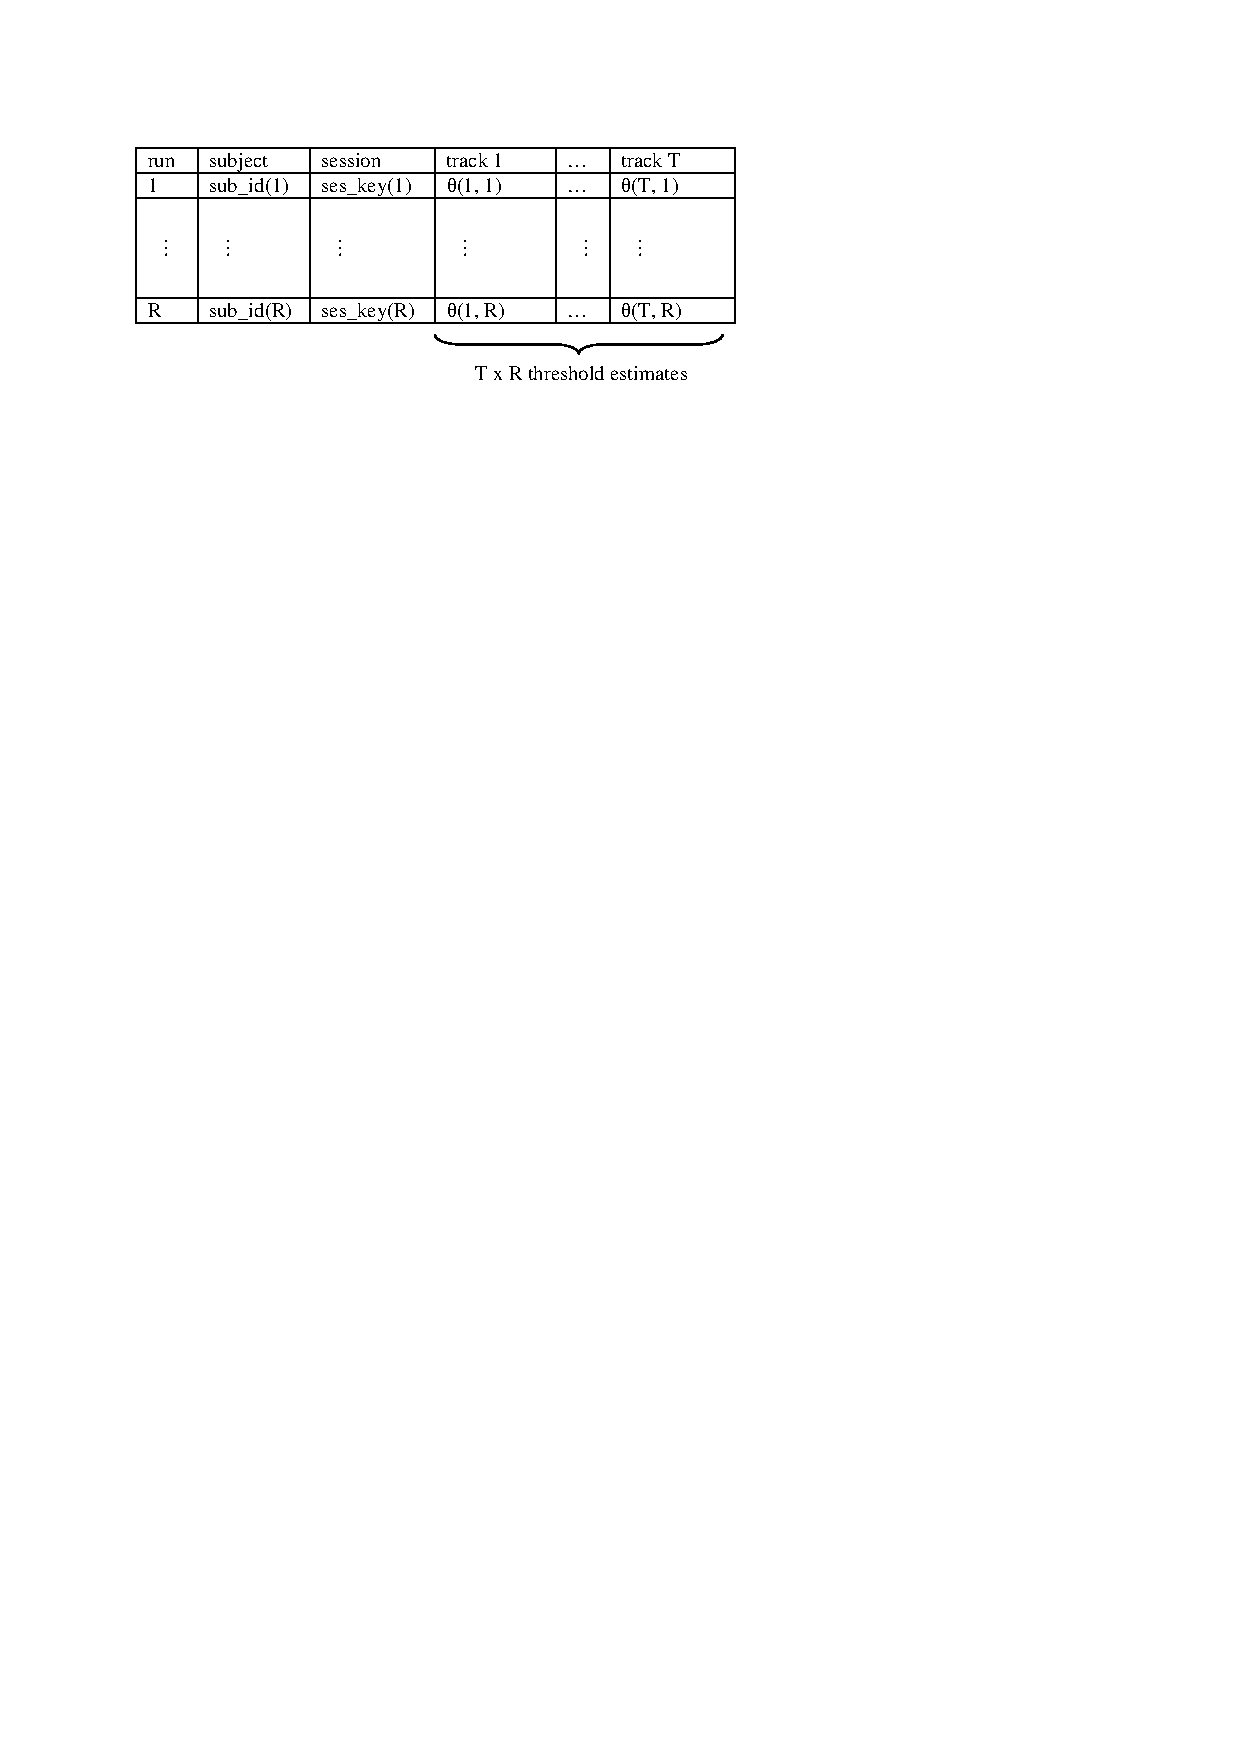
\includegraphics[viewport=2cm 23.2cm 12.5cm 27.4cm, scale=0.75]{exportsheet_ap}}\par
\subfloat[][Repertory grid technique]{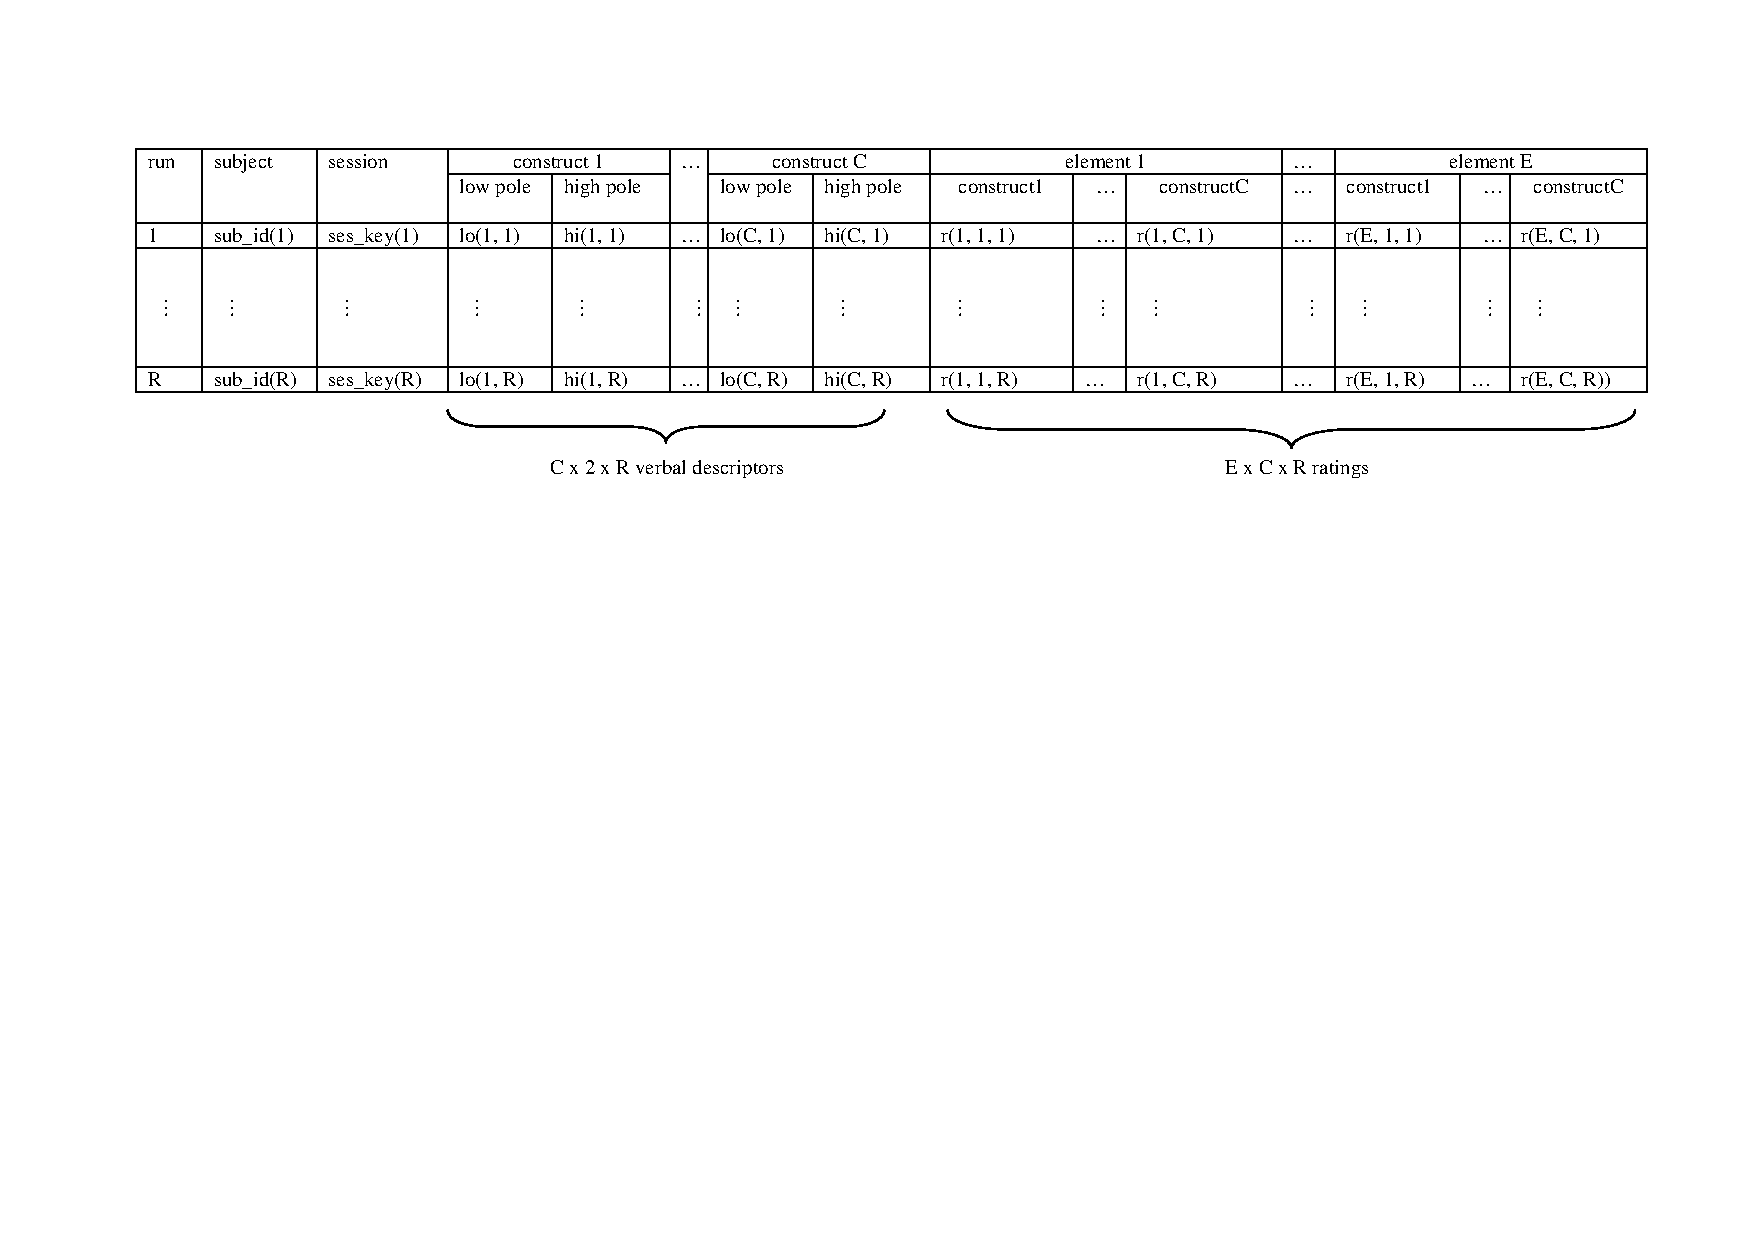
\includegraphics[viewport= 2cm 12.75cm 27.2cm 18.6cm, scale=0.75]{exportsheet_rgt}}\par
\subfloat[][Semantic differential]{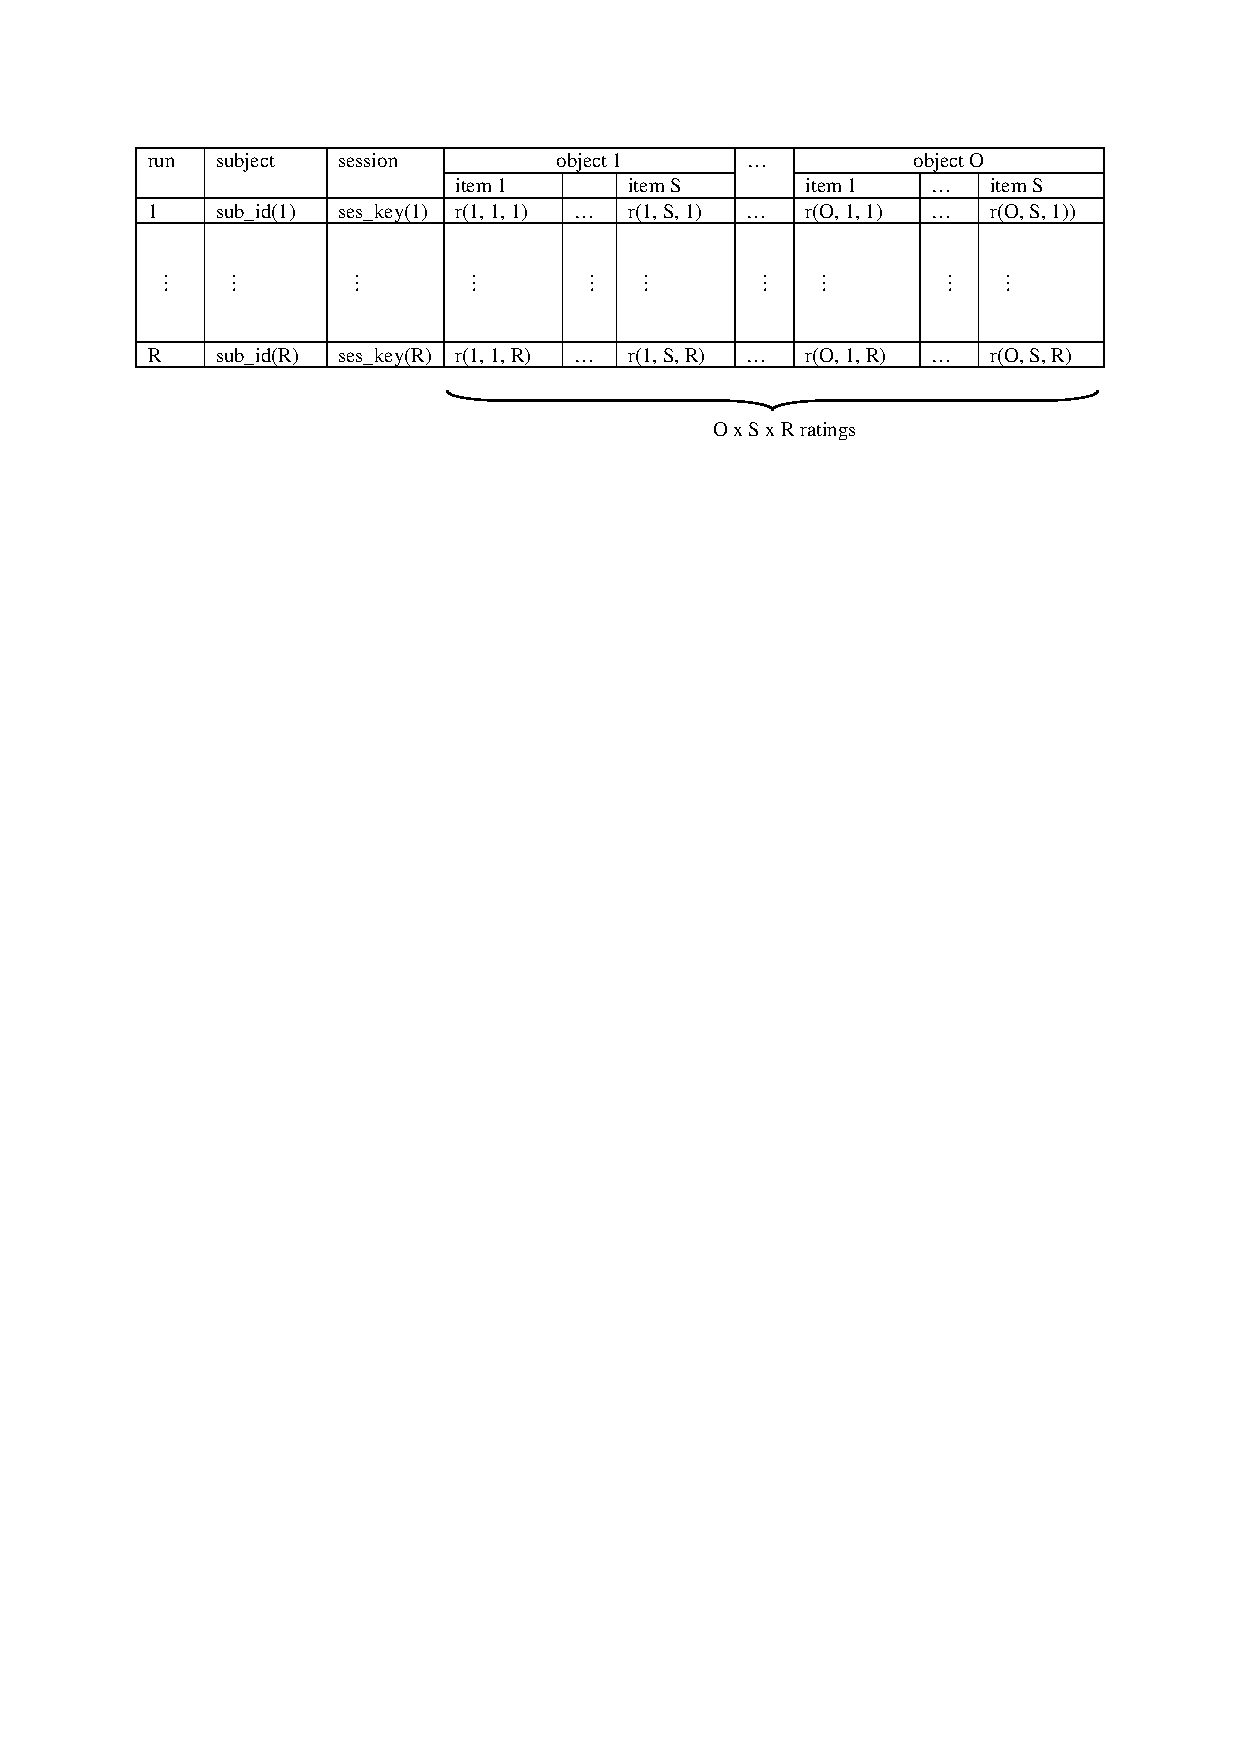
\includegraphics[viewport=2cm 22.2cm 19cm 27.4cm, scale=0.75]{exportsheet_sd}}
\par\smallskip
\caption[Schematic representations of the TSD content.]{Schematic representations of the data export sheets (cp. text on p.~\pageref{export_var}). Note that conceptually the schemes may include missing values, as not every test unit (object, element, triad, track) necessarily has to be assigned to each test run.}
\label{fig:exportsheets}
\end{figure}
\end{landscape}
\clearpage

\begin{landscape}
\begin{figure}[h]\centering
\subfloat[d][ABX]{\includegraphics[]{exportsheet_abx}}\par
\subfloat[e][Spatial Audio Quality Inventory - Level 1]{\includegraphics[]{exportsheet_saqi1}}\par
\subfloat[f][Spatial Audio Quality Inventory - Level 2 'Subject Data']{\includegraphics[]{exportsheet_saqi2}}
\caption[Schematic representations of the TSD content.]
\par\smallskip
\end{figure}
\end{landscape}
\clearpage

\begin{description}
\item [SAQI Empirical Data]
\end{description}
% Tabelle "SAQI Empirical Data"
\begin{longtable}{|c|l|p{10cm}|}
\hline
\multicolumn{1}{|c}{\textbf{Column number}} \vline &  \multicolumn{1}{c}{\textbf{Column name}} \vline &  \multicolumn{1}{c}{\textbf{Encoding}} \vline \endhead
\hline
1&Quality\_ID & 1: difference, 2, 3, 4 etc.... 48: other \\ 
\hline
2&Quality& Quality Name  \\
\hline
3&Category\_ID& 0: 'difference' and 'other' \par  other items have category 1-8  \\
\hline
4&Category&  Category Name  \\
\hline
5&Included& 1: quality was included in test run \par
0: quality was not included in test run\\
\hline
6&Rated&  1: quality was rated (subject heard a difference) \par
0: quality was not rated (subject did not hear a difference) \par
NaN: was not presented in the test  \\
\hline
7&Modification 1&  1: modification 1 was used \par
0: modification 1 was not used   \\
\hline
8&Answer 1&  1: constant \par
2: varying periodically or otherwise rule-based \par
3: varying non regularly \par
NaN: was not presented in the test
  \\
\hline
9&Modification 2&  1: modification 2 was selected by the subject \par
0: modification 2 was not used  \\
\hline
10&Answer 2&  1: steady \par
0: not steady \par
NaN: was not presented in the test  \\
\hline
11&Modification 3&1: modification 3 was used \par
0: modification 3 was not used
   \\
\hline
12&Answer 3.1&  1: 'depending on scene events' was used \par
0: 'depending on scene events' was not used \par
NaN: was not presented in the test
 \\
\hline
13&Answer 3.2&1: 'depending on user interaction' was used \par
0: 'depending on user interaction' was not used \par
NaN: was not presented in the test
    \\
\hline
14&Answer 3.3& 1: 'independent' was used \par
0: 'independent was not used \par
NaN: was not presented in the test
    \\
\hline
15&Rating&  Value of the slider or radio button \par
NaN: was not presented in the test
 \\
\hline
16&Entity1str& 1: assessment entities were included \par
0: assessment entities were not included \par
NaN: was not presented in the test    \\
\hline
17&Entity 1&  User specific name of entity 1 \par
NaN: was not presented in the test \\
\hline
18&Entity1str&  1: Entity 1 was selected \par
0: Entity 1 was not selected \par
NaN: was not presented in the test
  \\
\hline
19&Entity2str&User specific name of entity 2 \par
NaN: was not presented in the test   \\
\hline
20&Entity2str& 1: Entity 2 was selected \par
0: Entity 2 was not selected \par
NaN: was not presented in the test    \\
\hline
21&Entity3str&User specific name of entity 3 \par
NaN: was not presented in the test   \\
\hline
22&Entity3str&  1: Entity 3 was selected \par
0: Entity 3 was not selected \par
NaN: was not presented in the test   \\
\hline
23&Entity4str&User specific name of entity 4  \par
NaN: was not presented in the test  \\
\hline
24&Entity4str& 1: Entity 4 was selected \par
0: Entity 4 was not selected \par
NaN: was not presented in the test    \\
\hline
25&Entity5str&User specific name of entity 5  \par
NaN: was not presented in the test  \\
\hline
26&Entity5str& 1: Entity 5 was selected \par
0: Entity 5 was not selected \par
NaN: was not presented in the test    \\
\hline
27&Entity6str&User specific name of entity 6   \par
NaN: was not presented in the test \\
\hline
28&Entity6str& 1: Entity 6 was selected \par
0: Entity 6 was not selected \par
NaN: was not presented in the test    \\
\hline
29&Entity7str&User specific name of entity 7  \par
NaN: was not presented in the test  \\
\hline
30&Entity7str& 1: Entity 7 was selected \par
0: Entity 7 was not selected \par
NaN: was not presented in the test    \\
\hline
31&Test Condition	& Specifies: Test condition (Stimulus ID \& name) and \par
Reference condition (Stimulus ID \& name), e.g.\par
B1 Test condition (S7 G) vs. A1 Reference condition (S8 H)\\
\hline
32&Scale size& 3, 5 or 7 \\
\hline
33&SAQI version & String, e.g. v.1.3\\
\hline
\caption{Content of the TSD cell 'Subject Data'}
\label{saqi_emp_data}
\end{longtable}
\clearpage

\subsection{The Subfolder \lq log files\rq}\label{logfiles}
This sub folder contains the log files of the runs that have been performed up to the current point. A new log file will always be written right after a test run has been completed. A log file's name consists of the following information in given order: the run number, the subject ID and the session key number. Note that once a log file has been created, it will not be deleted automatically even if the run counter has been reset (cp. sec.~\ref{settingup_testseries}). So if one wants the log files to be deleted, e.g. to achieve a \lqq virginal\rqq\ test series folder, one has to empty this sub folder by hand. Note that if a log file is to be created and one of the same name already exists, the latter will be overwritten.

\subsection{The Subfolder \lq plots\rq}\label{plots}
This sub folder contains all data plots that have been created during the runs so far. At the program's current state plots are only produced for psychophysical adaptive procedures. Each time after a procedure of this type has been performed, a MATLAB\circledR\ figure depicting the respective track will be automatically created. The respective files' names consists of the following information in given order: the run number, the subject ID, the session key number, the section number and the track's number. Additionally or alternatively to the MATLAB\circledR\ figure format one may choose a different file format for the plot being saved in. This can be done by using the menu item \textit{program setup\textbackslash plottings} from the main window's menu bar (see. sec.~\ref{menubar}). Note that once a plot has been created, it will not be deleted automatically even if the run counter has been reset (cp. sec.~\ref{settingup_testseries}). So if one wants the plots to be deleted, e.g. to achieve a \lqq virginal\rqq\ test series folder, one has to empty this subfolder by hand. Note that if a plot is to be created and one of the same name already exists, the latter will be overwritten.


\subsection{The File \lq PS.mat\rq\ (\lqq program settings\rqq)}\label{psmat}
This file is placed in the program folder and contains all settings concerning the program's basic setup. These relate to more technical properties which are (mostly) independent of methodical issues belonging to a certain test series. The standard procedure for adjusting these settings is to use the GUI system (see. chap.~\ref{program_setup}). Though there may be some cases when a different approach yields quicker results. This is for example when one wants to take along these \textit{program settings} to another computer or to switch between several set ups very quickly and there is no time for making all the necessary inputs by hand. In such cases one just might exchange the versions of the file \textit{PS.mat} which is located in the program folder (\lq 2 mfiles\rq). Further adjustments then again can be made by using the GUI system.



%-----------------------------------------
% list of literature
%-----------------------------------------
\clearpage
\bibliographystyle{plainnat}
	\bibliography{literature}

%-----------------------------------------
% list of figures
%-----------------------------------------

\listoffigures

%-----------------------------------------
% appendix
%-----------------------------------------

 


\end{document}
